\documentclass[MSc,french]{ulthese}

  \ifxetex\else \usepackage[utf8]{inputenc} \fi
\usepackage{todonotes}
\usepackage{amsmath,mathtools}
\usepackage{amssymb,amsfonts} 
\usepackage{bm}
\usepackage{fontspec}
\newcommand{\rcursif}{\text{\fontspec{Compagnon Bold}{r}}}
\newcommand{\icursif}{\text{\fontspec{Compagnon Bold}{i}}}
\newcommand{\acursif}{\text{\fontspec{Compagnon Bold}{a}}}
\usepackage{array}
\usepackage{esint}
\usepackage{gensymb}
\usepackage{physics}
\usepackage{extarrows}
\newcommand{\indep}{\perp\!\!\!\perp}
\newcommand{\cov}{\mathrm{cov}}
\newcommand{\dunderline}[1]{\underline{\underline{#1}}}  % Default double underline

\usepackage{algorithm}
\floatname{algorithm}{Algorithme}
\usepackage{algpseudocode}
\algrenewcommand\algorithmicrequire{\textbf{Entrées :}}
\algrenewcommand\algorithmicensure{\textbf{Sorties :}}
\algrenewcommand\algorithmicfor{\textbf{Pour}}
\algrenewcommand\algorithmicwhile{\textbf{Tant que}}
\algrenewcommand\algorithmicif{\textbf{Si}}
\algrenewcommand\algorithmicelse{\textbf{Sinon}}
\algrenewcommand\algorithmicreturn{\textbf{Retourner}}
\algrenewcommand\algorithmicend{\textbf{Fin}}
\algrenewcommand\algorithmicdo{\textbf{faire}}

  \frenchbsetup{%
    StandardItemizeEnv=true,       % format standard des listes
    ThinSpaceInFrenchNumbers=true, % espace fine dans les nombres
    og=«, fg=»                     % caractères « et » sont les guillemets
  }
\usepackage[sc]{caption}
\usepackage{subcaption}
\captionsetup[table]{name=Tableau}
\usepackage{listings}
\usepackage{xcolor}

\definecolor{codegreen}{rgb}{0,0.6,0}
\definecolor{codegray}{rgb}{0.5,0.5,0.5}
\definecolor{codepurple}{rgb}{0.58,0,0.82}
\definecolor{backcolour}{rgb}{0.95,0.95,0.92}
 
\lstdefinestyle{mystyle}{
morekeywords= {arctan2, sin, cos, sqrt, pi, random, uniform, fft, fft2, fftshift, ifft, ifft2, ifftshift, abs, exp, normal, stats, mean, std, j0, i0, arange, tensordot, asnumpy, float32, complex64, __name__, True, False},
    backgroundcolor=\color{backcolour},   
    commentstyle=\color{codegreen},
    keywordstyle=\color{magenta},
    numberstyle=\tiny\color{codegray},
    stringstyle=\color{codepurple},
    basicstyle=\footnotesize,
    breakatwhitespace=false,         
    breaklines=true,                 
    captionpos=b,                    
    keepspaces=true,                 
    numbers=left,                    
    numbersep=5pt,                  
    showspaces=false,                
    showstringspaces=false,
    showtabs=false,                  
    tabsize=2
}
\lstset{style=mystyle}
\renewcommand{\lstlistlistingname}{Extraits de code}
\renewcommand*\lstlistingname{Code}


\setcitestyle{numbers,square}
 \bibliographystyle{plain-fr}


  \titre{Analyse de tavelures laser par apprentissage profond\\Description et planification}

  \auteur{Gabriel Genest}
  \programme{DESS en Intelligence artificielle}
  \direction{Luc Lamontagne}

\begin{document}

\frontmatter                    % pages liminaires

\frontispice                    % production de la page frontispice
\newpage
\tableofcontents 
\newpage
\mainmatter 
\chapter{Description du problème}
Le projet présenté dans ce document est centré sur une problématique touchant l'imagerie et la microscopie. Ces domaines sont au centre de la médecine, de la biophotonique et de plusieurs procédés industriels. Alors que plusieurs cherchent à améliorer la résolution en dépassant le critère de Rayleigh, il existe une modalité d'imagerie simple et naturelle qui a gagné en popularité au cours des dernières années, malgré son émergence au cours des années 1980. Il s'agit de l'imagerie à l'aide des tavelures laser, ou encore \textit{laser speckle imaging} en anglais. Les tavelures laser apparaissent lorsqu'un faisceau de lumière cohérente frappe une surface ayant des aspérités microscopiques de sorte que la lumière est diffusée dans des directions quelconques qu'on simplifie comme aléatoires. Cette diffusion cause différents délais pour les ondes réfléchies, créant des interférences destructives ou constructives lors de la détection de la lumière. La base mathématique des tavelures est bien connue du monde de l'optique statistique (voir les références \cite{goodman_speckle_2020, goodman_statistical_2015, monMemoire} pour plus d'informations), mais une utilisation efficace et rapide des tavelures pour l'imagerie reste une étape cruciale. L’analyse en temps réel des tavelures permet de suivre l’évolution de matériaux ou de phénomènes biologiques. Pour cela, l’apprentissage profond est particulièrement adapté pour automatiser et potentiellement accélérer l'analyse de tavelures, que ce soit dans le domaine spatial ou temporel.
\\ \\
Dans un premier temps, Il existe des méthodes d'analyses statistiques classiques, mais selon la nature stochastique des tavelures, ces méthodes changent et peuvent induire un biais. Ces analyses sont souvent assez lourdes mathématiquement et computationnellement, demandant par exemple plusieurs images dans un film ou encore des propriétés stochastiques bien spécifiques, comme l'ergodicité. Il est possible de modifier ces méthodes si certaines conditions ne sont pas respectées, mais savoir si elles le sont est souvent une autre tâche supplémentaire apportant son lot de défis. Utiliser une approche par apprentissage profond pourrait se spécialiser selon les besoins sans avoir à changer la structure. Si les tavelures sont stationnaires dans l'espace ou non, le réseau devrait être capable de distinguer sans l'intervention humaine lors de l'analyse.
\\ \\
Dans un second temps, plusieurs analyses sont spécifiques à une problématique bien particulière. Cela multiplie les modèles et algorithmes, menant à une recherche difficile pour trouver le bon moyen. Par exemple, si on  est intéressé à calculer la vitesse de déplacement des éléments diffuseurs, on doit avoir un modèle qui la calcule en fonction des données statistiques contenues dans les tavelures. Si on est plutôt intéressé à calculer la rigidité du matériau, on doit utiliser un modèle différent faisant le pont entre les statistiques des tavelures et le module de visco-élasticité, par exemple. Dans ces deux cas, les modèles risquent d'être assez différents ou encore ayant une constructions difficile à implémenter. Utiliser une approche par apprentissage profond pourrait, selon l'entraînement, construire son propre modèle interne et apprendre comment extraire ces informations sans interventions humaines lors de l'analyse.
\\ \\
Comme le phénomène des tavelures laser est autant spatial que temporel, un réseau alliant le contenu spatial et le contenu temporel est considéré. Le réseau aura comme entrée une séquence d'images de tavelures dans le temps et devra sortir l'information pertinente voulue. Dans le cadre de ce projet, cette information est le temps caractéristique de corrélation. La tête du réseau pourrait être modifiée selon l'information à extraire, par exemple la vitesse des diffuseurs. Une architecture mixte composée d'un réseau à convolution (CNN) et d'un réseau récurrent (RNN) sera utilisé, permettant un travail indépendant dans l'espace avec le CNN et l'information du CNN sera par la suite fournie au RNN pour l'aspect temporel. Ainsi, le réseau devrait être capable de cibler les informations pertinentes dans la corrélation spatiale et celle temporelle pour développer son modèle interne.
\newpage
\chapter{Revue de littérature}
\section{Approches classiques}
Plusieurs articles présentent des limitations de modèles qui seront à considérer durant le développement du projet:
\begin{itemize}
\item Briers et al. \cite{briers_laser_2013} expliquent quelques problèmes des modèles fixes de l'analyse des tavelures. Par exemple, certains modèles requiet la connaissance à priori de la distribution de la vitesse des diffuseurs, ce qui est en général pas possible, mais où on peut faire certaines hypothèses. La présence de diffuseurs statiques et dynamiques change aussi l'interprétabilité, car les statistiques changent spatialement, brisant la stationarité et l'ergodicité parfois requise.
\item Liu et al. \cite{liu_choosing_2021} expliquent la multiplication des hypothèses et des modèles. Selon les hypothèses, les modèles changent et deviennent plutôt complexes. Dans cet article, on calcule le le \textit{blood flow index}, soit un indicateur de rapidité de déplacement du sang. Pour y arriver, il faut calculer le contraste et celui-ci est inversement proportionnel au \textit{blood flow index}. Les modèles présentés comportent des paramètres expérimentaux importants, dont le paramètre $\beta$ qu'on rencontre souvent dans la littérature des tavelures et qui est difficile à estimer.
\item Zheng et Mertz \cite{zheng_direct_2022, zheng_correcting_2022} expliquent, dans un premier temps, comment calculer directement le temps de corrélation d'une manière se rapprochant d'une approche sans modèle. On se base sur la théorie des tavelures pleinement développées et on intègre numériquement le contraste. Il y a toutefois les enjeux d'ergodicité: si les tavelures ne sont pas ergodiques, des corrections doivent être apportées, ajoutant une couche d'à priori. De plus, leur algorithme est relativement lourd, utilisant une approche pixel par pixel. Dans un second temps, ils présentent une manière de corriger le biais induit lors du calcul local du contraste spatial. On ajoute encore une couche de complexité et le besoin de savoir si les tavelures sont ergodiques.
\end{itemize}
Ces articles présentent des approches classiques, utilisant des méthodes statistiques.
\section{Apprentissage automatique}
Au cours des dernières années, les chercheurs ont utilisé de plus en plus l'apprentissage machine pour analyser les tavelures:
\begin{itemize}
\item Fredriksson et al. \cite{fredriksson_machine_2019, hultman_speed-resolved_2023} expliquent l'utilisation d'un réseau de neurones artificiels dans le contexte de l'imagerie de tavelures à différents temps d'acquisition. Ils y utilisent un réseau de type perceptron, pleinement connecté avec une seule couche cachée. Le modèle est fourni d'informations extraites d'images de tavelures. Différents réseaux sont initialisés aléatoirement et le meilleur est conservé pour le test. L'utilisation d'une fonction d'activation $\tanh$ est expliquée par le fait que les réseaux l'ayant sont meilleurs que ceux ayant d'autres fonctions d'activation. Ils arrivent à la conclusion que l'apprentissage machine permet aux tavelures laser d'être utilisées et améliorer l'interprétation des images.
\item Kaler et al. \cite{kaler_deep_2023} utilisent différentes approches d'apprentissage automatique pour la détection de graines infectées. Dans un premier temps, ils utilisent des approches plus classiques, comme des SVMs ou des KNNs, mais ensuite combinent des CNNs avec des LSTMs pour une analyse spatio-temporelle. Ils arrivent à la conclusion qu'un modèle à LSTM convolutionnel est meilleur que les autres en général. Cet article est particulièrement intéressant, car il compare plusieurs architecture et une méthode d'analyse robuste, soumettant les architectures à des données originales, sans bruit, puis ajoutant du bruit. De plus, parmis les autres articles, ils sont les seuls à considérer l'aspect spatial et temporel en même temps, profitant des CNNs et des RNNs. Par contre, il s'agit ici d'un problème de classification.
\item Shang et al. \cite{shang_estimation_2025} utilisent un CNN tridimensionnel pour analyser le flot sanguin à partir d'images de tavelures laser. Ils arrivent à des précisions supérieurs à $90\%$, mais font appel à une approche de classification, discrétisant le flot sanguin en plusieurs intervalles. Cet approche peut être avantageuse dans la prédiction, mais on perd de l'information qui est parfois très importante. Il faut aussi bien découper l'espace des résultat pour ne pas avoir un biais trop élevé pour certains intervalles. L'approche de CNN 3D reste toutefois très intéressante.
\end{itemize}
\newpage
\chapter{Choix des modèles}
La programmation des modèles se fera à l'aide du module \textit{PyTorch} du langage de programmation \textit{Python}.
\section{Modèle initial scalaire}
Le modèle principal sélectionné est un mixte entre un réseau convolutionnel et un réseau récurrent, similaire à un modèle présenté dans \cite{kaler_deep_2023}. Ce choix s'explique par la nature des tavelures et des statistiques importantes. Dans un premier temps, l'aspect spatial des tavelures est important à considérer. Comme il s'agit d'un motif d'interférence et d'imagerie, il est possible d'avoir des sections d'images qui sont sans information pertinente. Par exemple, des minimums sombres ou une absence d'illumination laissant des pixels sans intensité. L'avantage du CNN est aussi d'effectuer une sélection des régions importantes, diminuant la dimensionnalité. Il est important de noter que le pooling ne sera pas utilisé entre les couches de CNN, car cette étape diminue la qualité spatiale de l'information, parfois cachée. Il faut aussi mentionner que le réseau CNN ne devra pas être très profond étant donné que seules des statistiques de premier et de second ordre sont pertinente. Utiliser un réseau trop profond pourrait mener à l'extraction d'information non pertinente rendant l'apprentissage plus difficile. À la fin de l'étape de convolution, un mécanisme d'attention spatiale sera utilisé sélectionner les combinaisons de caractéristiques pertinentes. Ce mécanisme est composé d'un petit perception multicouches (MLP) permettant de réduire la dimensionnalité des caractéristiques, forçant le réseau à apprendre comment réduire. Comment les caractéristiques sont spattiales, le MLP sert d'attention spatiale. Cette méthode est inspirée par la structure \textit{Network In Network}\cite{lin_network_2014} et par les architectures \textit{Squeeze-and-Excitation Networks}\cite{hu_squeeze-and-excitation_2017}.
\\ \\
Dans un second temps, un RNN de type GRU sera utilisé pour extraire l'information temporelle à partir de l'attention spatiale. Pour y arriver, un pooling sera appliqué afin de vectoriser les caractéristiques. Par la suite un réseau de type GRU sera entraîné sur une séquence temporelle de tavelures pour extraire l'information scalaire du temps caractéristique. Le choix d'un GRU repose principalement sur sa simplicité contrairement à un LSTM. Il sera toujours possible de tester un LSTM pour vérifier les performances. L'avantage d'un réseau récurrent est dans sa capacité à se souvenir ou oublier l'information passée d'un séquence, ce qui est important dans le cas des tavelures, car pour le temps caractéristique de corrélation, l'information réside dans toute la séquence temporelle et permettra d'estimer un scalaire en prédiction. Le nombre de couches sera petit pour éviter le surapprentissage: débuter avec une seule couche et augmenter au besoin. En plus des caractéristiques extraites du CNN, le temps d'intégration est donné au RNN. Cette quantité est normalement connue lors des expériences et peut servir à déterminer le temps caractéristique.
\section{Modèle secondaire}
Si le temps le permet ou si le modèle principal s'avère problématique, le modèle secondaire est à étudier. Il s'agit d'un réseau récurrent convolutionnel, ConvRNN, de type ConvLSTM, comme utilisé dans \cite{kaler_deep_2023}. Un avantage de cette approche est la possibilité d'extraire une carte locale du temps caractéristique de manière plus naturelle que le modèle précédent. Par contre, l'interprétation du modèle reste un peu plus difficile, demandant plus de paramètres, et pourrait être plus long à l'entraînement. De plus, \textit{PyTorch} ne permet pas explicitement de créer un réseau ayant des couches ConvRRN, que ce soit ConvLSTM ou autre. Il existe toutefois une page GitHub où ConvLSTM est construit sur les bases de \textit{PyTorch}, voir le lien \url{https://github.com/ndrplz/ConvLSTM_pytorch}, ayant plus de 2000 étoiles et 444 \textit{forks}.
\section{Pipeline d'entraînement}
Les données utilisées pour l'entraînement sont présentées au chapitre \ref{donnees}. Les données générées peuvent être sous plusieurs formats, mais on va se contenter à les laisser en \textit{ndarray} de \textit{NumPy}, facilement transférable à \textit{PyTorch}. Si besoin, on peut sauvegrader les données au format \textit{.npy} et les stocker sur un disque. \textit{PyTorch} permet d'utiliser des utilitaires de création de datasets d'entraînement, de validation et de tests, ce qui sera utilisé pour s'assurer d'avoir un entraînement en \textit{batch} avec un certain aléatoire pour diversifier le contenu de chaque \textit{batch}.
\begin{figure}[h!!]
    \centering
    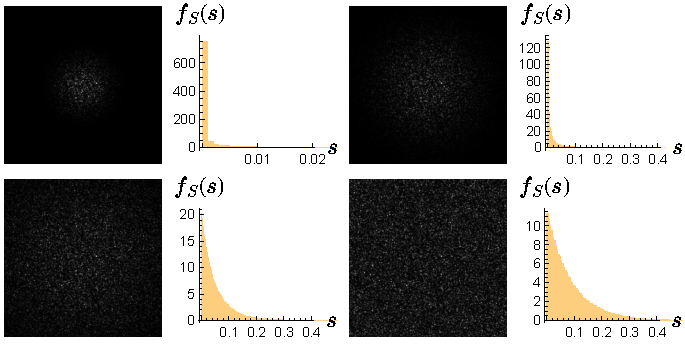
\includegraphics[width=1\linewidth]{images/staticWithGaussMask.pdf}
    \caption{Simulations de tavelures pleinement développées où un masque gaussien est appliqué sur l'intensité résultante, montrant l'effet d'un faisceau gaussien sur la tache laser. On montre que plus la tache laser est petite sur l'image, plus l'intensité est biaisée vers $0$. De telles images doivent être normalisée judicieusement. Image tirée de \cite{monMemoire}.}
    \label{fig:specklesGaussianMask}
\end{figure}
\\
Le modèle initial est schématiquement présenté à la figure \ref{fig:schema_v1}, avec les hyperparamètres initiaux. Ceux-ci peuvent changer durant le développement du projet. Pour l'entraînement, plusieurs modalités de simulations seront présentées aléatoirement à chaque batch. Les modalités pour chaque séquence seront décrites dans un fichier csv de métadonnées. Par modalité, on fait référence au paramètres physiques de l'imagerie, comme le temps caractéristique, le temps d'intégration et la fonction de corrélation. Comme ces paramètres jouent un rôle important dans l'entraînement, plusieurs instances de chaque combinaisons seront requises. Le DataLoader permet de bien distribuer aléatoirement les diverses simulations pour que le réseau aie une vue d'ensemble et non seulement quelques exemples ayant les même propriétés.
\begin{figure}[h!!]
    \centering
    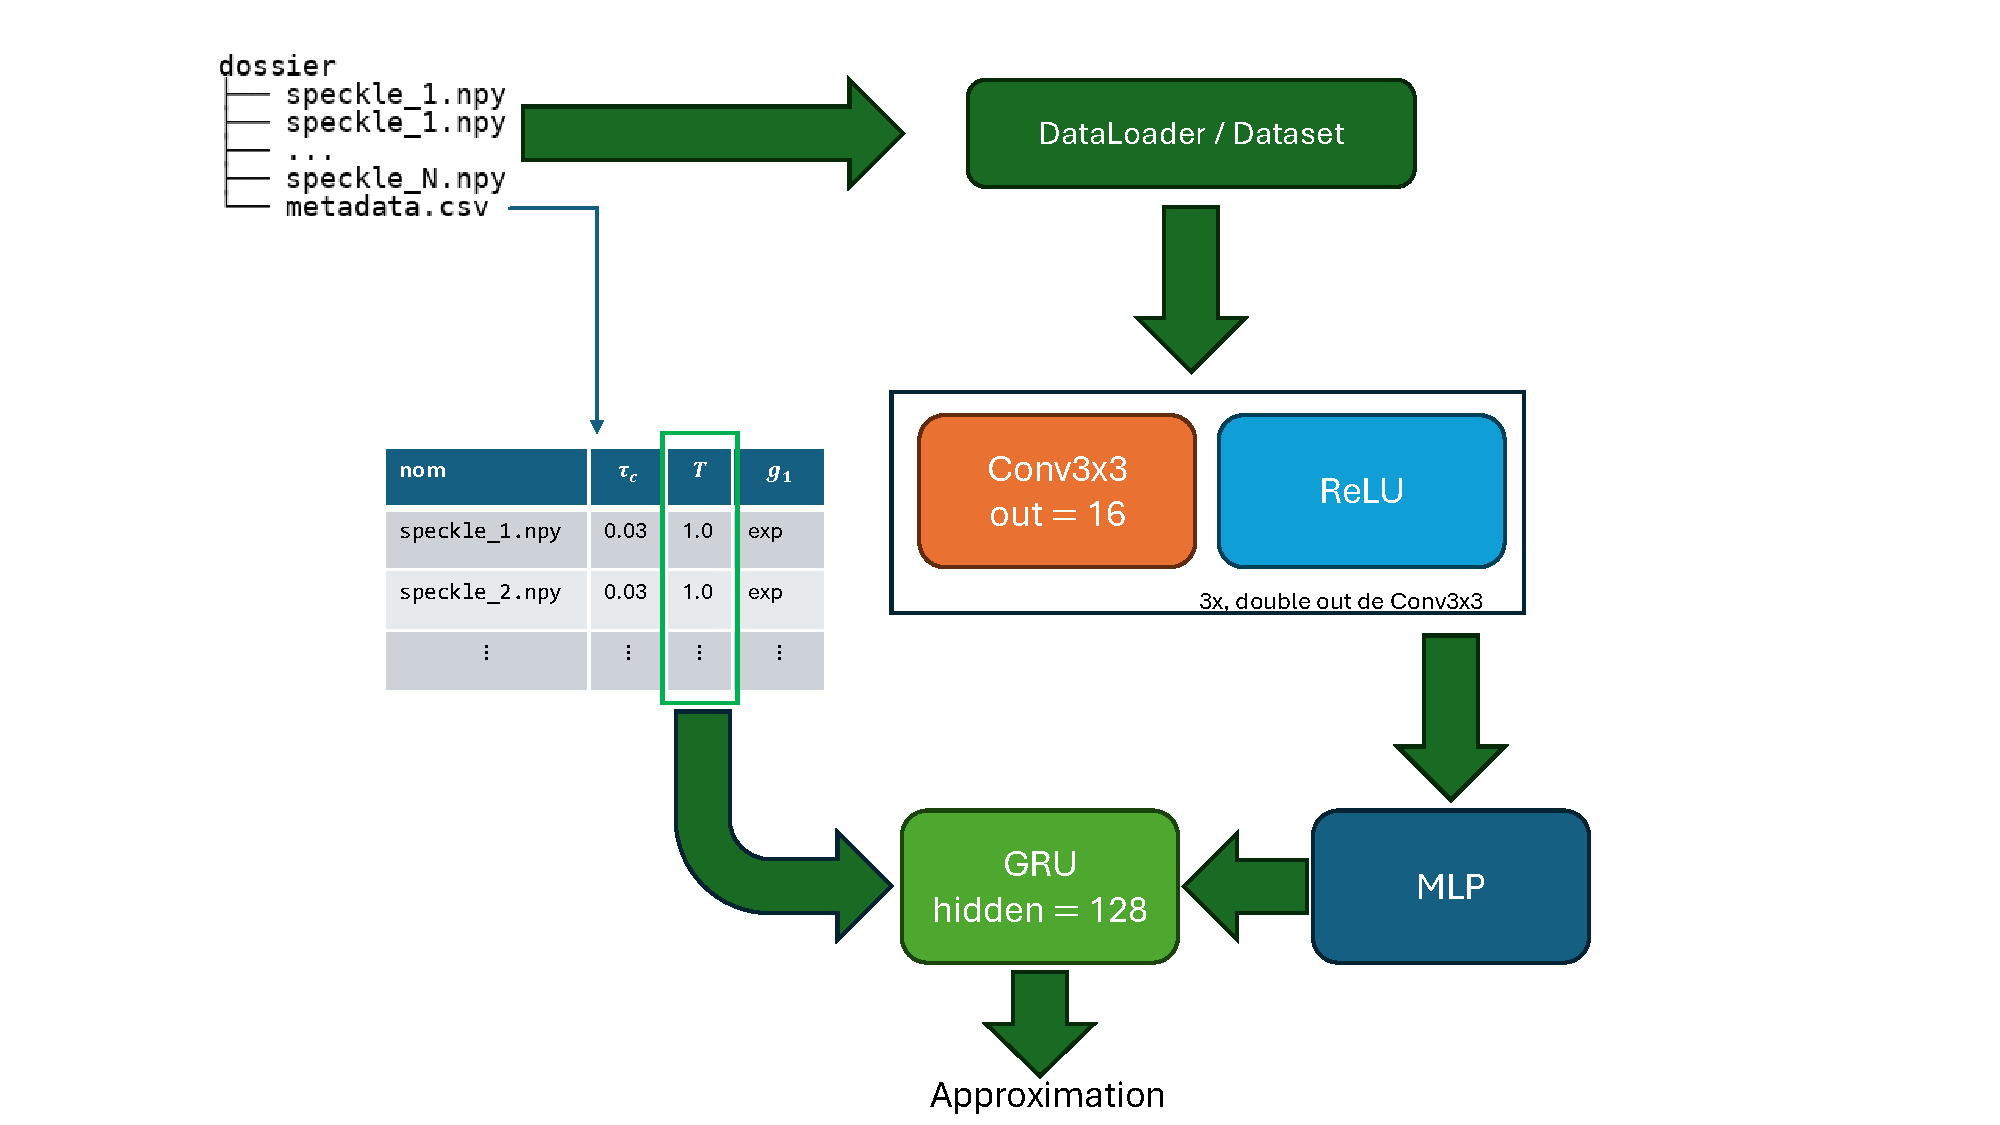
\includegraphics[width=1\linewidth]{images/modele_DESS_projet_v2.pdf}
    \caption{Schéma montrant le pipeline du réseau utilisé pour le projet. Les hyperparamètres peuvent changer au cours du développement.}
    \label{fig:schema_v1}
\end{figure}
\newpage
\chapter{Données du modèle}\label{donnees}
\section{Générations de base}
Les données d'entraînement du modèle seront générées numériquement selon un algorithme précis. De cette manière, on peut modifier les paramètres statistiques des tavelures comme on veut. De plus, une grande quantité de données peuvent être générées dans une fraction du temps que demande un montage expérimental. L'algorithme est basé principalement sur \cite{james_simulation_2021} où on présente une façon de simuler l'intégration temporelle des tavelures. Toutefois, cet algorithme ne simule pas de séries temporelles. Initialement, on génère les phaseurs selon l'Algorithme \ref{alg:specklesTempInt}.
\begin{algorithm}
    \caption{Simulation de tavelures pleinement développées intégrées temporellement}\label{alg:specklesTempInt}
\begin{algorithmic}
\Require $N\in\mathbb{N}^*$, $R\in\mathbb{R}^{*}_+$, $N_T\in\mathbb{N}^*$, $\Delta T \in \mathbb{R}^*_+$, $g:\mathbb{R}\to\mathbb{R}$
\Ensure $I$ avec $I \in {\mathbb{R}}^{N\times N}_+$
\State Générer $\Theta \in [-\pi,\pi]^{N \times N}$ avec $\Theta_{ik} \sim \mathcal{U}(-\pi,\pi)$ indépendants
\State Définir $\Sigma \in \{0, 1\}^{N\times N}$ comme un disque centré de rayon $R$
\State $T \gets [0, \Delta T, 2\Delta T, \dots, (N_T - 1)\Delta T]$
\State $I \gets \textbf{0}_{N\times N}$
\State $G\gets \textbf{0}_{N_T\times N_T}$
\For{$i = 1$ \textbf{à} $N_T$}
    \For{$k = 1$ \textbf{à} $N_T$}
        \State $G_{ik} \gets g(|T_i - T_j|)$
    \EndFor
\EndFor
\State $\lambda \gets \text{eigvals}(G)/N_T$ \Comment{$\text{eigvals}$ calcule les valeurs propres}
\For{$n = 1$ \textbf{à} $N_T$}
	\State $A \gets \exp{j\Theta}$ \Comment{Exponentielle terme à terme}
	\State $A \gets \mathcal{F}_{2D}(A)\sqrt{\lambda_n}$\Comment{Transformée de Fourier 2D}
	\State $A \gets \Sigma\odot A$
	\State $A \gets \mathcal{F}_{2D}^{-1}(A)$\Comment{Transformée de Fourier inverse 2D}
	\State $A_{\mathbb{R}} \gets \abs{A}$ \Comment{Module terme à terme}
	\State $I \gets I + A_{\mathbb{R}}^2$ \Comment{Carré terme à terme}
\EndFor
\end{algorithmic}
\end{algorithm}
\newpage
Pour une série temporelle, sans intégration temporelle, on doit modifier la création des amplitudes complexes pour ajouter une dimension temporelle ayant une certaine corrélation, comme montré à l'Algorithme \ref{alg:specklesBaseTS}.
\begin{algorithm}
    \caption{Simulation temporelle de tavelures pleinement développées}\label{alg:specklesBaseTS}
\begin{algorithmic}
\Require $N\in\mathbb{N}^*$, $R\in\mathbb{R}_{+}^*$, $P\in\mathbb{N}^*$, $C\in\mathbb{R}^{P\times P}$
\Ensure $(A_\mathbb{R}, I)$ avec $A_\mathbb{R} \in \mathbb{R}^{P\times N\times N}$ et $I \in \mathbb{R}_+^{P \times N\times N}$
\State Générer $\mathcal{R} \in \mathbb{R}^{P \times N \times N}$ avec $\mathcal{R}_{pik} \sim \mathcal{N}\left(0, \frac{1}{2}\right)$ et $\rho\left(\mathcal{R}_{pik}, \mathcal{R}_{p'i'k'}\right) = \begin{cases}
    C_{pp'} & \text{si }(i, k) = (i', k')\\
    0 & \text{sinon}
\end{cases}$
\State Générer $\mathcal{I} \in \mathbb{R}^{P\times N\times N}$ avec $\mathcal{I}_{pik} \sim \mathcal{N}\left(0, \frac{1}{2}\right)$ et $\rho\left(\mathcal{I}_{pik}, \mathcal{I}_{p'i'k'}\right) = \begin{cases}
    C_{pp'} & \text{si }(i, k) = (i', k')\\
    0 & \text{sinon}
\end{cases}$
\State Définir $\Sigma \in \{0, 1\}^{N\times N}$ comme un disque centré de rayon $R$
\State $A\gets \textbf{0}_{P\times N \times N}$
\For{$p = 1$ \textbf{à} $P$}
    \State $A_p \gets \mathcal{R}_p + j\mathcal{I}_p$
    \State $A_p \gets \mathcal{F}_{2D}(A_p)$
    \State $A_p \gets \Sigma \odot A_p$
    \State $A_p \gets \mathcal{F}_{2D}^{-1}(A_p)$
\EndFor
\State $A_{\mathbb{R}} \gets \abs{A}$
\State $I \gets A_{\mathbb{R}}^2$
\end{algorithmic}
\end{algorithm}
La corrélation provenant de la matrice de corrélation $C$ est conservée dans le champ réel $A_\mathbb{R}$ et la corrélation de l'intensité $I$ en est simplement le carré. 
\section{Générations avancées: à utiliser}
Il est possible de mettre en commun l'Algorithme \ref{alg:specklesTempInt} et l'Algorithme \ref{alg:specklesBaseTS}: on génère les amplitudes selon l'Algorithme \ref{alg:specklesBaseTS}, permettant ainsi une corrélation temporelle spécifique, puis ensuite on se base sur l'Algorithme \ref{alg:specklesTempInt}. On obtient l'Algorithme \ref{alg:specklesTS_TempInt}. Un avantage de cet algorithme est qu'il génère des séries temporelles stationnaires grâce à la création des séries temporelles multinormales, contrairement à d'autres algorithmes trouvés dans la littérature. On peut alors décider de la corrélation temporelle, tant qu'elle donne une matrice de corrélation valide, c'est-à-dire positive (semi) définie. On peut aussi moduler le temps d'intégration simulée, donnant des images plus ou moins floues. Un désavantage de cette approche est sa complexité en mémoire. En effet, on doit générer $N_T \times P \times N \times N$ amplitudes complexes, même si au final on perd la première dimension à l'aide d'une réduction. L'interdépendance des $P$ champs $N\times N$ fait aussi en sorte qu'on ne peut pas les générer \textit{on the go}, on doit les créer toutes en même temps pour que la dépendance temporelle soit cohérente. Il est toutefois possible de vectoriser l'algorithme pour tirer avantage des architectures GPU. La première étape de vectorisation se trouve dans la boucle interne finale sur $P$, ainsi les opérations internes peuvent se faire en bloc. Une deuxième étape est d'aussi vectoriser la boucle externe finale sur $N_T$, mais on multiplie la mémoire requise en une passe. Soit on a beaucoup de VRAM à consacrer, soit on doit avoir de petites simulations. En se limitant par contre à la boucle interne, des GPUs de moyenne gamme peuvent très bien gérer des simulations intéressantes. On peut aussi s'assurer de libérer l'espace dès que possible ou encore de restreindre la précision des flottants, par exemple à $32$ bits. De cette manière, les amplitudes complexes sont sur $64$ bits, ce qui est suffisant en général.
\begin{algorithm}
    \caption{Simulation temporelle de tavelures pleinement développées intégrées temporellement}\label{alg:specklesTS_TempInt}
\begin{algorithmic}
\Require $N\in\mathbb{N}^*$, $R\in\mathbb{R}_{+}^*$, $N_T\in\mathbb{N}^*$, $\Delta T\in\mathbb{R}^*_+$, $g: \mathbb{R}\to\mathbb{R}$, $P\in\mathbb{N}^*$
\Ensure $I$ avec $I \in \mathbb{R}_+^{P \times N\times N}$
\State Définir $\Sigma\in\{0,1\}^{N\times N}$ comme un disque centré de rayon $R$
\State $T \gets [0, \Delta T, 2\Delta T, \dots, (N_T - 1)\Delta T]$
\State $I\gets \textbf{0}_{P\times N \times N}$
\State $G\gets \textbf{0}_{N_T \times N_T}$
\State $c \gets \textbf{0}_{P}$
\For{$p = 0$ \textbf{à} $P-1$}
	\State $c_p\gets g(p\cdot (N_T-1)\Delta T)$
\EndFor
\State $C \gets \text{Toeplitz}(c)$ \Comment{Construit une matrice Toeplitz avec première ligne $c$}
\For{$i = 1$ \textbf{à} $N_T$}
	\For{$k = 1$ \textbf{à} $N_T$}
		\State $G_{ik} \gets g(\abs{T_i - T_j})$
	\EndFor
\EndFor
\State $\lambda \gets \text{eigvals}(G) / N_T$
\For{$n = 1$ \textbf{à} $N_T$}
	\State Générer $\mathcal{R} \in \mathbb{R}^{P \times N \times N}$, $\mathcal{R}_{pik} \sim \mathcal{N}\left(0, \frac{1}{2}\right)$ et $\rho\left(\mathcal{R}_{pik}, \mathcal{R}_{p'i'k'}\right) = \begin{cases}
    C_{pp'} & \text{si }(i, k) = (i', k')\\
    0 & \text{sinon}
\end{cases}$
\State Générer $\mathcal{I} \in \mathbb{R}^{P\times N\times N}$, $\mathcal{I}_{pik} \sim \mathcal{N}\left(0, \frac{1}{2}\right)$ et $\rho\left(\mathcal{I}_{pik}, \mathcal{I}_{p'i'k'}\right) = \begin{cases}
    C_{pp'} & \text{si }(i, k) = (i', k')\\
    0 & \text{sinon}
\end{cases}$
	\For{$p = 1$ \textbf{à} $P$}
		\State $A_p \gets \mathcal{R}_p + j\mathcal{I}_p$
		\State $A_p \gets \mathcal{F}_{2D}(A_p)\sqrt{\lambda_n}$
		\State $A_p\gets \Sigma \odot A_p$
		\State $A_p \gets \mathcal{F}^{-1}_{2D}(A_p)$
		\State $A_\mathbb{R} \gets \abs{A_p}$
		\State $I_p \gets I_p + A_\mathbb{R}^2$
	\EndFor
\EndFor
\end{algorithmic}
\end{algorithm}
\newpage
La génération des données se fera à l'aide du langage de programmation \textit{Python}, en utilisant les puissantes librairies \textit{NumPy} et \textit{SciPy} principalement. De plus, pour l'accélération GPU, la librairie \textit{CuPy} sera aussi importante, étant essentiellement un portage de \textit{NumPy} (et d'un peu de \textit{SciPy}) sur les cartes graphiques compatibles CUDA\footnote{Aussi disponible pour les architectures ROCm, mais à l'état expérimental.}. Pour plus d'information sur le module, visiter le site web \url{https://cupy.dev/}.
\\ \\
Si le temps le permet, il serait aussi intéressant de tester différentes variantes, notamment l'ajout de bruit, la non uniformité de la tache laser et la variation spatiale du temps caractéristique de corrélation. Les deux premiers cas sont relativement triviaux, tandis que le dernier requiert une refonte de l'algorithme à l'étape de création des amplitudes complexes et lors de la pondération par les valeurs propres. Pour l'instant, seules les tache uniforme sans bruit et de temps de corrélation stationnaire dans l'espace sont considérés. La figure \ref{fig:expSimEx} montre trois simulations d'une même séquence où le temps d'intégration est de $0.03$ seconde et le temps caractéristique est de $1$ seconde. La corrélation de la séquence au complet est présentée à la figure \ref{fig:corrExp}. À la figure \ref{fig:gaussSimEx}, on montre trois simulations aussi d'une même séquence, avec les même paramèrtres, sauf la corrélation qui est maintenant gaussienne au lieu d'exponentielle. La corrélation de la séquence au complet est présentée à la figure \ref{fig:corrGauss}. Ce genre d'images seront générées pour différents paramètres et serviront à l'entraînement, la validation et le test.
\begin{figure}[h!!]
    \centering
    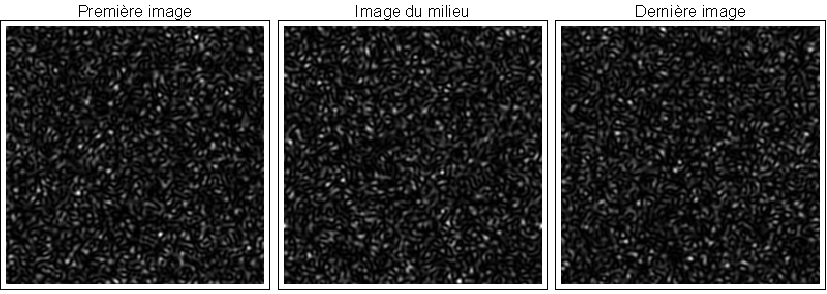
\includegraphics[width=1\linewidth]{images/images_exp.pdf}
    \caption{Exemple d'une modalité de simulation de tavelures. Ici, la corrélation temporelle est exponentielle.}
    \label{fig:expSimEx}
\end{figure}
\begin{figure}[h!!]
    \centering
    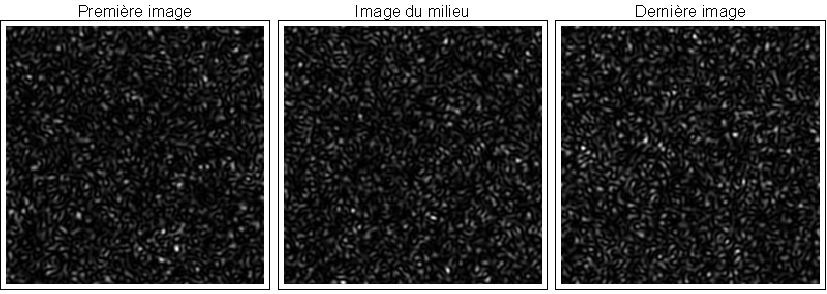
\includegraphics[width=1\linewidth]{images/images_gauss.pdf}
    \caption{Exemple d'une modalité de simulation de tavelures. Ici, la corrélation temporelle est gaussienne.}
    \label{fig:gaussSimEx}
\end{figure}
\begin{figure}
     \centering
     \begin{subfigure}[b]{0.49\textwidth}
         \centering
         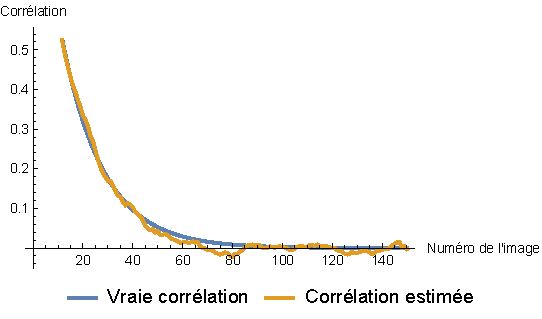
\includegraphics[width=\textwidth]{images/corr_exp.pdf}
         \caption{Corrélation temporelle théorique et estimée d'une séquence temporelle de $150$ simulations de tavelures pour une corrélation exponentielle.}
         \label{fig:corrExp}
     \end{subfigure}
     \hfill
     \begin{subfigure}[b]{0.49\textwidth}
         \centering
         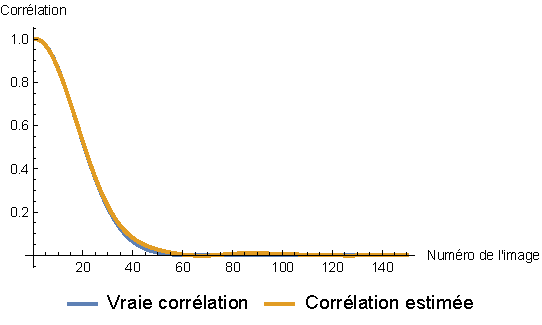
\includegraphics[width=\textwidth]{images/corr_gauss.pdf}
         \caption{Corrélation temporelle théorique et estimée d'une séquence temporelle de $150$ simulations de tavelures pour une corrélation gaussienne.}
         \label{fig:corrGauss}
     \end{subfigure}
\end{figure}
\newpage
\chapter{Évaluation du modèle}
Pour évaluer le modèle, quelques points sont à étudier. Premièrement, on va évaluer les performances pour des images dites \textit{idéales}, donc une tache laser infinie. Comme le réseau donne le temps caractéristique de corrélation, une métrique de log erreur absolue sera utilisé, soit:
\begin{align*}
LEA = \abs{\log{\hat{\tau}_c} - \log{\tau_c}}.
\end{align*}
Pour une même combinaison de paramètres de simulations, mais pour différentes réalisations, on va aussi effectuer un test $t$ de Student (ou une variante selon la distribution des écarts) pour vérifier si le biais du modèle est statistiquement nul, à un seuil de $5\%$. Une troisième métrique est le score $R^2$ entre les estimations et les vraies valeurs pour différents temps caractéristiques. Essentiellement, étape par étape, on a:
\begin{enumerate}
\item Entraînement du modèle;
\item Évaluation du modèle:
\begin{enumerate}
\item Itérer sur un ensemble de validation avec des paramètres identiques et différents,
\item Calculer la $LEA$ pour tous les éléments,
\item Calculer le score $R^2$ sur $LEA$ pour tous les éléments;
\item Faire des tests $t$ pour tous les éléments ayant les mêmes propriétés.
\end{enumerate}
\end{enumerate}
De cette manière, on obtient de l'information sur la justesse générale du modèle avec le $LER$, mais aussi de l'information sur la variance expliquée avec le score $R^2$ et sur le biais statistique du modèle avec les tests $t$.
\newpage
\chapter{Tâches à accomplir}
\section{Génération des données}
La première tâche à accomplir consiste à générer plusieurs jeux de données ayant des paramètres de simulation différents, mais aussi identiques. Étant donné la nature statistique et probabiliste des simulations, différentes réalisations ayant les même paramèrtres donnent des séquences différentes. Ainsi, en donnant plusieurs séquences de paramètres identiques, le réseau n'apprend pas que pour une seul séquence, mais apprend une généralisation.
\\ \\
Le code pour générer les données selon l'Algorithme \ref{alg:specklesTS_TempInt} existe déjà, bien que sous une forme qui pourrait être plus élégante, comme utiliser le paradigme orienté objet. Quelques heures seraient mises pour finaliser et tester un code complet. Le code devrait permettre d'itérer sur plusieurs paramèrtres, faire quelques simulations par combinaison et enregistrer les données sur disque. L'approche de génération par GPU sera préconisée, car elle accélère grandement l'exécution du code.
\section{Développement du pipeline d'entraînement: DataLoader et Dataset}
Pour bien tirer profit de \textit{PyTorch}, il sera important d'implémenter des classes permettant de charger les données de manière aléatoire parmis les combinaisons de paramètres et de former des lots pour l'entraînement. La documentation web explique bien comment procéder, donc quelques heures seront requises pour s'assurer d'avoir un pipeline d'accès aux données qui est efficace et pratique. Il sera important de ne pas charger toutes les données d'entraînement en même temps, cela risque de surcharger la RAM. Seulement celles requises pour le lot courant seront chargées, avec peut-être quelques lots en buffer. Implémenter une approche parallèle pourrait être pertinente, soit charger les données en même temps qu'un lot est utilisé. À voir à quel point cela est faisable et raisonnable.
\section{Développement du pipeline d'entraînement: Modèle}
Le premier modèle présenté plus tôt dans ce document sera implémenté à l'aide de \textit{PyTorch}. L'implémentation initiale ne devrait pas être trop longue. Ce qui risque de demander plus de temps est l'optimisation des hyperparamètres. Toutefois, lorsque l'architecture de base sera présente, modifier les hyperparamètre revient majoritairement à remplacer quelques bouts de code. Selon le temps requis pour l'entraînement d'un modèle, des comparaisons pourraient être effectuées durant la nuit. En plus d'un ordinateur portable, un ordinateur de bureau est disponible. Lors des heures de cours, celui-ci n'est pas utilisé et pourra servir de machine principale pour l'entraînement. Si possible, contrôler cette machine à distance sera considéré. L'évaluation étant automatique, plusieurs entraînements peuvent être itérés sans interaction humaine.
\section{Décision du modèle}
Après optimisation des hyperparamètres, il sera décidé de quelle configuration choisir. Si les résultats ne sont pas intéressant et que plusieurs combinaisons d'hyperparamètres ont été explorées, le deuxième modèle sera considéré. Le principal problème avec le second modèle est qu'il n'est pas faisable facilement avec \textit{PyTorch}, on doit construire la mécanique interne. La présence d'un répertoire GitHub est intéressante, mais la qualité de l'implémentation peut être problématique.
\section{Exploration complémentaire (si le temps le permet)}
Dans le cas où le projet avance très bien et qu'il reste suffisamment de temps, le modèle pourrait être modifié pour changer la sortie du réseau. Pour l'instant, une sortie scalaire est considérée, mais une carte locale de temps de corrélation serait plus précise pour des processus dynamiques qui ne sont pas stationnaire dans l'espace, comme différents tissus biologiques ayant différentes rigidités.
\newpage
\chapter{Expérimentations initiales}
L'expérimentation initiale s'est principalement faite en deux étapes. Dans un premier temps, plusieurs séquences de paramètres statistiques et physiques différents sont fournies au modèle. Or, ce ne s'est pas avéré efficace pour tester la capacité d'apprentissage du modèle: les performances étaient très mauvaises et le réseau ne convergeait pas vers une solution à faible perte. On peut expliquer les problèmes par la haute dimensionnalité de l'espace des paramètres physiques et statistiques. En effet, on fait varier le temps caractéristique $\tau_c$ sur une plage dynamique importante, de même que pour le temps d'intégration $T$. On a alors un sous ensemble non négligeable de $\mathbb{R}^2$ où le réseau doit apprendre l'interdépendance des images et des paramètres. De plus, on fait aussi varier la fonction de corrélation temporelle entre une exponentielle et une gaussienne. Le problème devient rapidement lourd, surtout en mémoire. On ne peut pas efficacement apprendre seulement sur de petits sous-ensembles de l'espace des paramètres.\\ \\
\section{Sur-apprentissage}
Pour la deuxième étape, il a été nécessaire de retourner à la base. Il est important en apprentissage automatique de déterminer si réellement un réseau peut apprendre. On doit donc s'assurer que le réseau puisse sur-apprendre un petit jeu de données. Pour y arriver, le modèle initial est modifié pour considérer le temps d'intégration comme une caractéristique fournie au réseau récurrent. De plus, une restriction sur le domaine des paramètres de simulation est requise. On fait seulement varier le temps caractéristique pour un temps d'intégration spécifique, ici fixé à $1$ (les unités sont arbitraires). Le temps caractéristique est divisé en trois modalités: plus petit que $T$, même ordre que $T$ et plus grand que $T$. On divise aussi l'entraînement selon la fonction de corrélation. Ces deux séparations permettent de déterminer si une modalité de temps caractéristique ou une fonction de corrélation cause un entraînement problématique. Voici la démarche de sur-apprentissage d'un petit jeu de données:
\begin{itemize}
\item Pour $\tau_c < T$:
	\begin{enumerate}
	\item Générer $8$ $\tau_c$ dans un espace linéaire de $10^{-2}$ à $0.5$;
	\item Simuler avec répétition de $2$ pour chaque $\tau_c$ avec corrélation exponentielle;
	\item Entraîner sur $300$ époques;
	\item Simuler avec répétition de $2$ pour chaque $\tau_c$ avec corrélation gaussienne;
	\item Entraîner sur $300$ époques;
	\end{enumerate}
\item Pour $\tau_c\approx T$:
	\begin{enumerate}
	\item Générer $8$ $\tau_c$ dans un espace linéaire de $0.8$ à $1.2$;
	\item Simuler avec répétition de $2$ pour chaque $\tau_c$ avec corrélation exponentielle;
	\item Entraîner sur $300$ époques;
	\item Simuler avec répétition de $2$ pour chaque $\tau_c$ avec corrélation gaussienne;
	\item Entraîner sur $300$ époques;
	\end{enumerate}
\item Pour $\tau_c > T$:
	\begin{enumerate}
	\item Générer $8$ $\tau_c$ dans un espace linéaire de $1.5$ à $20$;
	\item Simuler avec répétition de $2$ pour chaque $\tau_c$ avec corrélation exponentielle;
	\item Entraîner sur $300$ époques;
	\item Simuler avec répétition de $2$ pour chaque $\tau_c$ avec corrélation gaussienne;
	\item Entraîner sur $300$ époques;
	\end{enumerate}
\end{itemize}
Il est aussi important d'avoir une optimisation adéquate lors de l'entraînement. Le test de sur-apprentissage s'est effectué à l'aide de l'optimiseur Adam\cite{kingma_adam_2014} avec deux taux d'apprentissage. On a utilisé un taux de $10^{-3}$, puis un taux de $10^{-4}$. La perte est la perte $L1$, mais appliquée sur le logarithme de la sortie et de la cible, donc la log erreur absolue. Comme les temps caractéristique sont généralement petits, utiliser le logarithme permet d'avoir une échelle intéressante limitant la perte du gradient. La figure \ref{fig:allLossesOverfitPlusPetit} montre les pertes en entraînement pour le régime $\tau_c < T$, et ce pour les deux fonctions de corrélations et les deux taux d'apprentissage. Dix entraînement pour un même ensemble de paramètres physiques ont été faits, permettant de confirmer l'entraînement et non simplement de la chance pour un essai unique. On remarque que les deux corrélations donnent un comportement similaire d'entraînement, ce qui laisse croire qu'il n'y a pas de difficulté spécifique à l'une ou l'autre. On remarque aussi qu'un taux d'apprentissage plus élevé, soit $10^{-3}$ donne un entraînement plus rapide, convergeant vers de plus petites pertes avant le taux de $10^{-4}$. La figure \ref{fig:moyennesLossesOverfitPlusPetit} montre la moyenne des quatre cas étudiés à la figure \ref{fig:allLossesOverfitPlusPetit}, permettant de mieux visualiser la meilleure performance du taux $10^{-3}$, mais aussi le comportement similaire des deux fonctions de corrélation, bien que le cas gaussien semble devenir plus difficile à apprendre à partir de l'époque $200$.
\newpage
\begin{figure}[h!!]
    \centering
    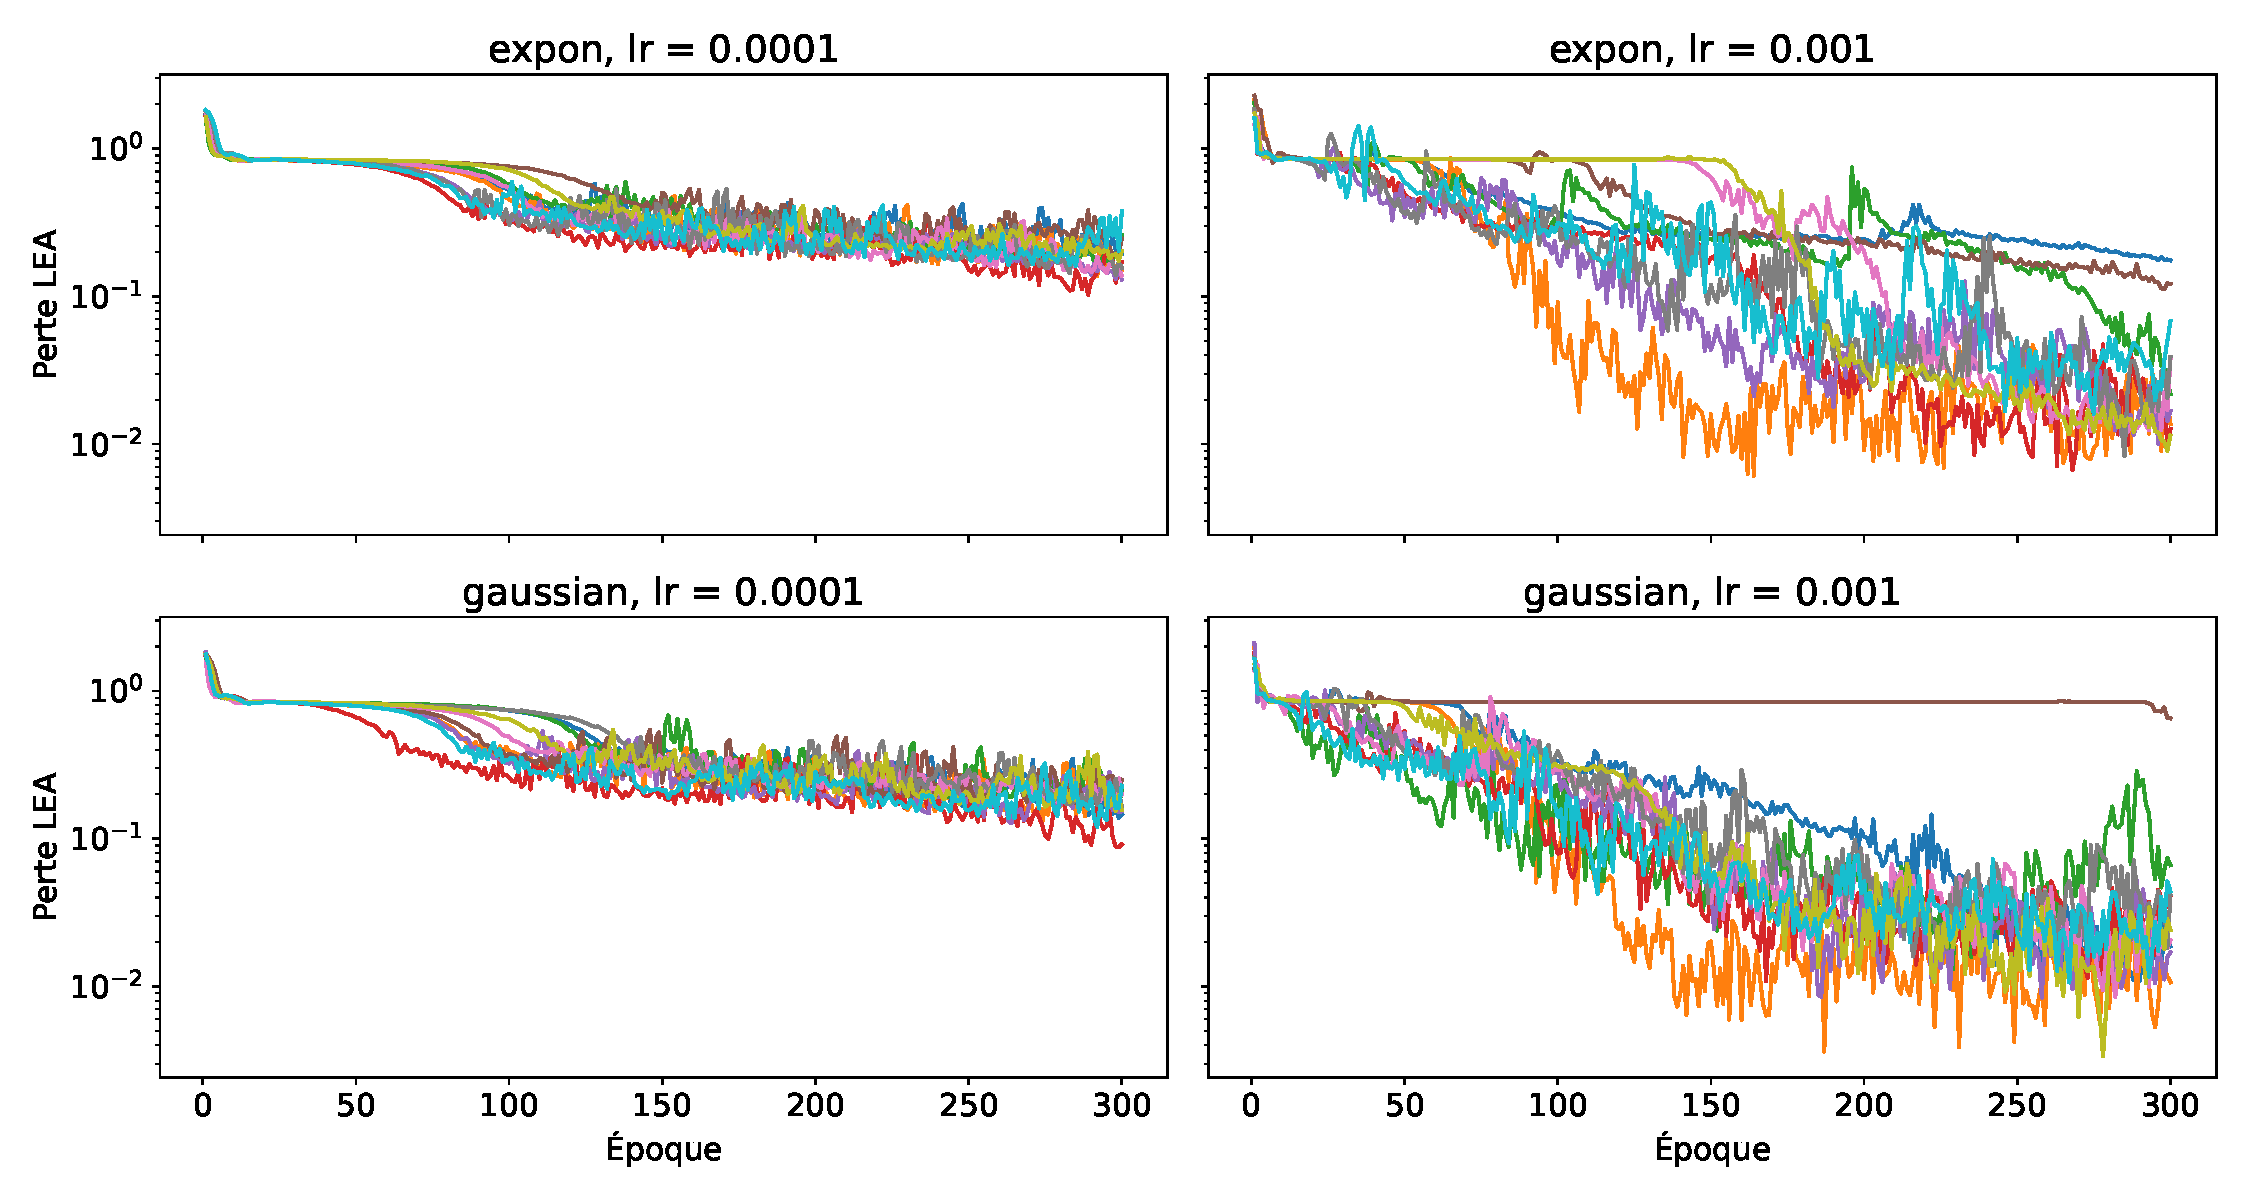
\includegraphics[width=1\linewidth]{images/all_losses_overfit_plus_petit.pdf}
    \caption{Graphiques des courbes d'entraînement pour les principaux paramètres physiques du régime $\tau_c < T$. Sur une même ligne, on compare l'effet du taux d'apprentissage.}
    \label{fig:allLossesOverfitPlusPetit}
\end{figure}
\begin{figure}[h!!]
    \centering
    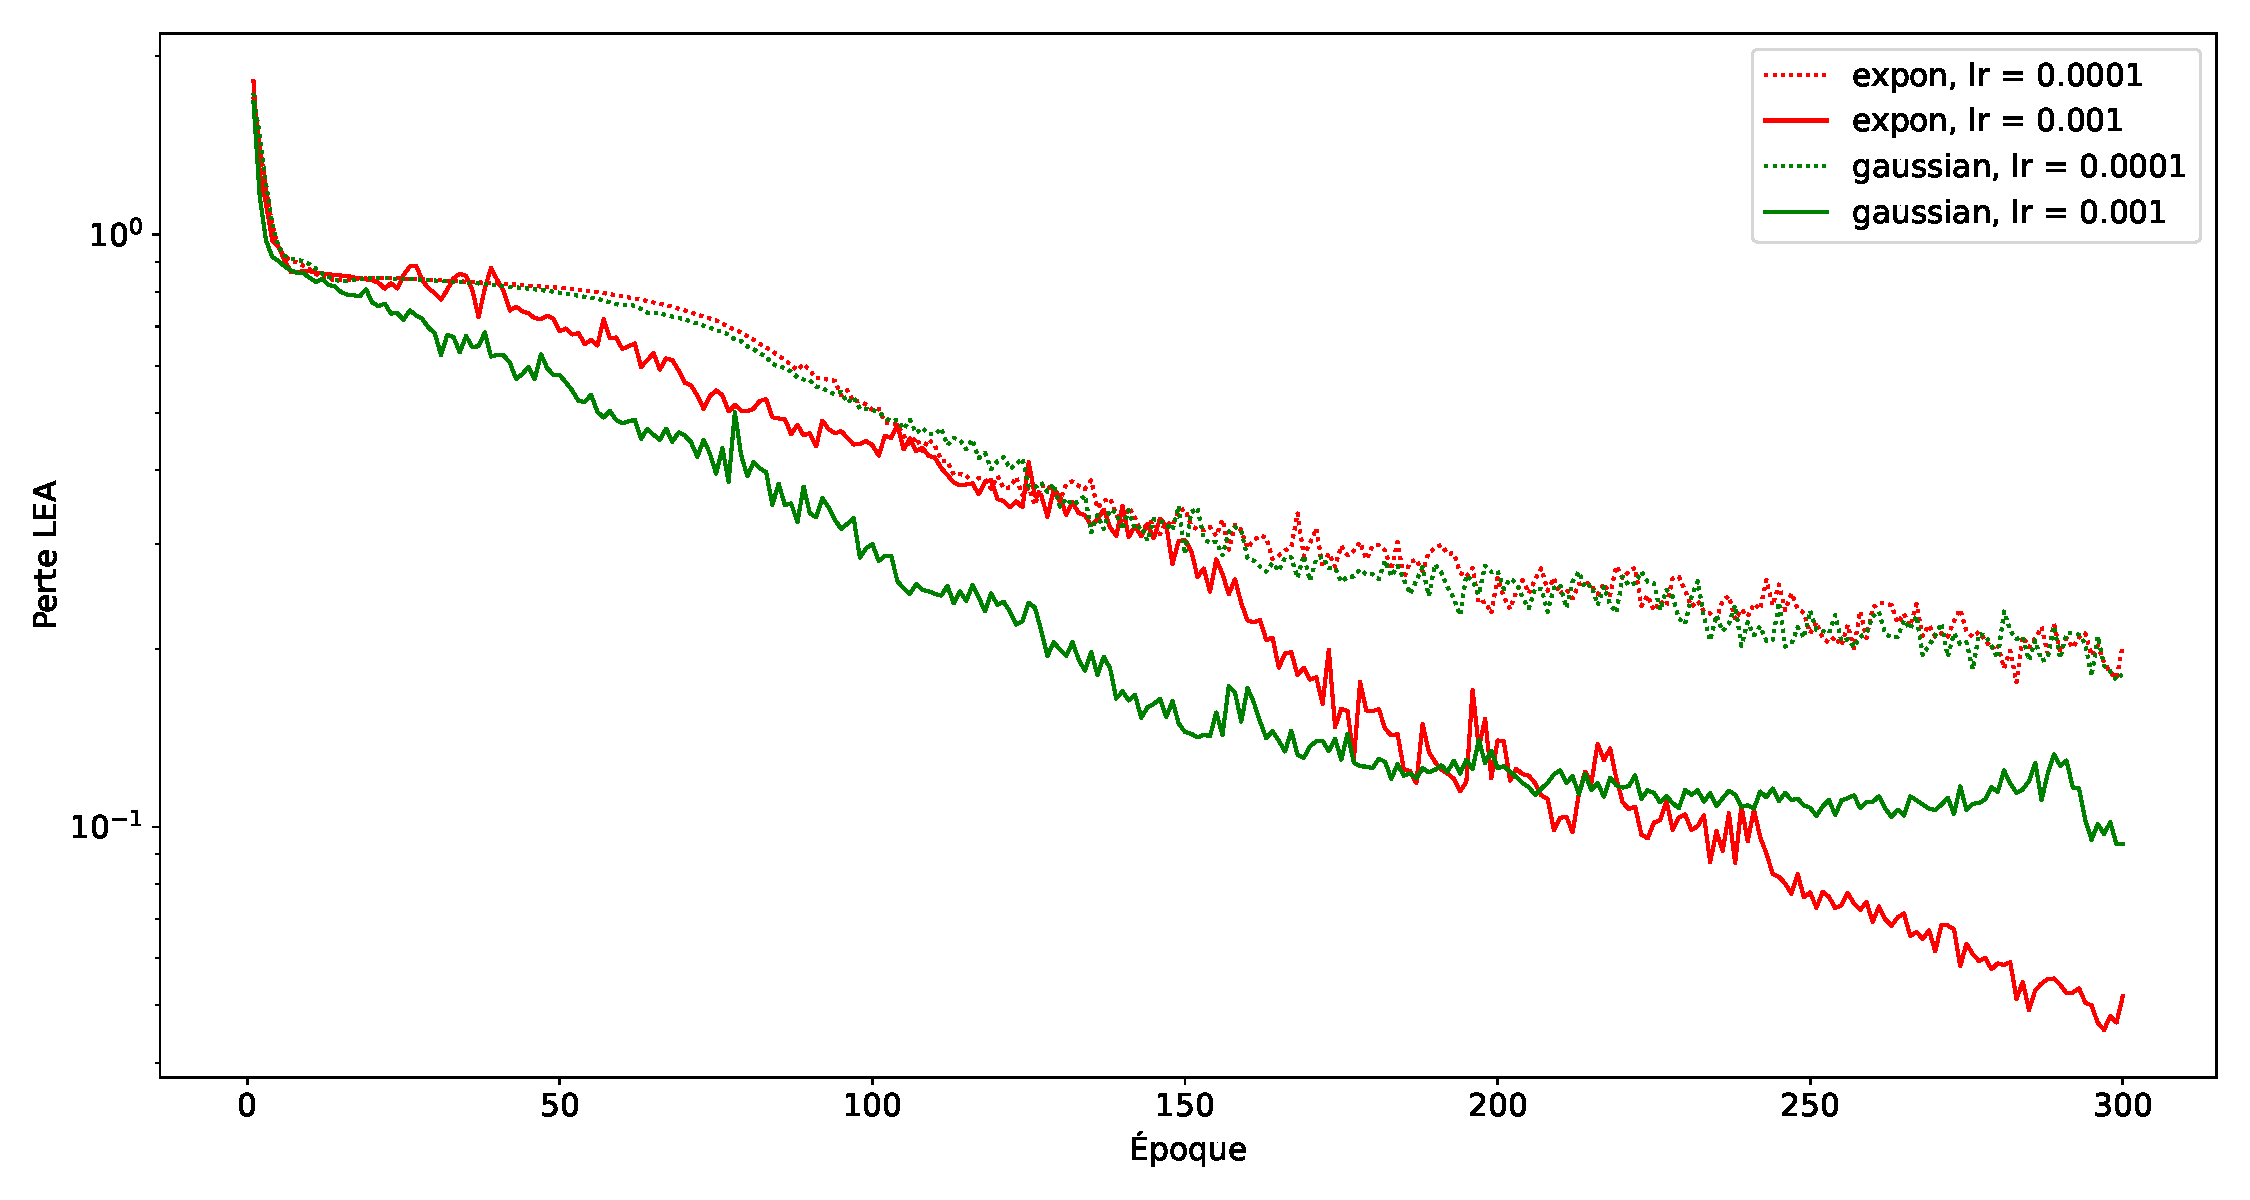
\includegraphics[width=0.9\linewidth]{images/moyennes_overfit_plus_petit.pdf}
    \caption{Moyennes des dix essais d'entraînement pour les quatre configurations importantes pour le régime $\tau_c < T$.}
    \label{fig:moyennesLossesOverfitPlusPetit}
\end{figure}
\newpage
Pour le régime $\tau_c \approx T$, on a aussi effectué dix entraînements avec les mêmes taux d'apprentissage, autant pour une corrélation exponentielle que gaussienne. Les dix courbes d'entraînement sont présentées à la figure \ref{fig:allLossesOverfitApprox}, alors que les moyennes sont présentées à la figure \ref{fig:moyennesLossesOverfitApprox}. On remarque une convergence rapide dans les quatre cas, mais aussi qu'un taux d'apprentissage plus petit serait mieux.
\begin{figure}[h!!]
    \centering
    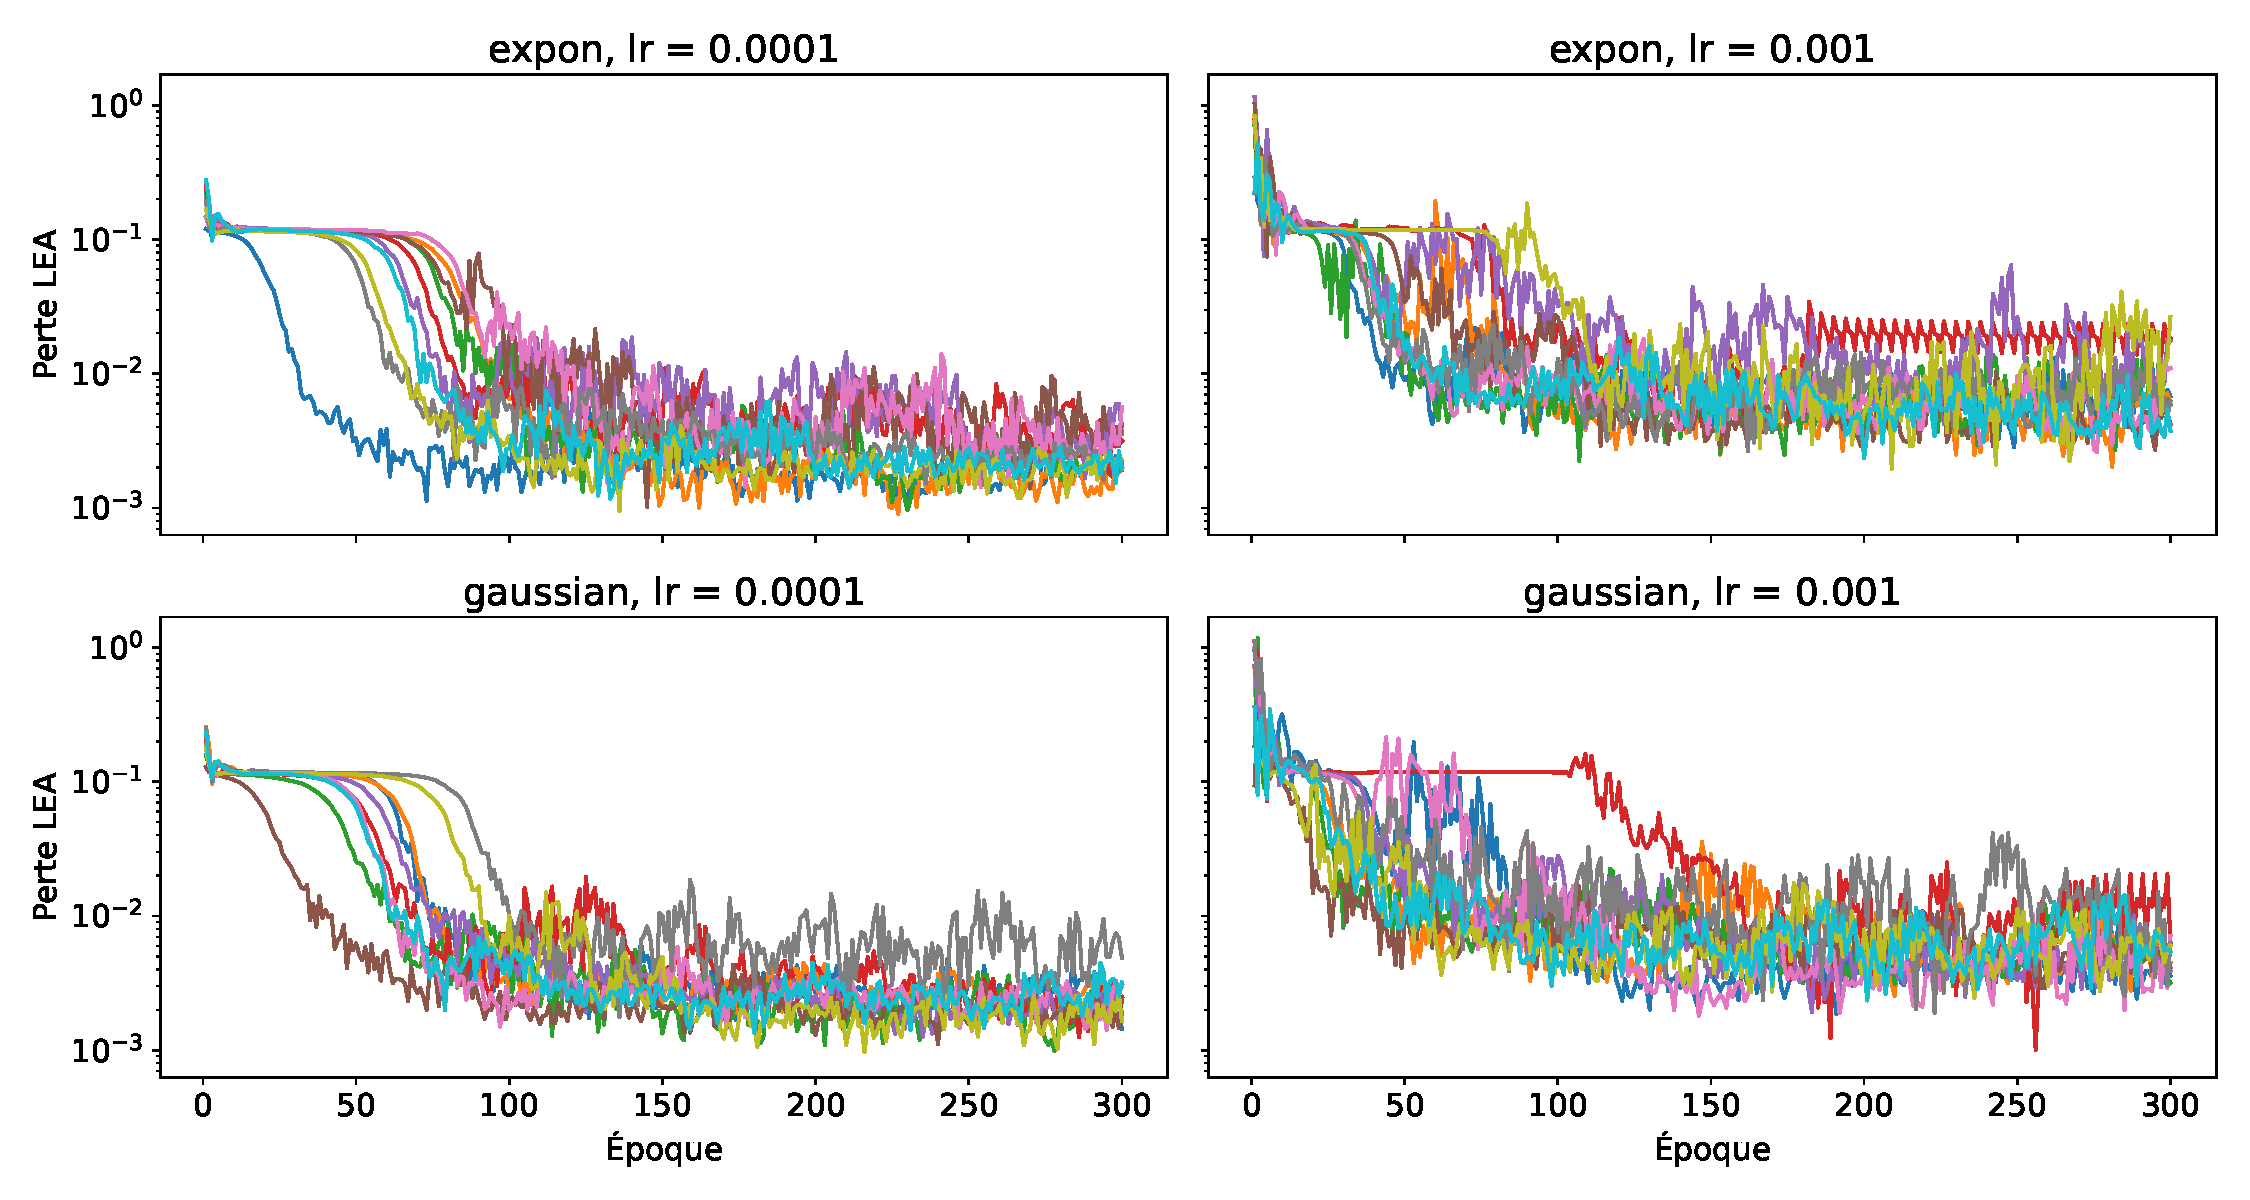
\includegraphics[width=1\linewidth]{images/all_losses_overfit_approx.pdf}
    \caption{Graphiques des courbes d'entraînement pour les principaux paramètres physiques du régime $\tau_c \approx T$. Sur une même ligne, on compare l'effet du taux d'apprentissage.}
    \label{fig:allLossesOverfitApprox}
\end{figure}
\begin{figure}[h!!]
    \centering
    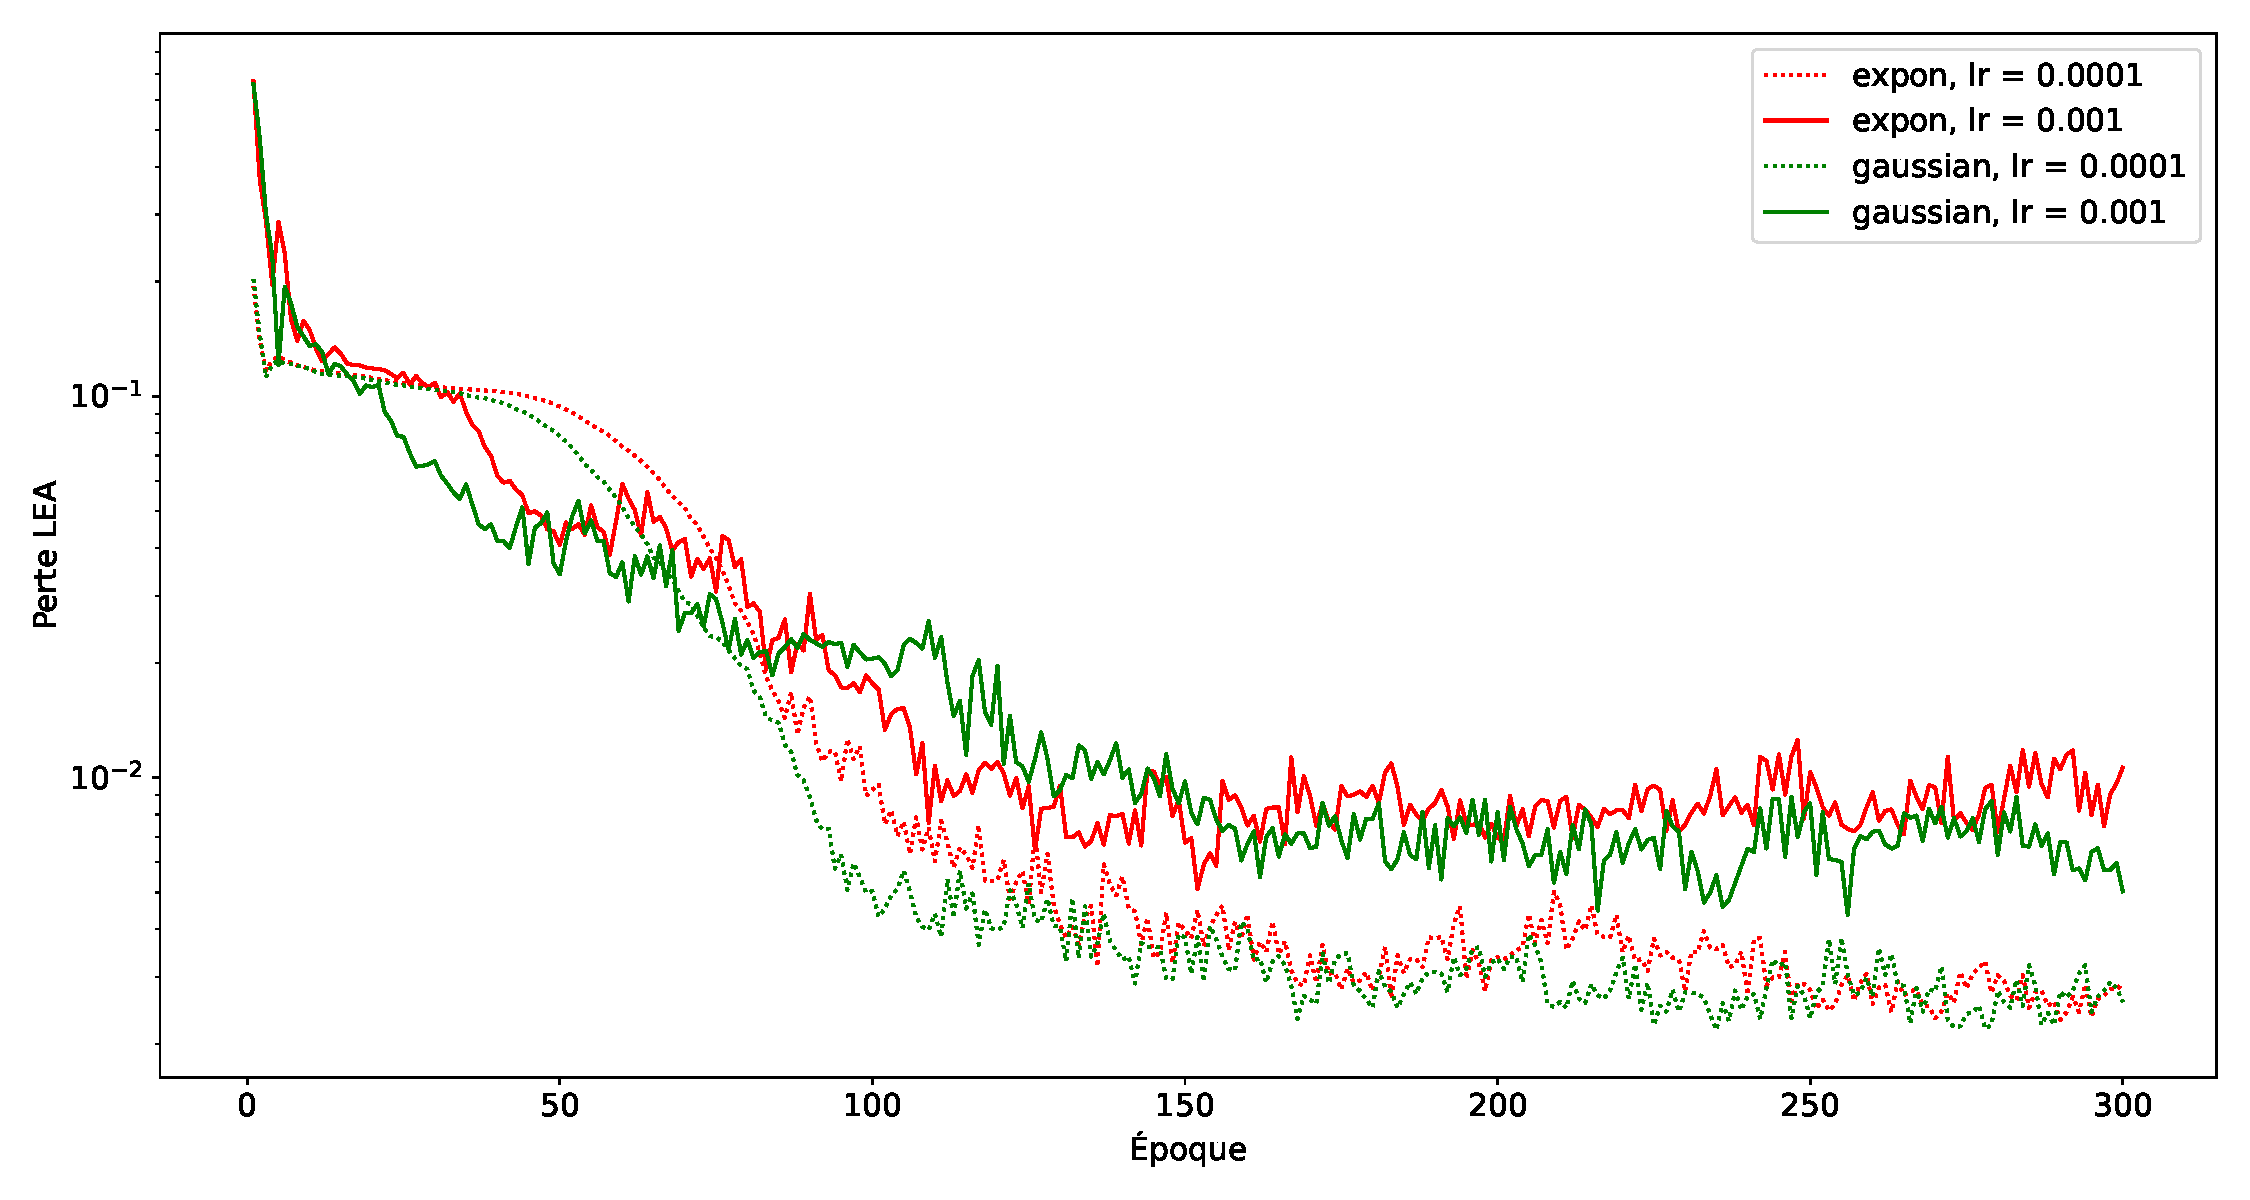
\includegraphics[width=0.9\linewidth]{images/moyennes_overfit_approx.pdf}
    \caption{Moyennes des dix essais d'entraînement pour les quatre configurations importantes pour le régime  $\tau_c \approx T$.}
    \label{fig:moyennesLossesOverfitApprox}
\end{figure}
\newpage
Finalement, les courbes des dix entraînement du régime $\tau_c > T$ sont présentées à la figure \ref{fig:allLossesOverfitPlusGrand} et la figure \ref{fig:moyennesLossesOverfitPlusGrand} présente les moyennes. Les courbes sont similaires à celles du régime précédent, notamment avec un taux de $10^{-4}$ plus efficace sur le long terme.
\begin{figure}[h!!]
    \centering
    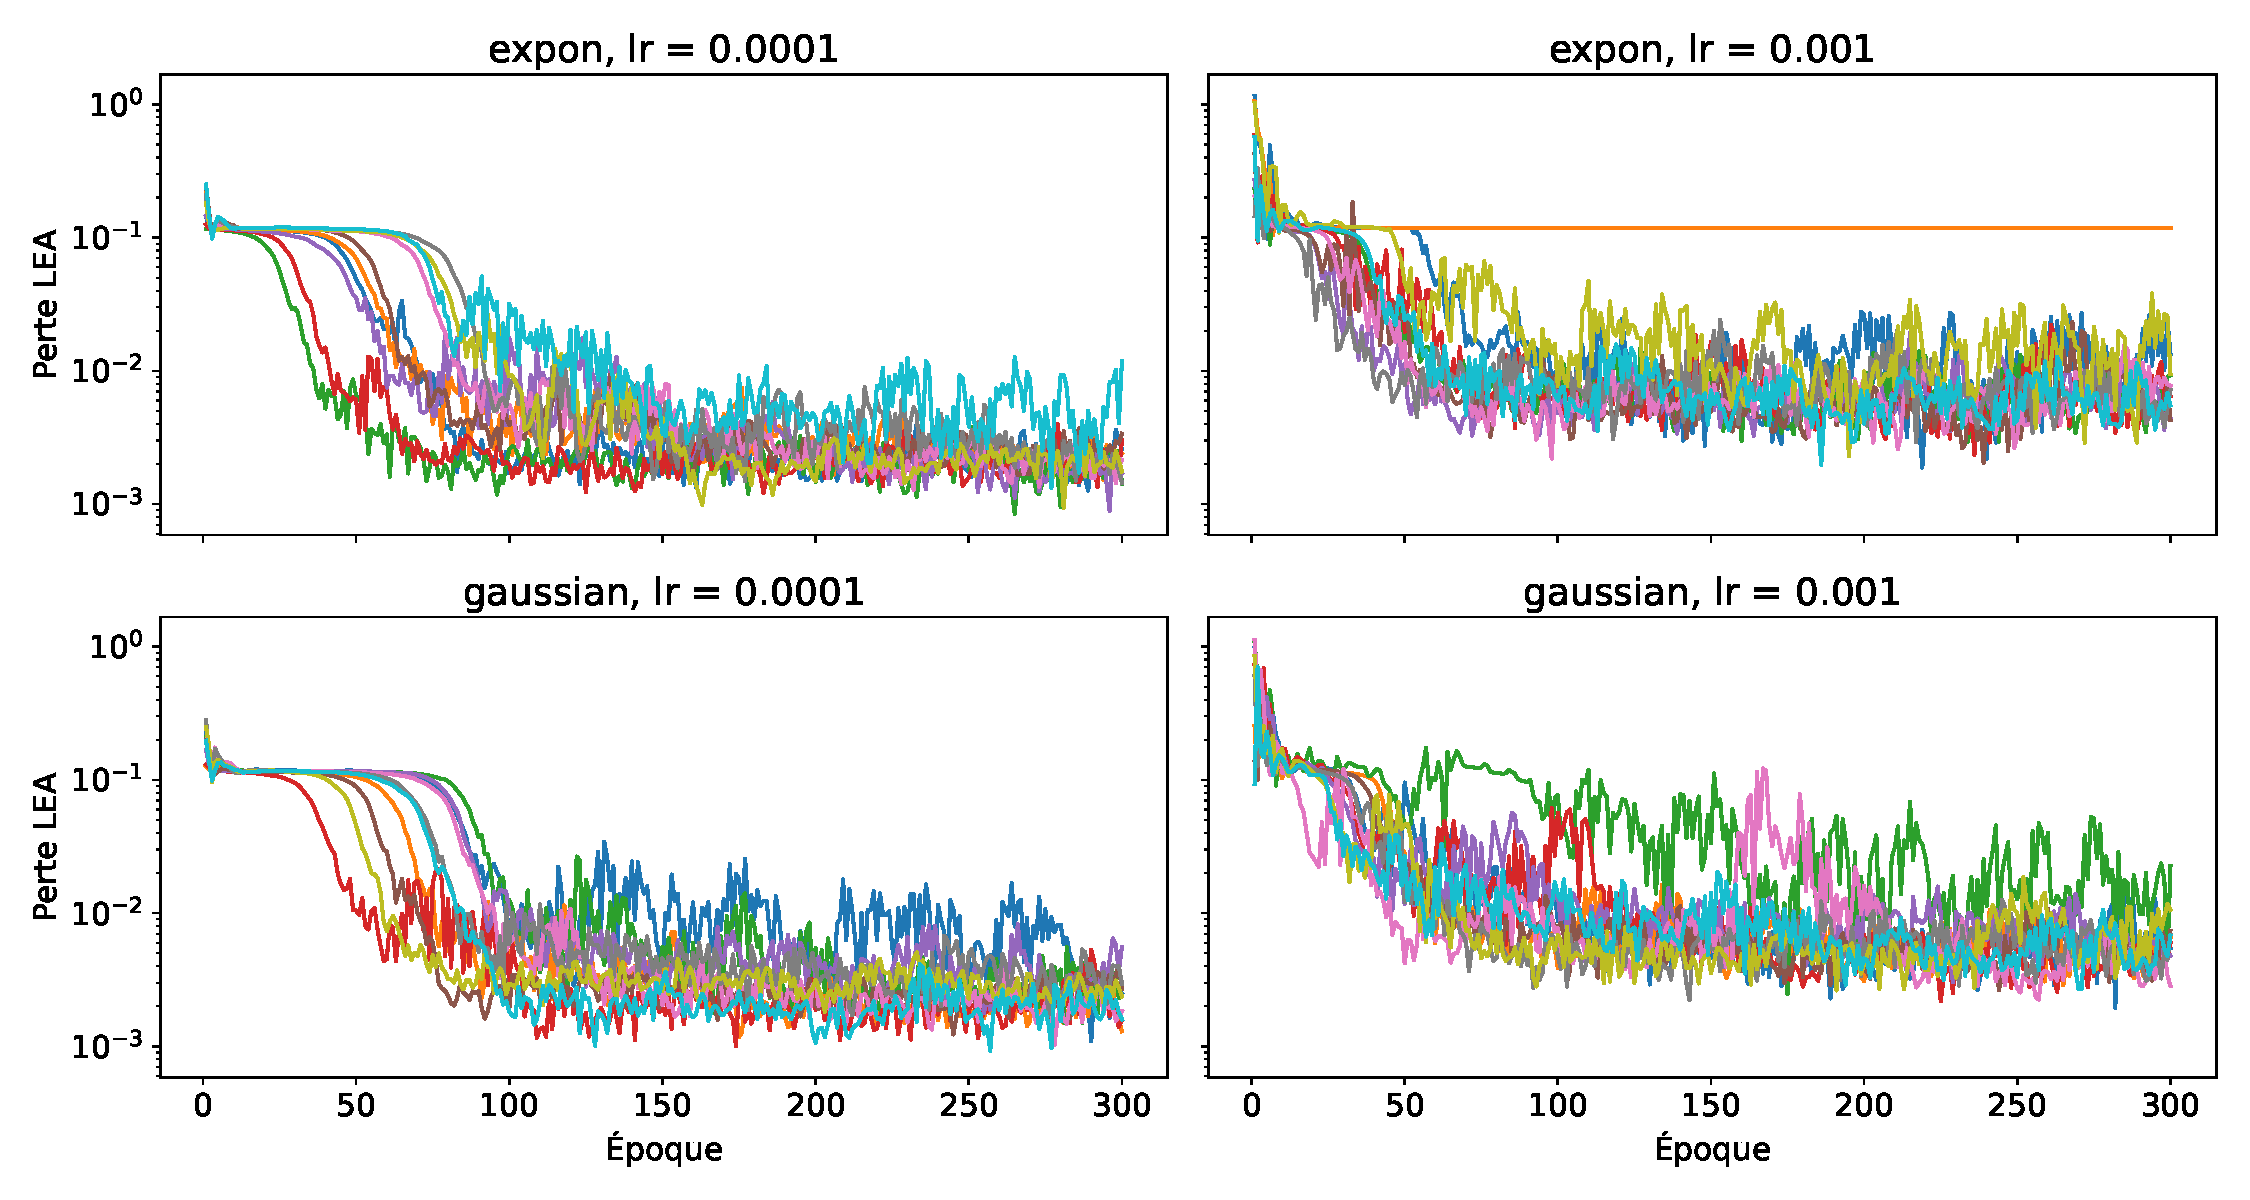
\includegraphics[width=1\linewidth]{images/all_losses_overfit_plus_grand.pdf}
    \caption{Graphiques des courbes d'entraînement pour les principaux paramètres physiques du régime $\tau_c > T$. Sur une même ligne, on compare l'effet du taux d'apprentissage.}
    \label{fig:allLossesOverfitPlusGrand}
\end{figure}
\begin{figure}[h!!]
    \centering
    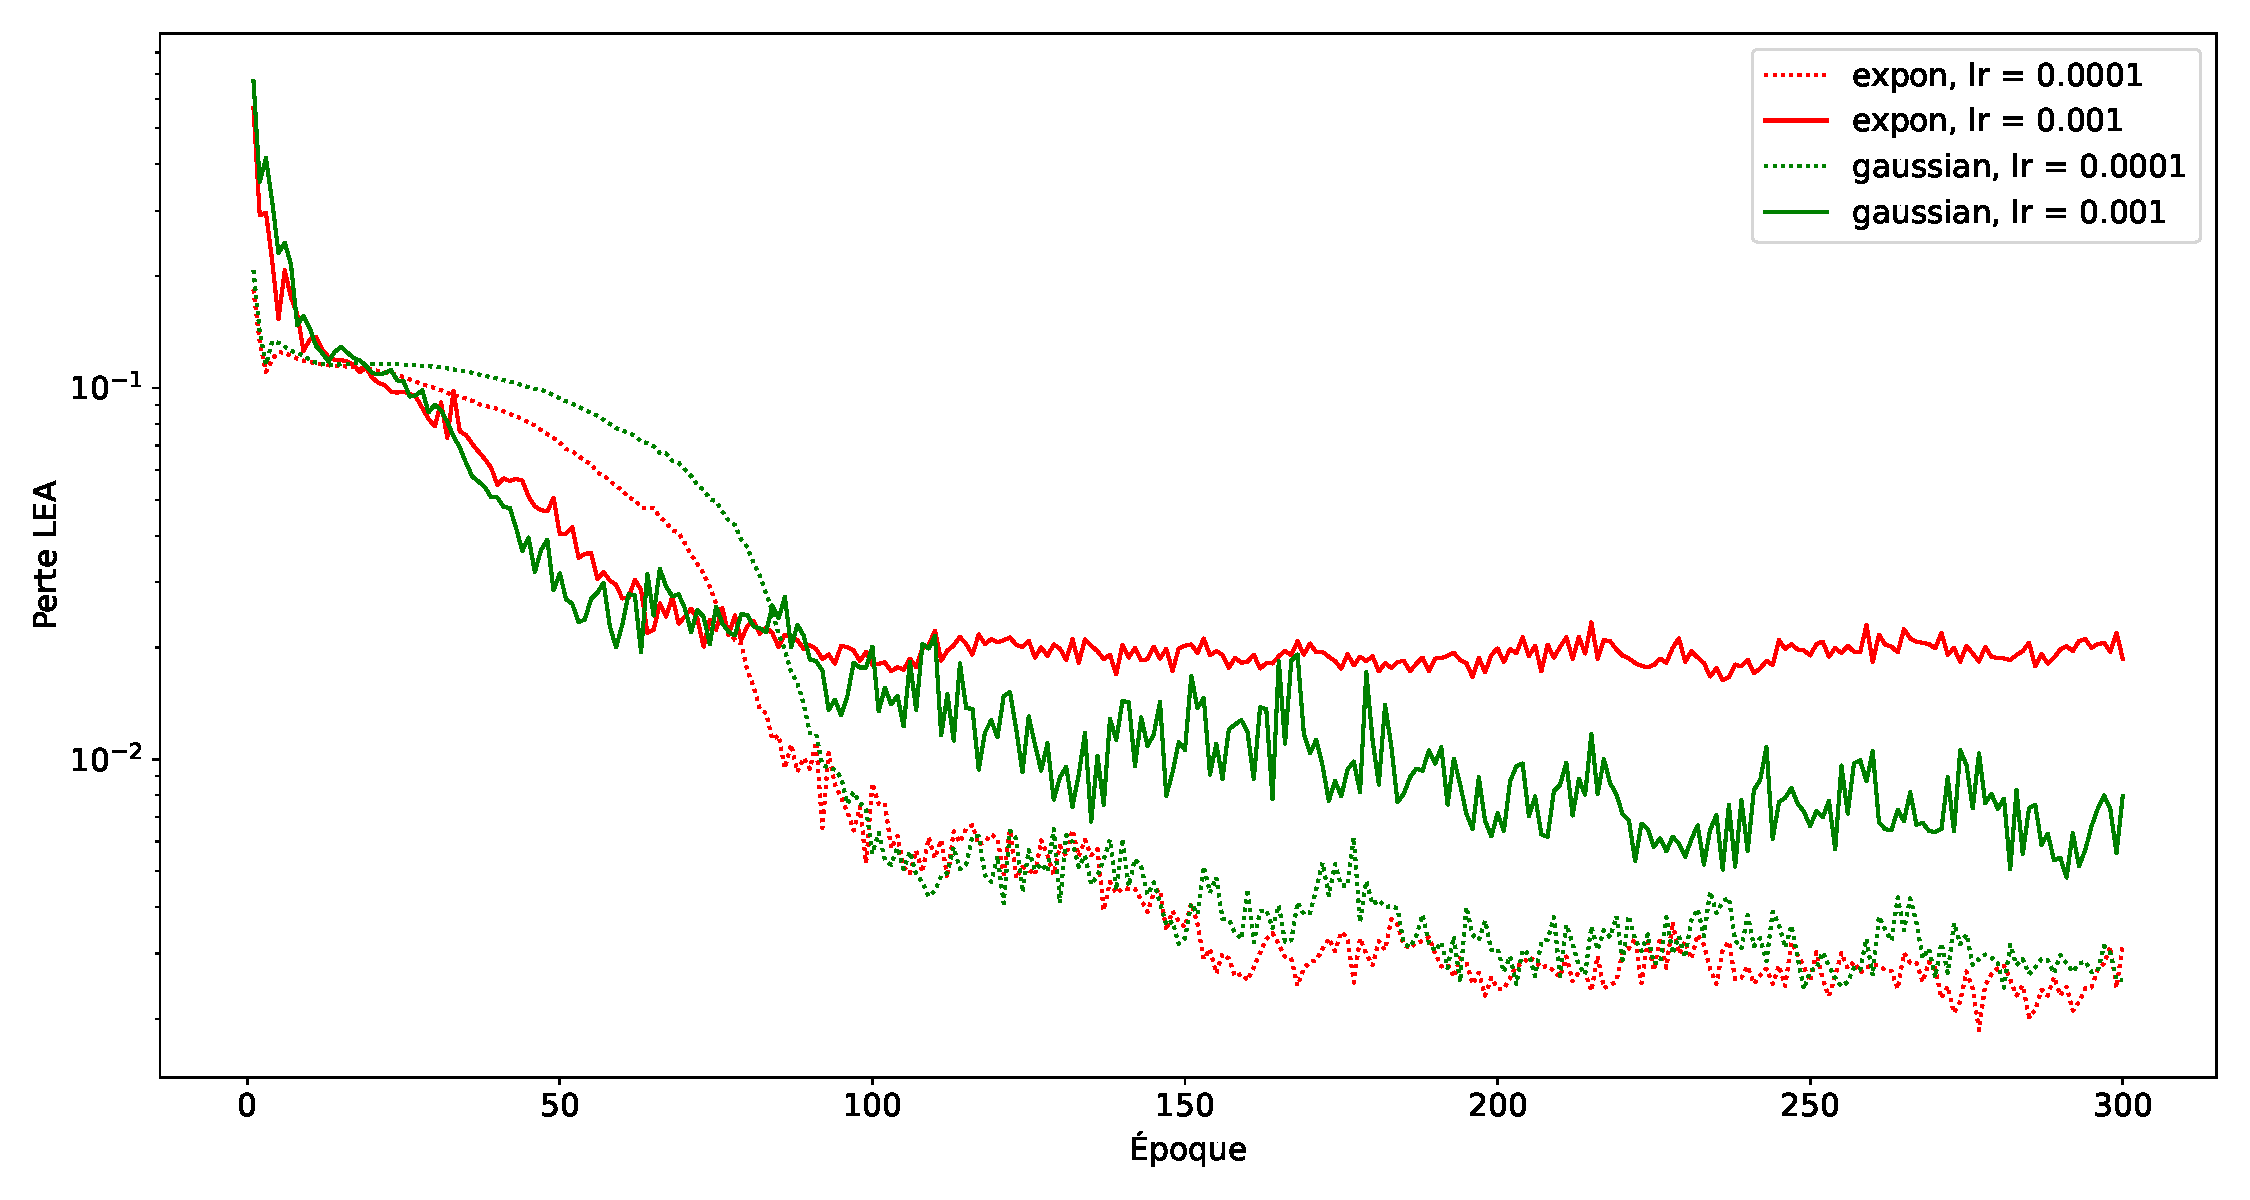
\includegraphics[width=0.9\linewidth]{images/moyennes_overfit_plus_grand.pdf}
    \caption{Moyennes des dix essais d'entraînement pour les quatre configurations importantes pour le régime  $\tau_c > T$.}
    \label{fig:moyennesLossesOverfitPlusGrand}
\end{figure}
\newpage
Finalement, il est aussi pertinent de vérifier si un taux d'apprentissage de $10^{-2}$ serait viable. On a alors expérimenté avec le régime $\tau_c < T$, car c'est lui qui pourrait bénéficier d'un taux d'apprentissage plus élevé. On a alors entraîné sur $200$ époques pour le même nombre de données et pour dix essais indépendants. La figure \ref{fig:overfitPlusPetit_mauvais} montre les dix courbes d'entraînement, ainsi que la moyenne. Il est évident par la figure que ce taux d'entraînement n'est pa à utiliser, du moins sur toutes les époques. On plafonne rapidement à une perte autour de $0.85$, ce qui n'est pas optimal comparativement aux taux plus petits utilisés précédemment.
\begin{figure}[h!!]
    \centering
    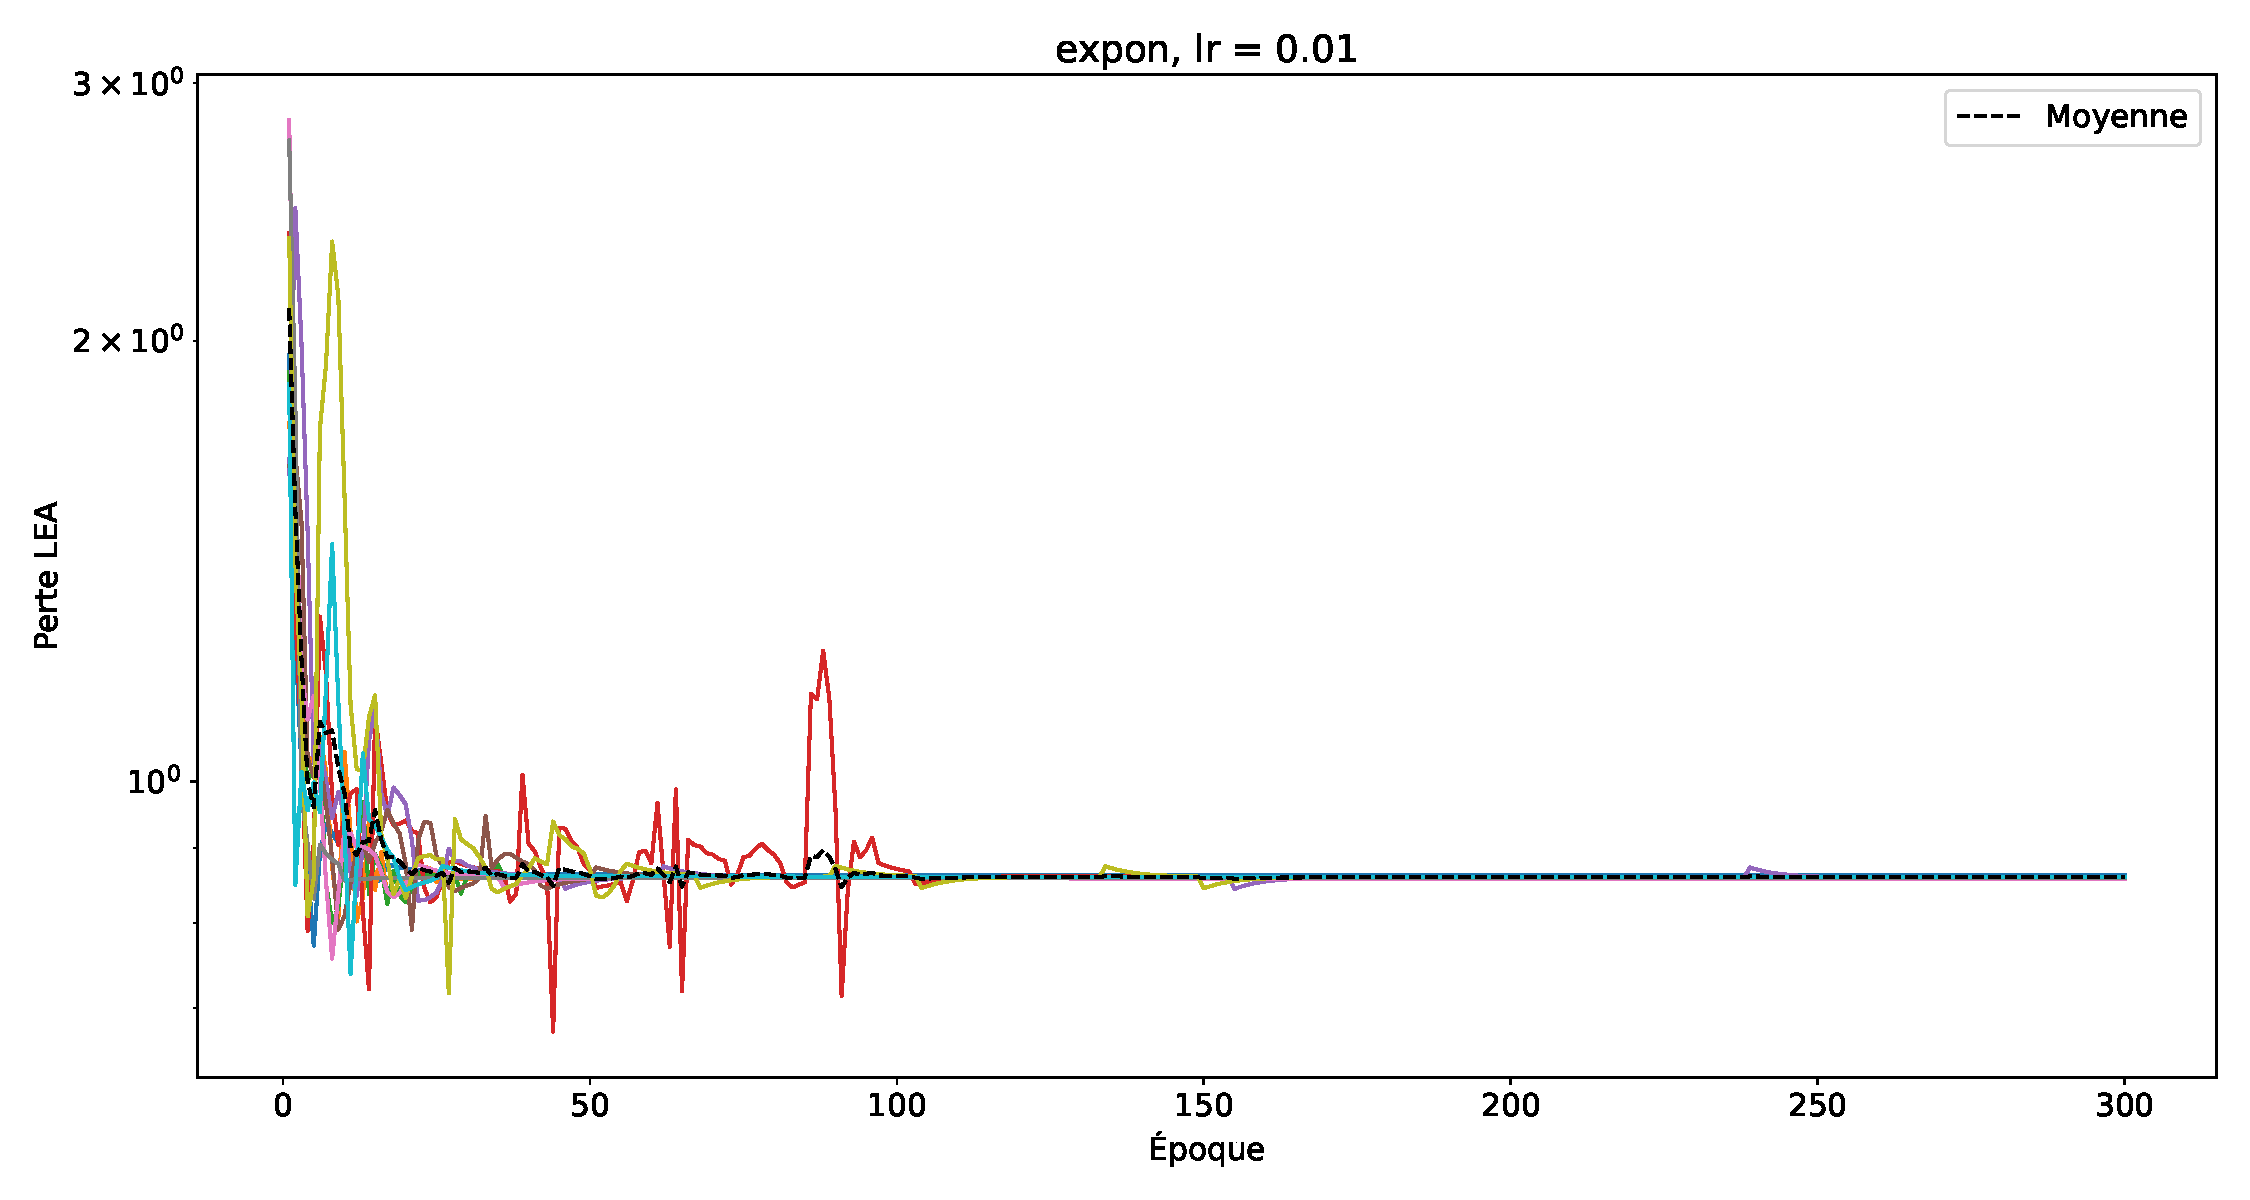
\includegraphics[width=0.9\linewidth]{images/plus_petit_0p01_overfit.pdf}
    \caption{Courbes et moyenne des dix essais d'entraînement dans le régime $\tau_c < T$ pour un taux d'apprentissage de $10^{-2}$ et une corrélation exponentielle.}
    \label{fig:overfitPlusPetit_mauvais}
\end{figure}
En terminant ce chapitre, il est pertinent de parler de l'interprétation de la perte $LEA$, soit la log erreur absolue. Pour rappel, si $\tau_c$ est le vrai temps caractéristique et $\hat{\tau}_c$ est l'estimation du réseau, la perte $LEA$ est définie comme:
\begin{align*}
LEA = \abs{\log\hat{\tau}_c - \log\tau_c} = \abs{\log\left(\frac{\hat{\tau}_c}{\tau_c}\right)}
\end{align*}
et on peut revenir à l'échelle naturelle avec:
\begin{align*}
E = \exp{\pm LEA}
\end{align*}
où $E$ est l'erreur multiplicative entre $\hat{\tau}_c$ et $\tau_c$. Par exemple, si on a $LEA = 1$, on a $E = \exp{\pm1}$, donc l'erreur multiplicative est soit d'environ $2.72$ ou $0.37$, donc que $\frac{\hat{\tau}_c}{\tau_c} \approx 2.72$ ou $\frac{\hat{\tau}_c}{\tau_c} \approx 0.37$. Dans les cas présentés jusqu'ici, on arrive presque tout le temps à des pertes finales sous $10^{-1}$ (voire $10^{-2}$), ce qui donne des erreurs multiplicatives de moins de $\exp{\pm 0.1}$, soit entre $0.9$ et $1.1$. Si on prend un $\tau_c$ de $0.5$, on a alors une estimation dans l'intervalle $[0.45, 0.55]$, ce qui est très bien pour un intervalle conservateur compte tenu de la complexité stochastique des tavelures laser. Le réseau est capable d'apprendre une petite séquence. Il faut maintenant tester l'entraînement et la validation sur un jeu de données complet.
\newpage
\chapter{Résultats initiaux}
\label{resultats_initiaux}
Ce chapitre présente les principaux résultats d'entraînement obtenus durant la première partie du projet. Dans tous les cas présentés, on utilise le réseau schématisé à la figure \ref{fig:schema_v1}, mais avec des hyperparamètres différents. Le code utilisé dans le cadre de ce projet est disponible sur le GitHub public \url{https://github.com/GabGabG/ProjetIntegrateur-DESS} en constante évolution. À noter que les données, qui sont en grande quantité, ne sont que sur Valéria et peuvent être rendues diponibles si besoin.
\section{Jeux de données}
Pour ce chapitre, deux jeux de données sont utilisés, simulés selon ce qui est présenté au chapitre \ref{donnees}. Premièrement, un lot de $500$ séquences temporelles de $50$ images $128\times128$ est généré. Dans ces simulations, on a des tavelures de largeur moyenne de $3$ pixels et des temps de corrélations variant en logarithme entre $10^{-2}$ et $10$, pour un temps d'intégration de $1$ (toutes ces unités sont arbitraires, tant qu'elles sont les mêmes). Échantillon $100$ valeurs de $\tau_c$ uniformément dans l'espace logarithmique et génère $5$ séquences ayant le même $\tau_c$, d'où la taille finale de $500$ séquences. La fonction de corrélation est restée constante à la fonction exponentielle.
\\ \\
Deuxièmement, un lot de $5000$ séquences temporelles de $50$ images $128\times 128$ est généré. Les tavelures sont aussi de largeur moyenne de $3$ pixels, avec des temps de corrélations dans le même espace logarithmique. Par contre, on échantillonne $1000$ valeurs différentes de $\tau_c$ avec encore une fois $5$ répétitions par $\tau_c$, donnant $5000$ séquences. Le temps d'intégration et la fonction de corrélation n'ont pas changés.
\section{Premier réseau}
Le premier réseau est composé d'un CNN ayant trois couches, chacune donnant respectivement une carte de caractéristique de $16$, $32$ et $64$ canaux. Chaque couche est composée d'un noyau $3\times3$, suivi d'une activation ReLU. On applique un rembourrage des images avec un mode de réflection, permettant de garder la taille initiale des images. Le mode de réflection est choisi pour ne pas tenir compte de données fausses, comme le mode constant, et est logique avec la nature stochastique des tavelures, permettant de répéter les motifs par réflexion. À la fin du CNN, on applique une convolution $1x1$ permettant de ramener le nombre de canaux à $1$, et on passe le tout dans une couche linéaire diminuant le nombre de caractéristiques à $64$ par image, permettant une sorte d'attention spatiale pouvant apprendre.\\ \\
Pour la partie récurrente, en plus des $64$ caractéristiques par images, on en ajoute une: le temps d'intégration. On donne ces caractéristiques à un GRU unidirectionnel d'une couche et $128$ unités cachées. Le tout donne au final un scalaire, soit le logarithme naturel du temps caractéristique de corrélation estimé. À la figure \ref{fig:learning_curves_v1}, on montre les courbes d'apprentissage pour ce réseau. On a utilisé le jeu de $500$ séquences temporelles de $50$ images, séparées en données d'entraînement ($80\%$) et de validation ($20\%$). L'apprentissage se fait par mini lots de taille $8$ et à l'aide d'un otpimiseur Adam auquel on spécifie un taux d'apprentissage de $10^{-4}$ qui reste constant. On note un fort sur-apprentissage, car la perte en validation atteint rapidement un plateau. Le second réseau sera modifié pour tenter de cibler la cause de la mauvaise généralisation.
\begin{figure}[h!!]
    \centering
    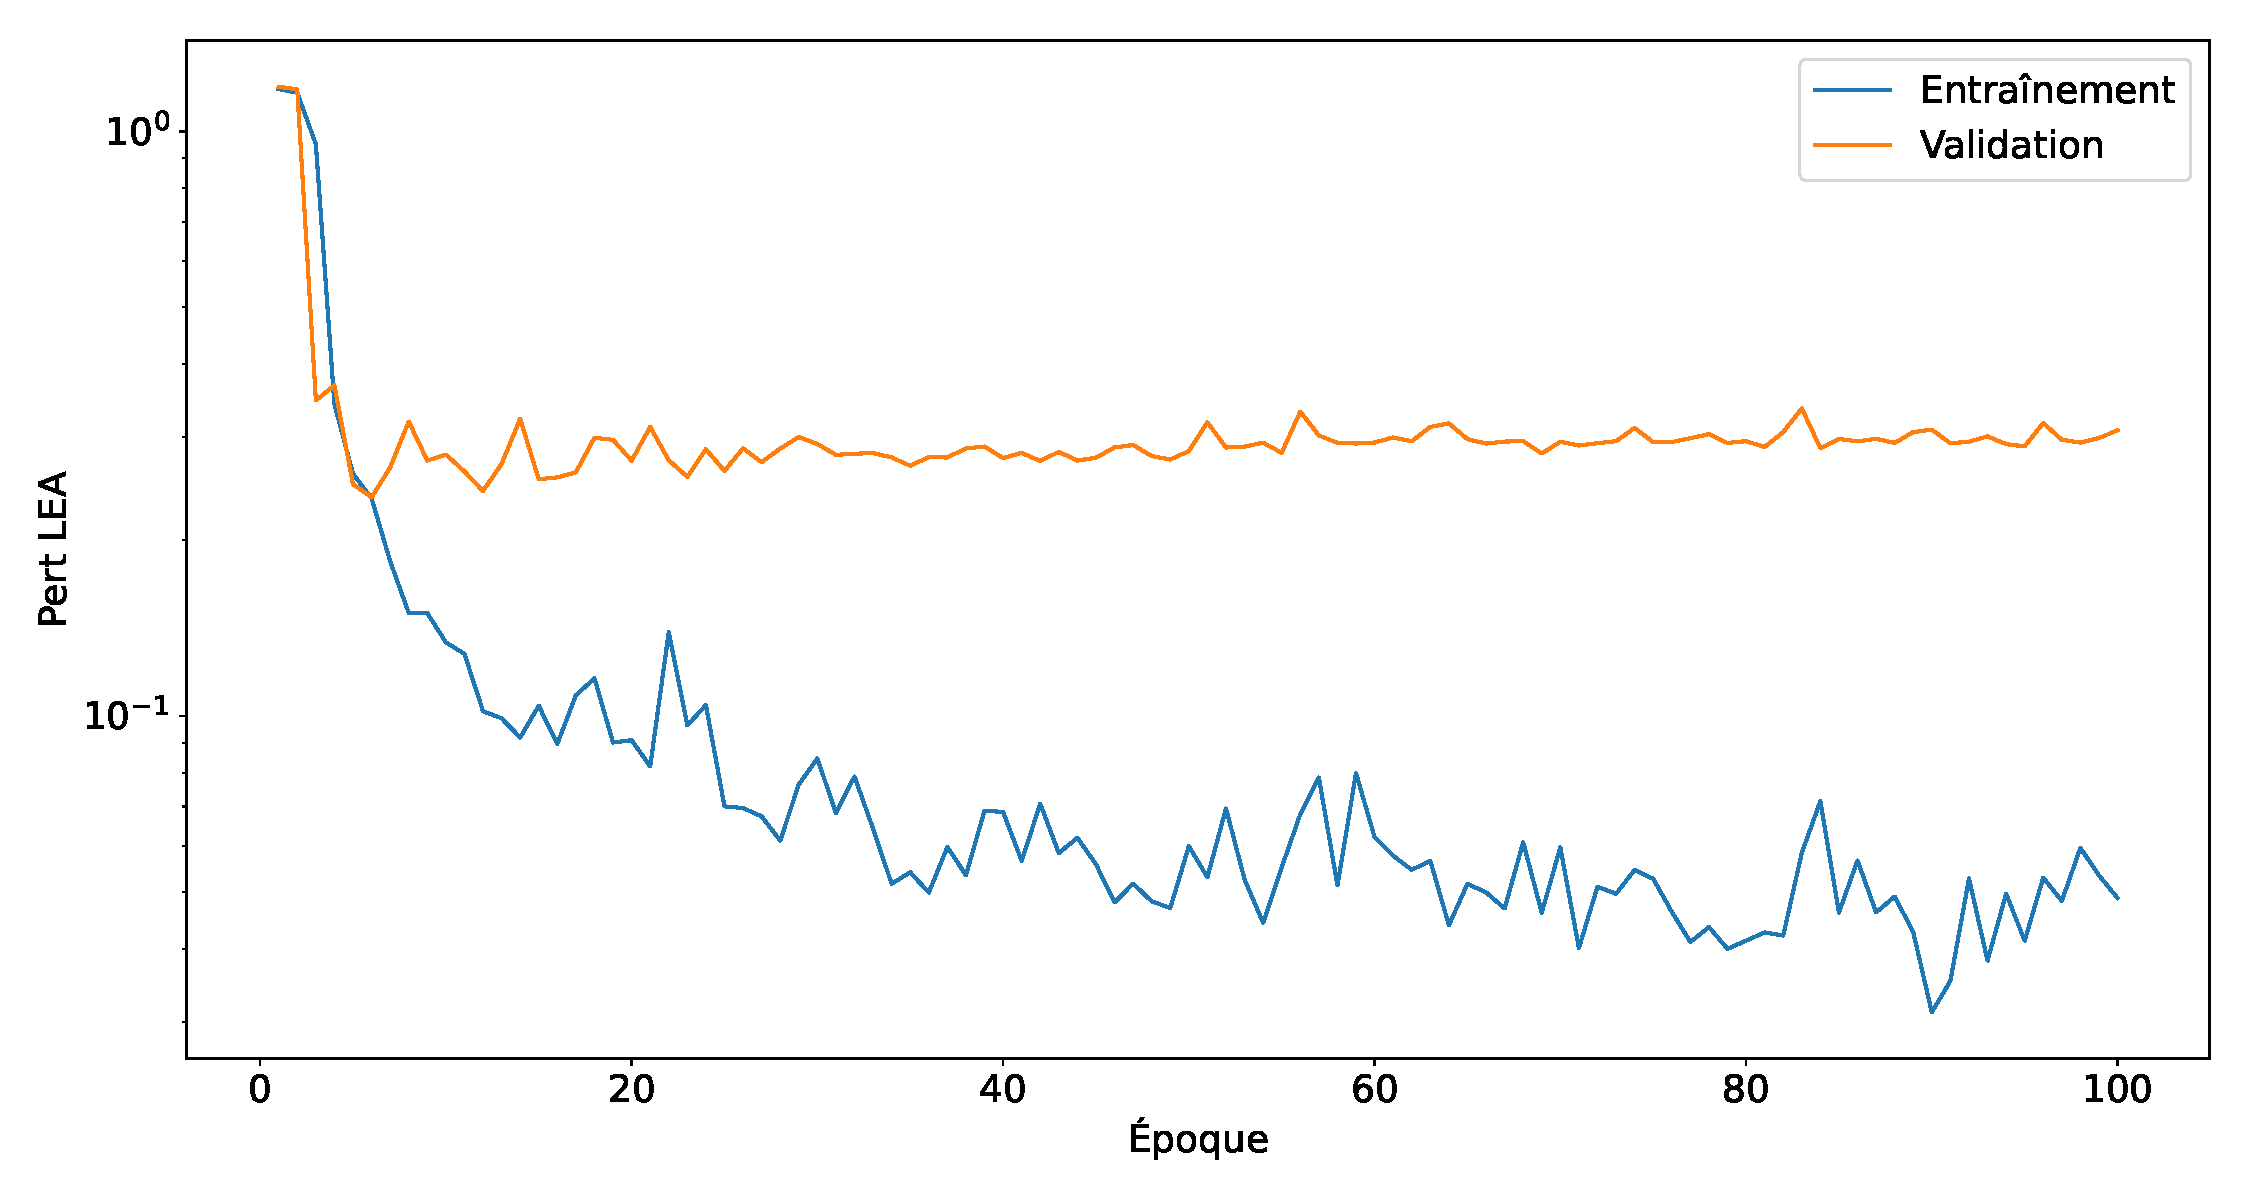
\includegraphics[width=1\linewidth]{images/learning_curves_v1.pdf}
    \caption{Courbes d'entraînement et de validation pour le premier réseau. On entraîne sur $100$ époques.}
    \label{fig:learning_curves_v1}
\end{figure}
\newpage
\section{Deuxième réseau}
Le second réseau diffère du premier dans le nombre de cannaux et de couches du CNN, du nombre de neurones dans la partie linéaire d'attention et dans le nombre d'unités cachées du GRU. On a deux couches CNN, toutes deux avec $8$ canaux de sortie. Pour la couche linéaire, on a $32$ sorties au lieu de $64$. Le GRU contient $64$ unités cachées. Le but de ce réseau est de vérifier si le premier réseau était trop complexes pour les données, donc favorisait le sur-apprentissage. On garde le même nombre de mini lots et le même optimiseur Adam avec un taux d'apprentissage de $10^{-4}$, et on entraîne sur les même séquences. La figure \ref{fig:learning_curves_v2} montre les courbes d'entraînement pour ce réseau. On remarque des performances similaires, quoique légèrement meilleures avec un plateau plus tard et plus bas, ainsi qu'avec un sur-apprentissage plus lent à démarrer. Cela laisse croire que le modèle peut être rétrécie sans rendre l'apprentissage plus difficile.
\begin{figure}[h!!]
    \centering
    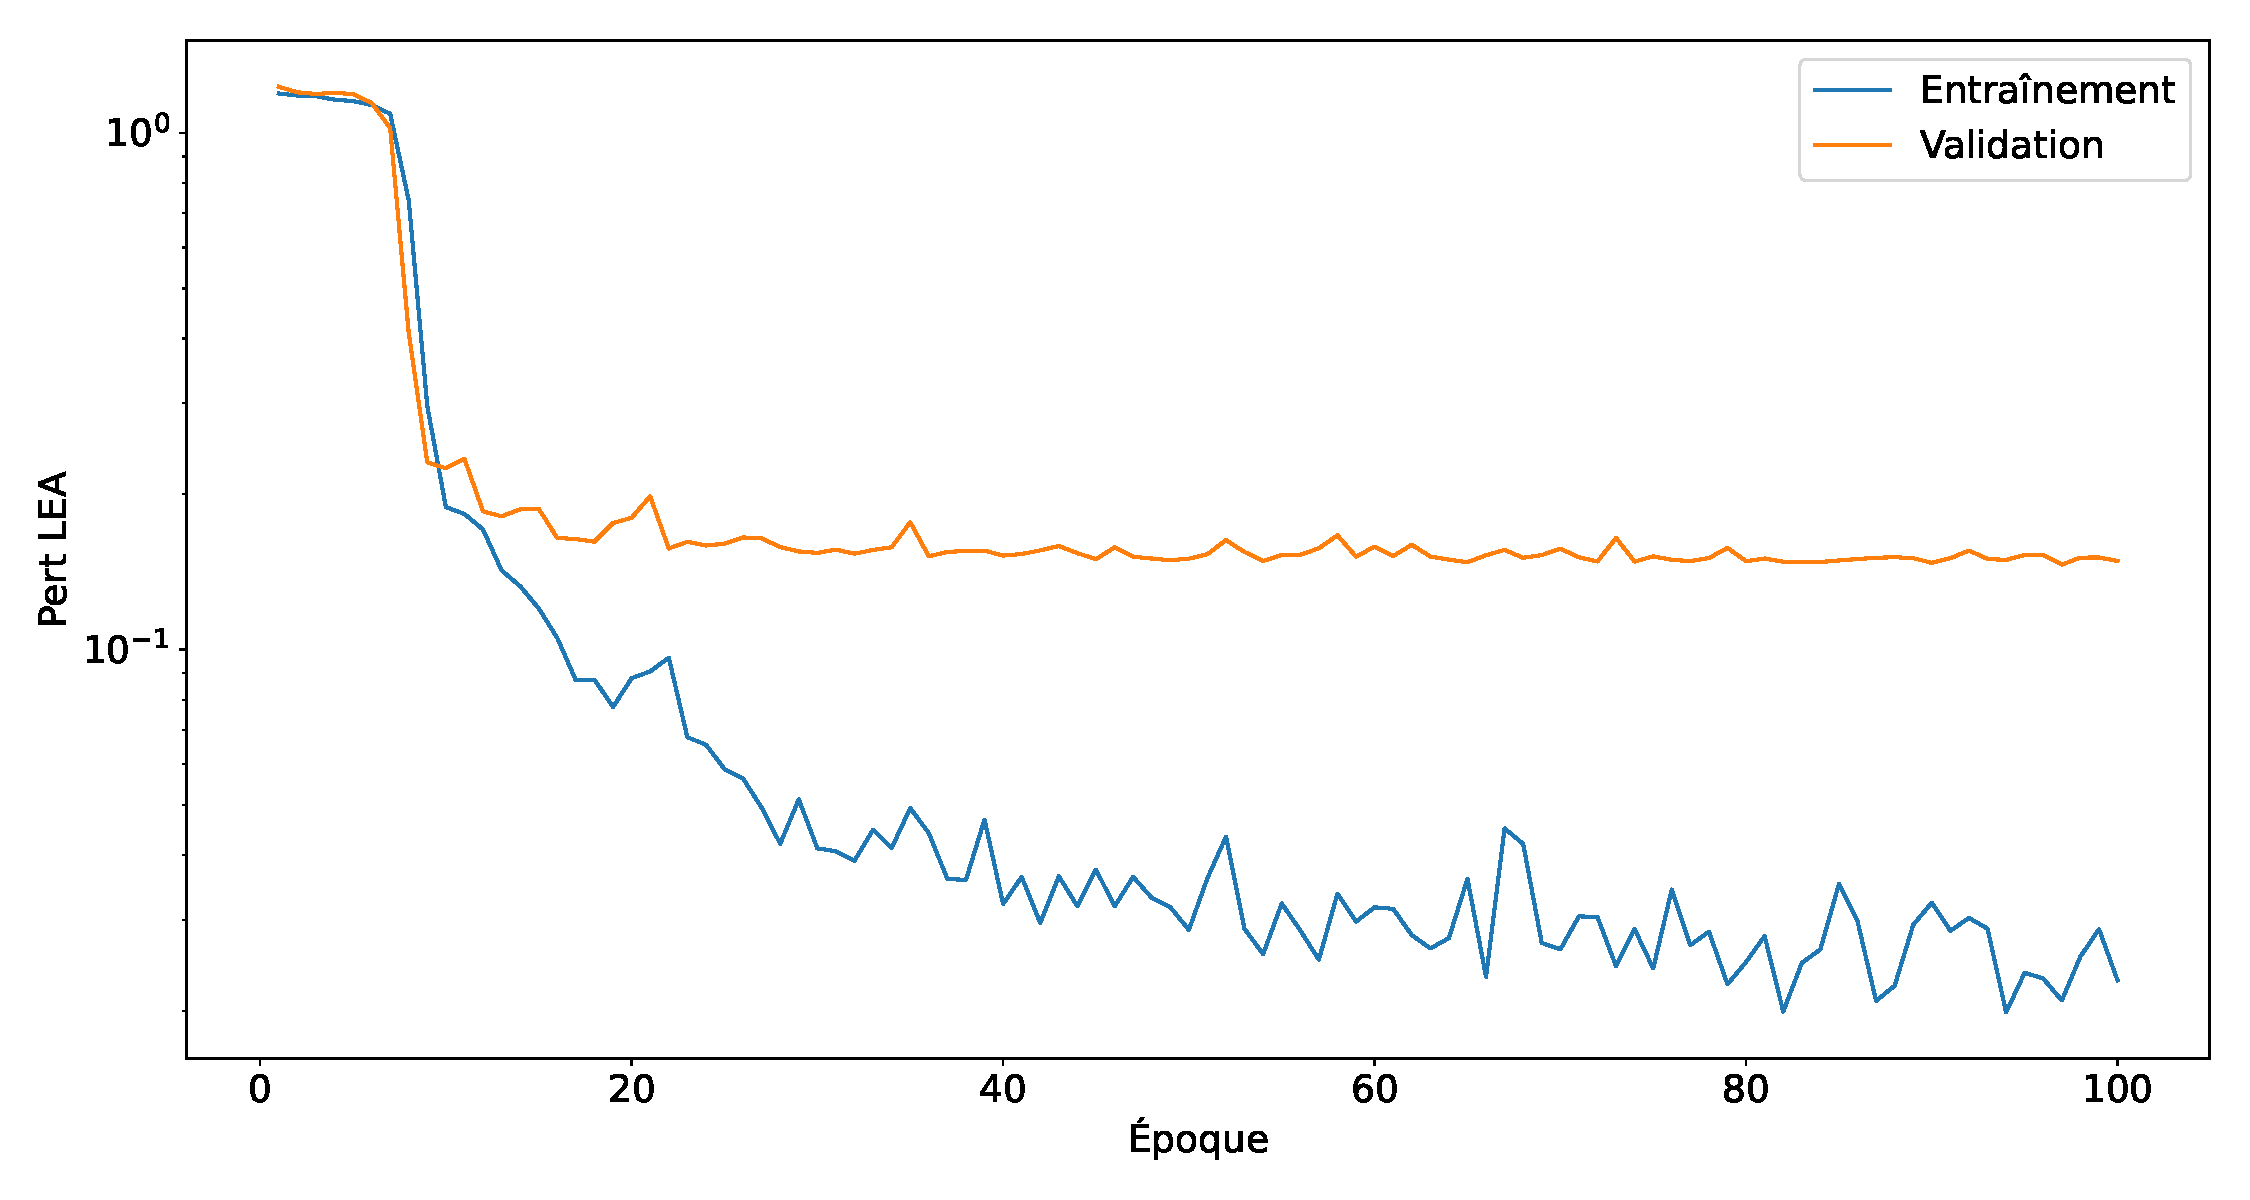
\includegraphics[width=1\linewidth]{images/learning_curves_v2.pdf}
    \caption{Courbes d'entraînement et de validation pour le deuxième réseau. On entraîne sur $100$ époques.}
    \label{fig:learning_curves_v2}
\end{figure}
\section{Troisième réseau}
Le troisième réseau est aussi une légère réduction du premier. On a une fois de plus deux couches, comme le second, mais cette fois les canaux sont $8$, puis $16$. On ne change pas l'attention ni le GRU. Par contre, on utilise le jeu de $5000$ données. Une possible explication des mauvaises performances des deux premiers est le manque de données. Étant donné la nature stochastique des tavelures, un plus grand nombre de données pourrait apporter une bonne amélioration. On utilise encore Adam et des mini lots de taille $8$, ainsi qu'un taux d'apprentissage de $10^{-4}$. La figure \ref{fig:learning_curves_v3} présente les courbes d'apprentissage. On remarque un comportement similaire aux deux réseaux précédents, mais toutefois une performance en validation moins bonne que ce qu'on pourrait espérer.
\begin{figure}[h!!]
    \centering
    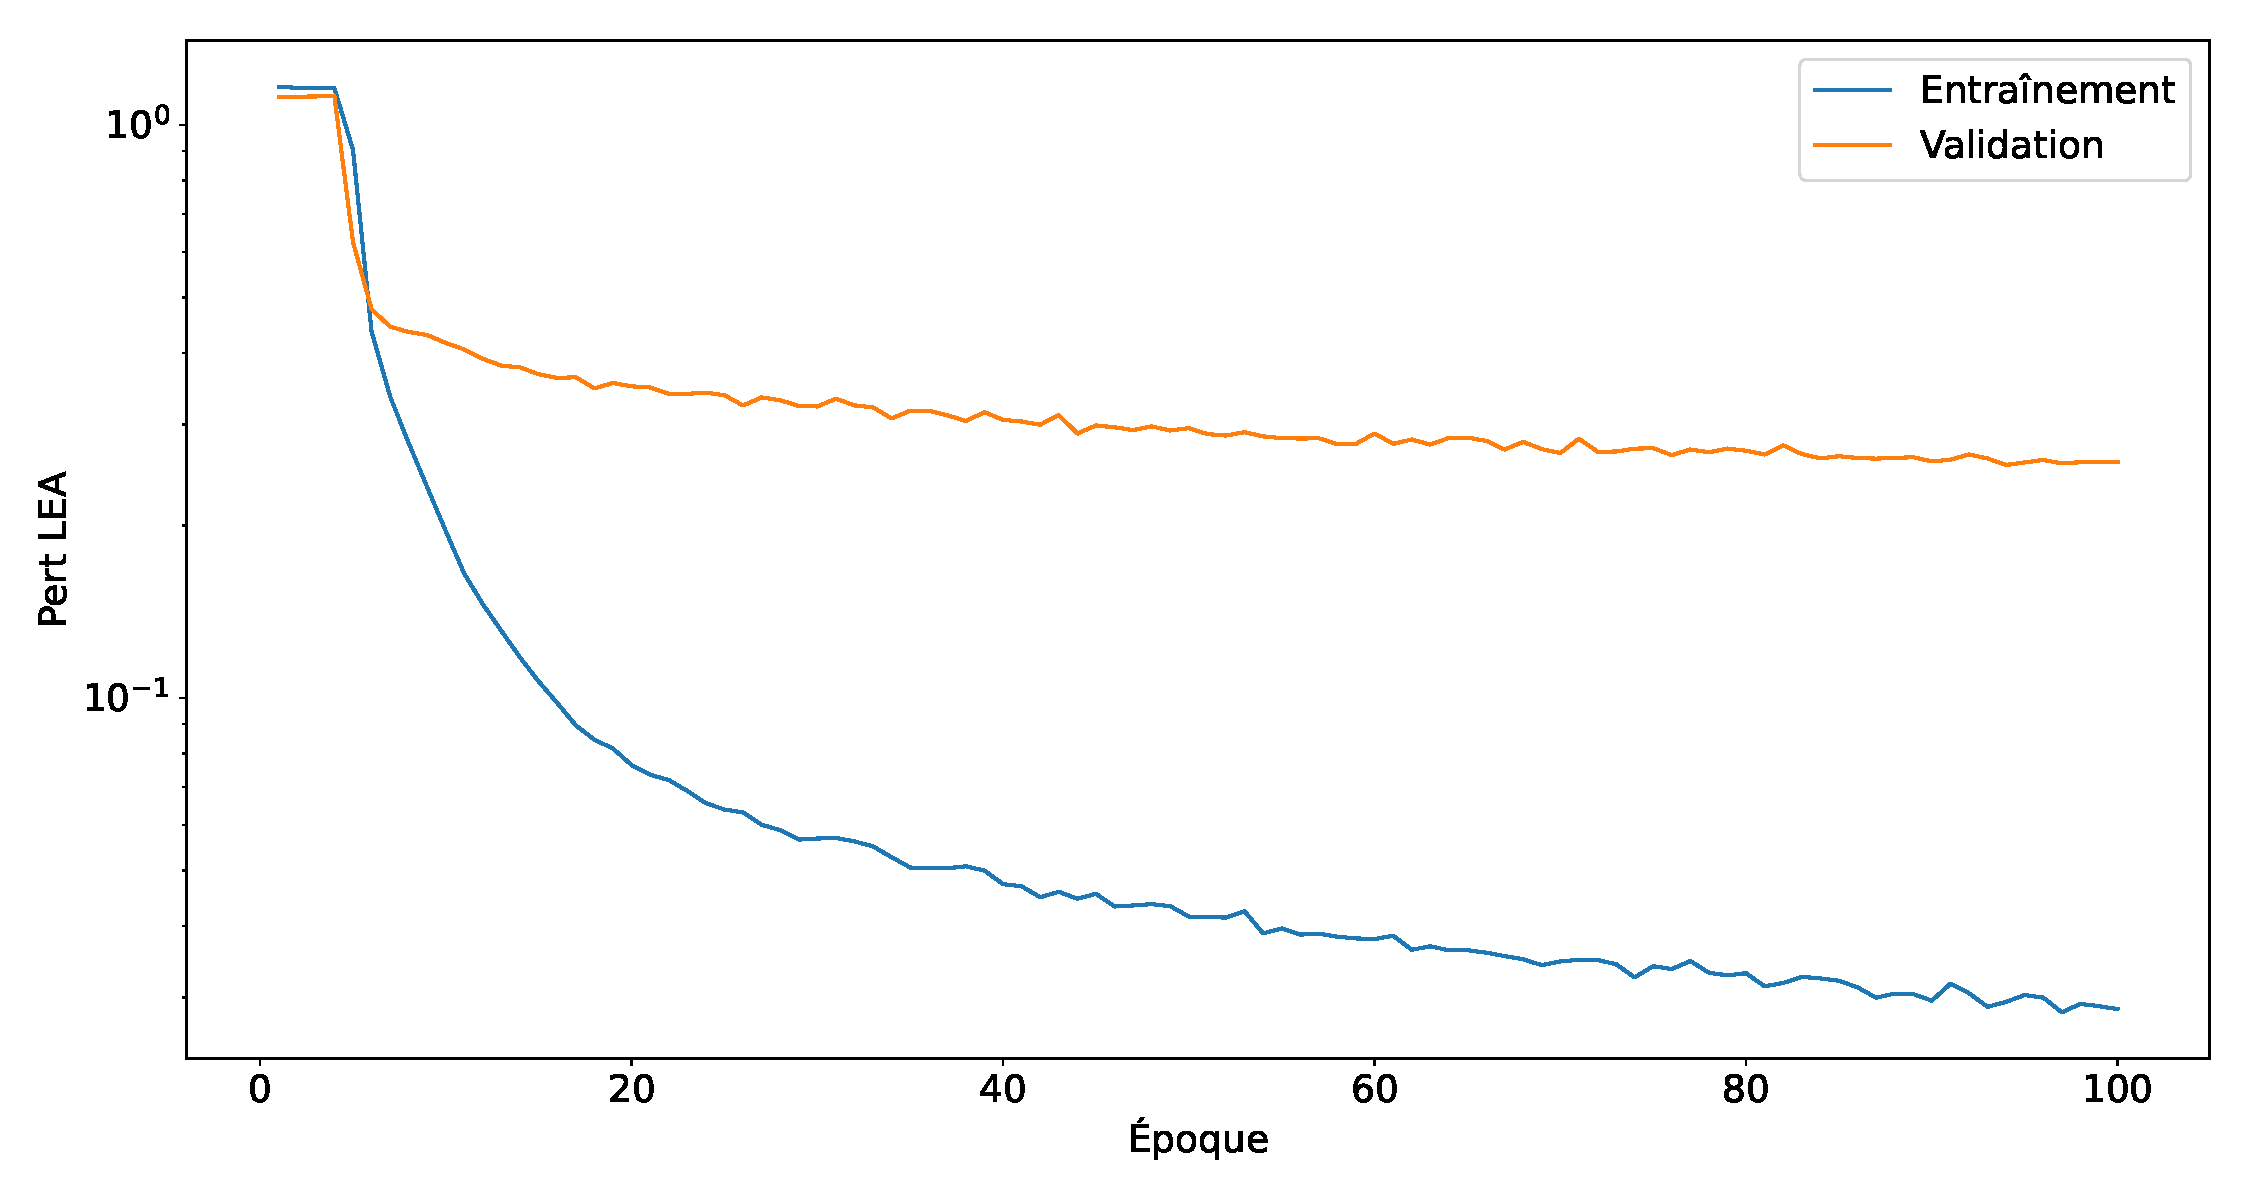
\includegraphics[width=1\linewidth]{images/learning_curves_v3.pdf}
    \caption{Courbes d'entraînement et de validation pour le troisième réseau. On entraîne sur $100$ époques.}
    \label{fig:learning_curves_v3}
\end{figure}
\section{Quatrième réseau}
Le quatrième réseau est le même que le troisième, mais où on a augmenter le taux d'apprentissage à $10^{-3}$. On utilise les mêmes données que le précédent réseau, avec Adam et des mini lots de taille $8$. Augmenter le taux d'apprentissage pourrait accélérer l'entraînement et empêcher le réseau de tomber des extremums qui ne sont pas optimaux, donc potentiellement améliorer la validation. La figure \ref{fig:learning_curves_v4} montre les courbes d'apprentissage du réseau quatre. On note une amélioration non négligeable de la performance en validation avec une perte variant autour de $0.1$, ce qui laisse croire qu'augmenter le taux d'apprentissage permet de meilleurs résultats. On note toutefois d'assez importantes variations de la perte d'une époque à l'autre. Ces variations peuvent être causée par un taux d'apprentissage un peu trop élevé. Avoir un taux entre $10^{-4}$ et $10^{-3}$ pourrait s'avérer intéressant.
\begin{figure}[h!!]
    \centering
    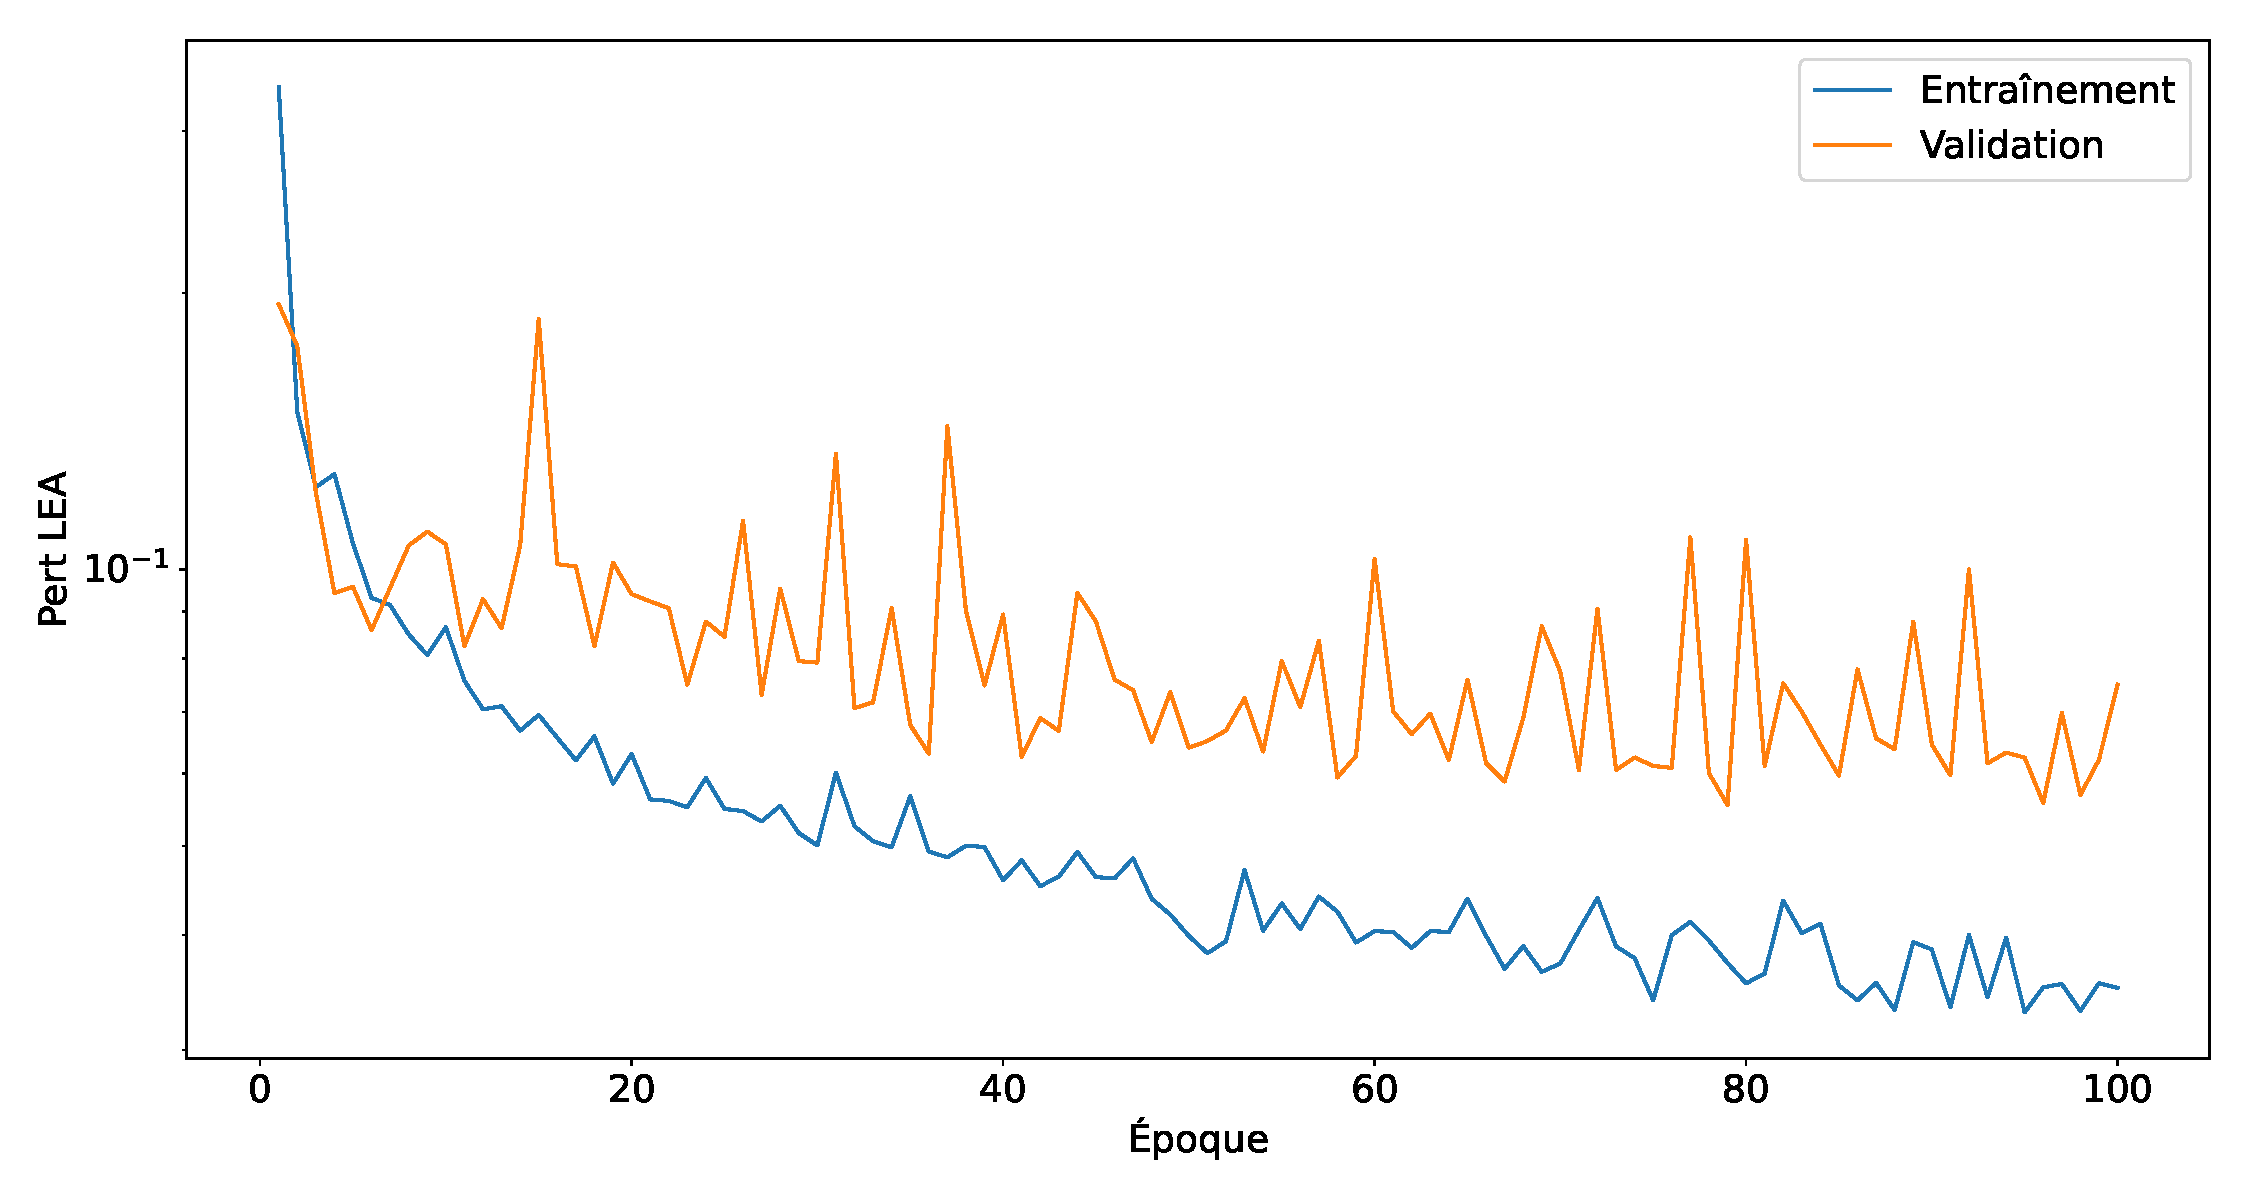
\includegraphics[width=1\linewidth]{images/learning_curves_v4.pdf}
    \caption{Courbes d'entraînement et de validation pour le quatrième réseau. On entraîne sur $100$ époques.}
    \label{fig:learning_curves_v4}
\end{figure}
\newpage
\section{Cinquième réseau}
Le cinquième et dernier réseau présenté dans ce chapitre est le même que le précédent, mais où on réduit de moité le taux d'apprentissage, donnant $5\times 10^{-4}$, soit un entre deux pour le troisième et le quatrième réseau. La figure \ref{fig:learning_curves_v5} montre ses courbes d'apprentissage. On remarque une performance en validation meilleure que les quatre autres réseaux présentés, avec une perte généralement sous la barre de $0.1$. On remarque encore quelques fortes variations, donc il resterait de l'optimisation à faire pour adoucir la courbe de validation.
\begin{figure}[h!!]
    \centering
    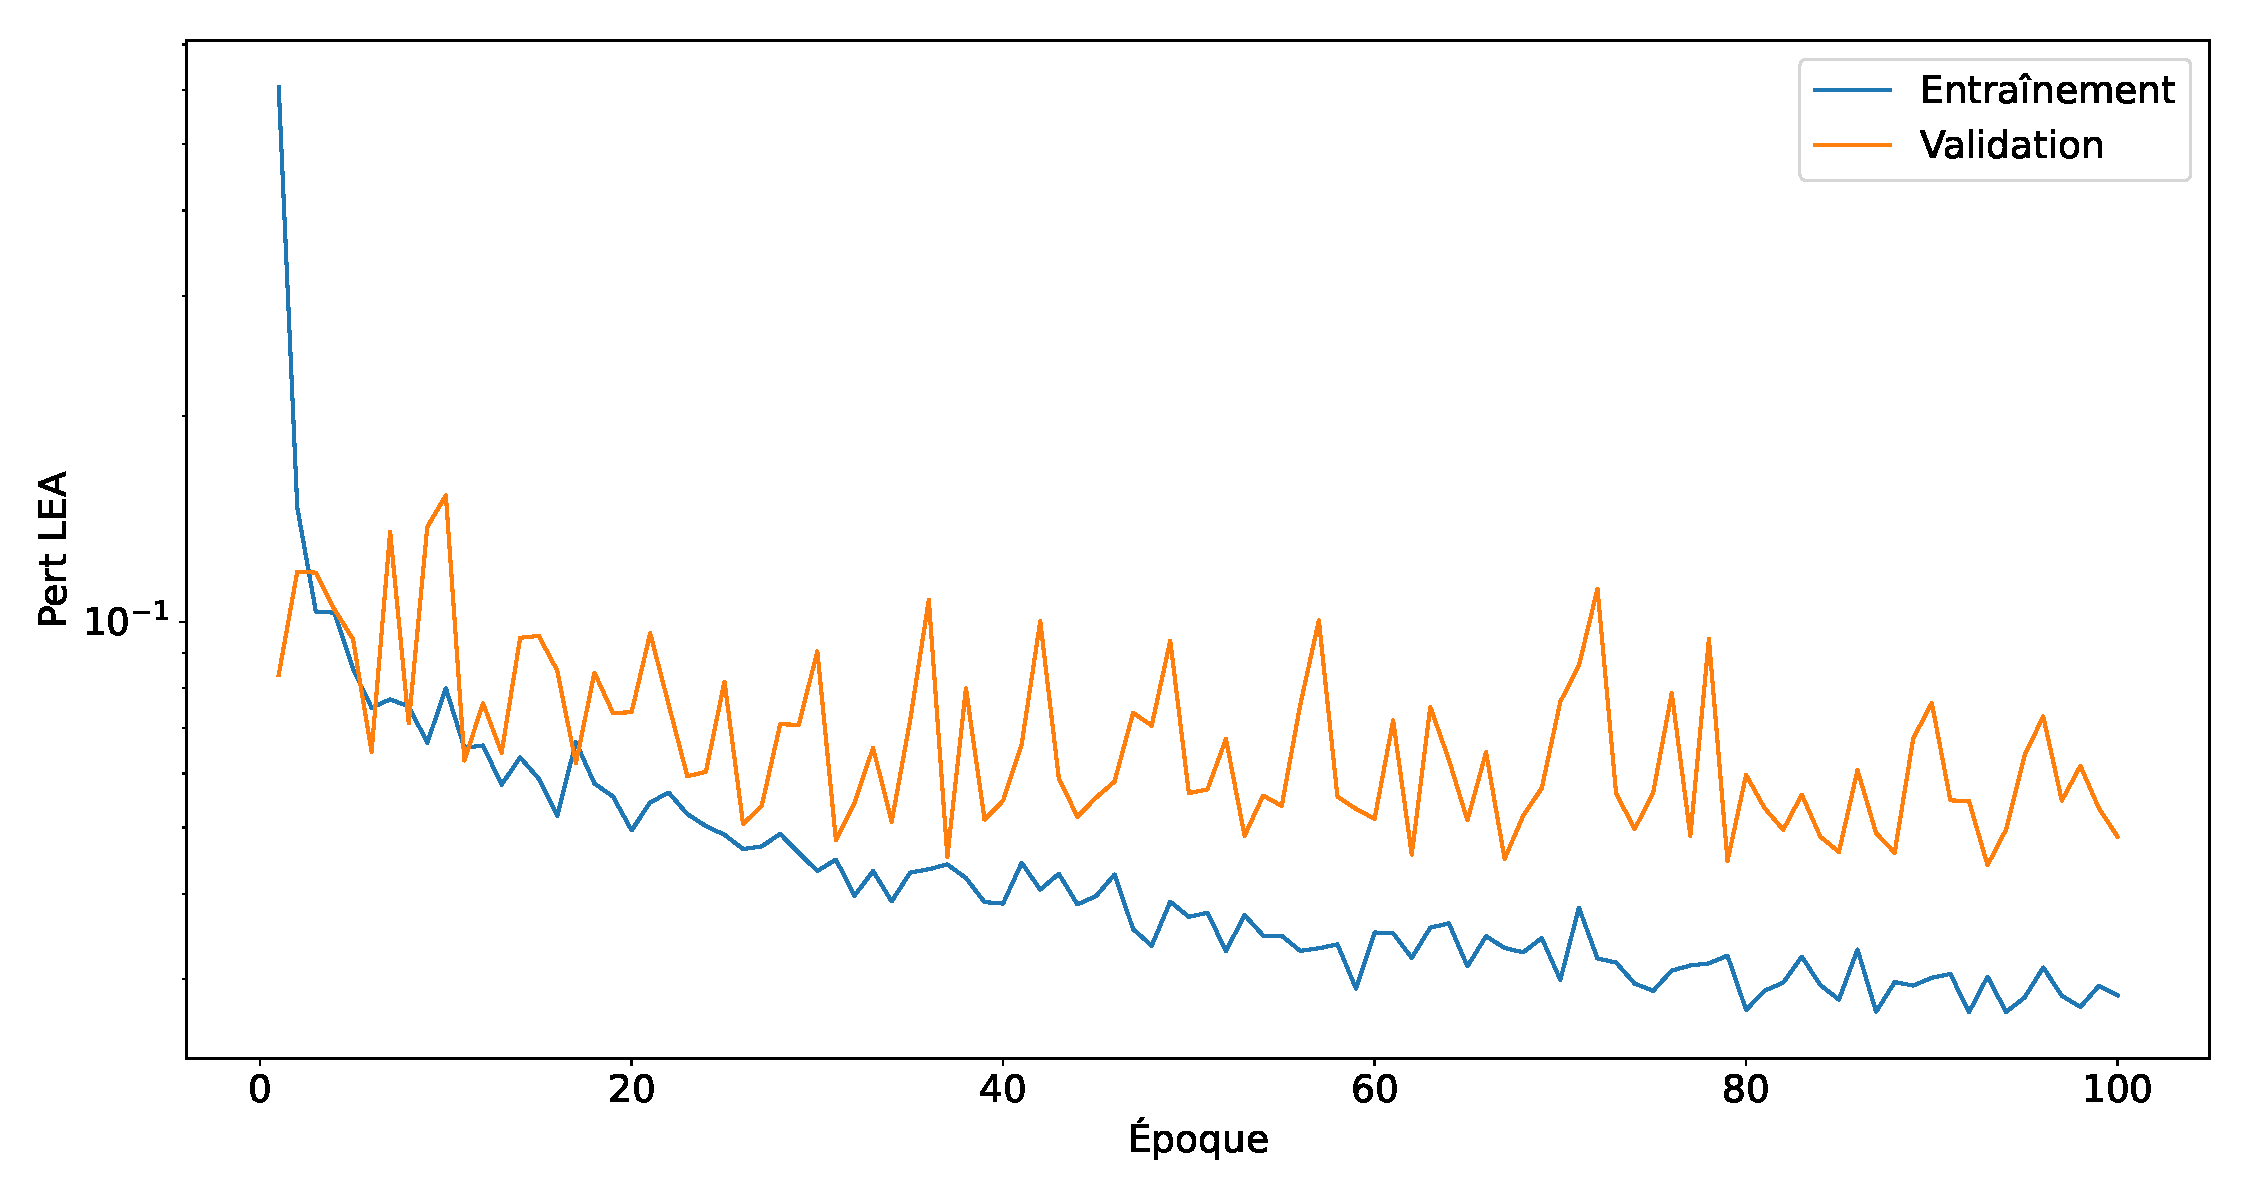
\includegraphics[width=1\linewidth]{images/learning_curves_v5.pdf}
    \caption{Courbes d'entraînement et de validation pour le cinquième réseau. On entraîne sur $100$ époques.}
    \label{fig:learning_curves_v5}
\end{figure}
\newpage
\section{Autres métriques d'analyse}
La perte LEA est intéressante pour avoir une vue globale. Par contre, elle ne permet pas vraiment d'évaluer la justesse du réseau dans sa pleine complexité. On a vu au chapitre précédent que selon le ratio $T/\tau_c$, l'apprentissage se fait plus ou moins difficilement. Il faut donc s'intéresser à la précision en fonction du temps caractéristique ciblé.
\subsection{Premier réseau}
Pour le premier réseau, la figure \ref{fig:LAE_vs_tau_c_v1} montre la log erreur absolue en fonction du $\tau_c$ cible.
\begin{figure}[h!!]
    \centering
    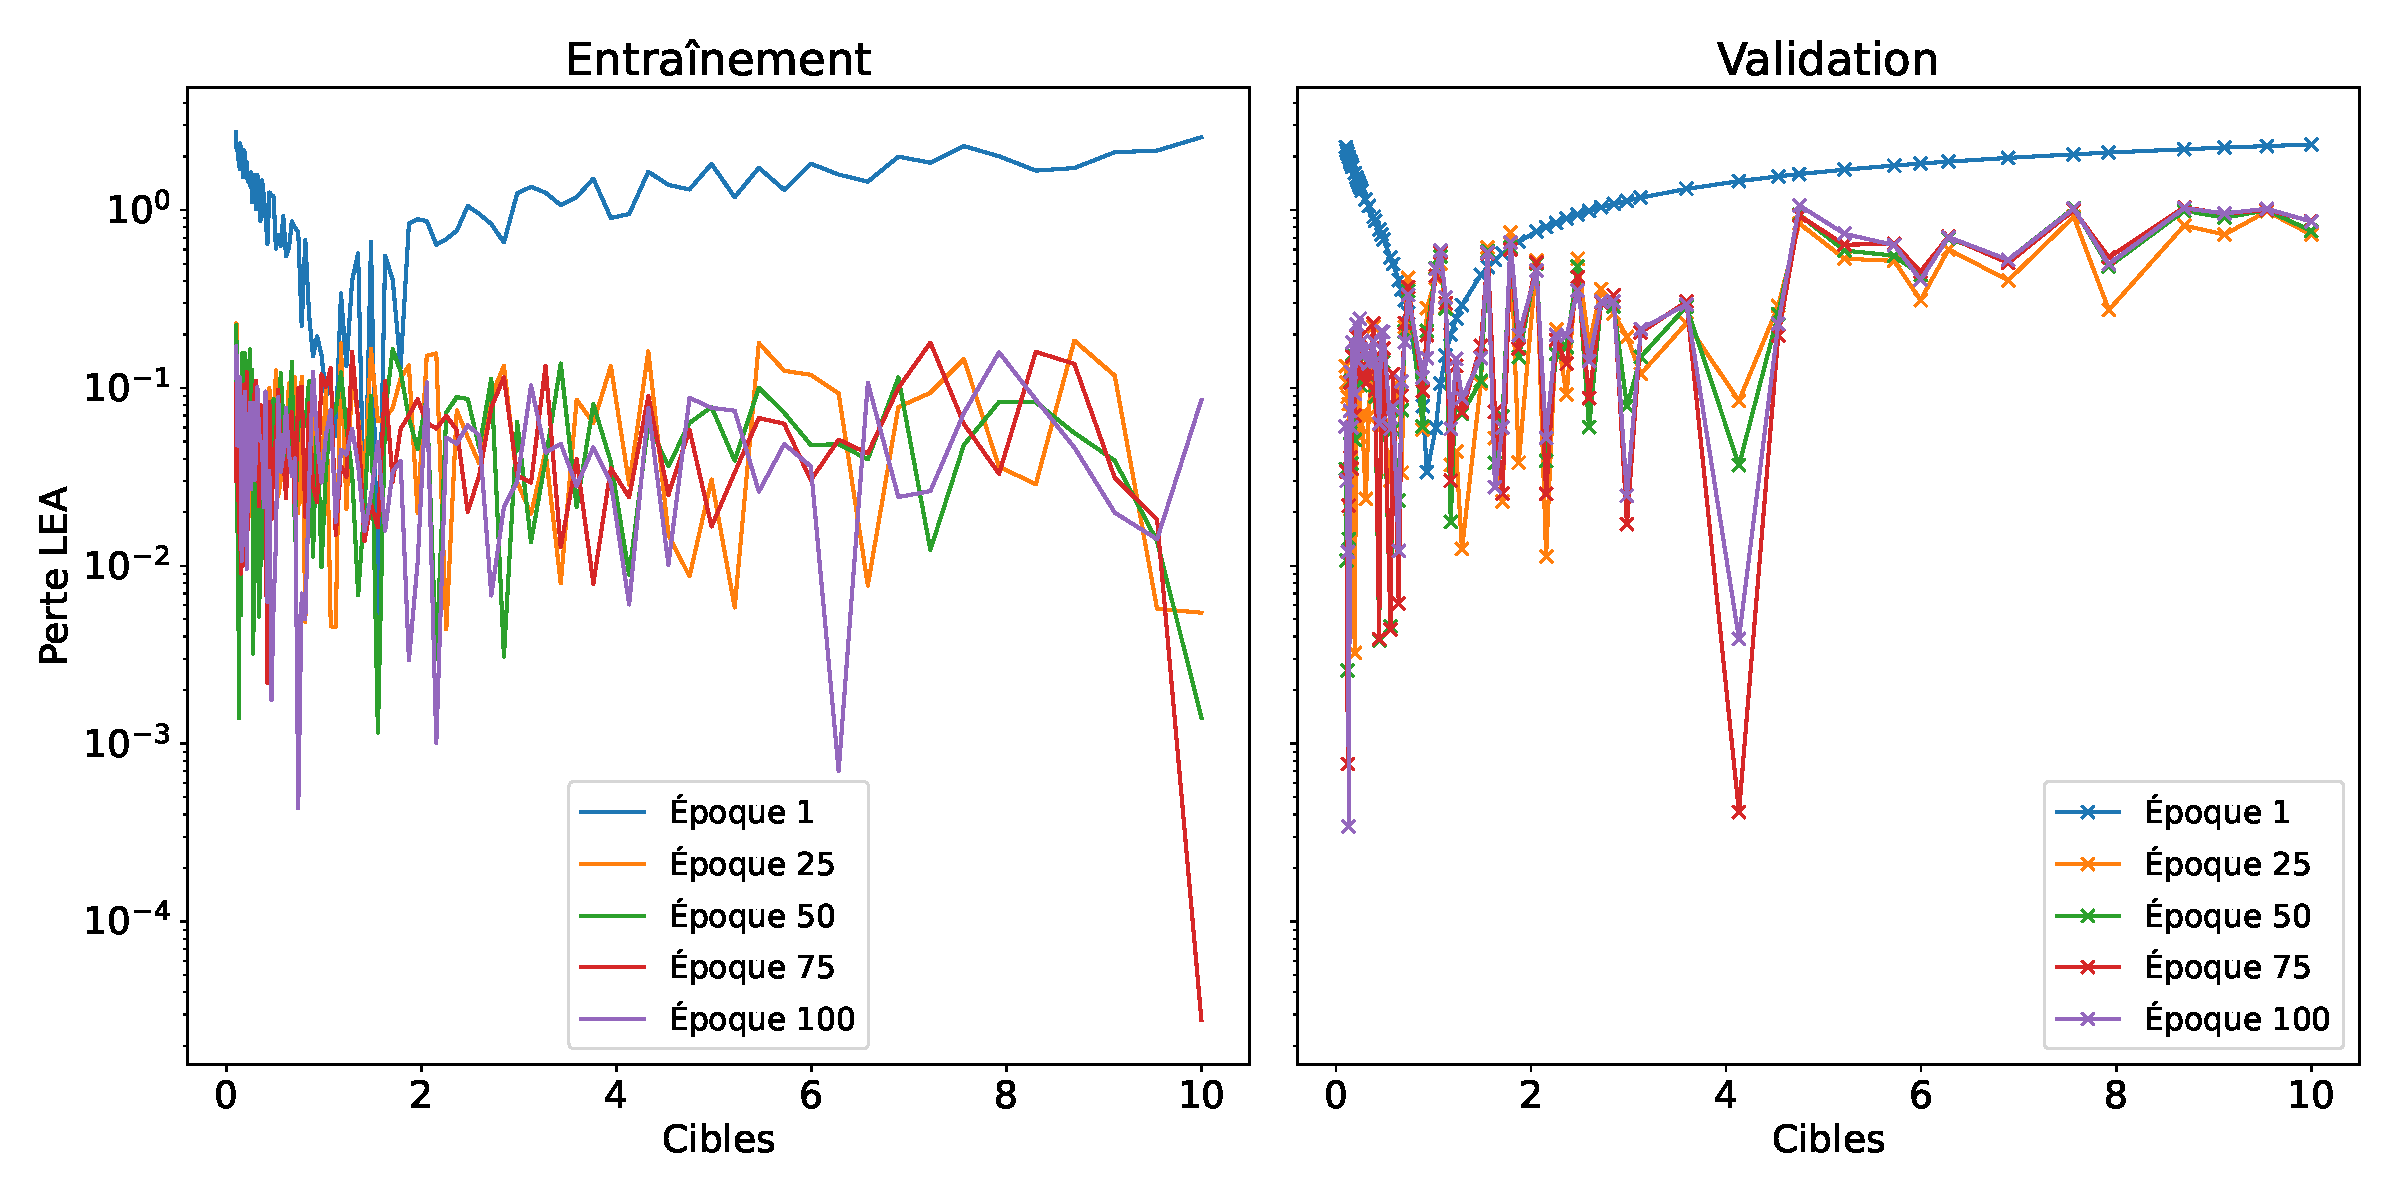
\includegraphics[width=\linewidth]{images/LAEVsTargs_v1.pdf}
    \caption{Perte log erreur absolue du premier réseau en fonction des cibles pour l'entraînement et la validation. On affiche quelques époques par graphique.}
    \label{fig:LAE_vs_tau_c_v1}
\end{figure}
On remarque que l'entraînement se fait bien, avec une perte généralement entre $0.1$ et $0.01$ pour la plupart des époques affichées. Ce constat n'est pas nouveau, on savait déjà que le réseau avait un apprentissage en entraînement très bon. Pour la validation, ce n'est pas pareil. On remarque un perte plus élevée et qui semble augmenter avec la grandeur des cibles. Ce constat est confirmé à la figure \ref{fig:predsVsTargs_v1} qui montre $\hat{\tau}_c$ en fonction de $\tau_c$. La légende contient, en plus de l'époque associée à la couleur de la courbe, le score $R^2$, soit la qualité de la régression linéaire entre les prédictions et les cibles. On remarque, en validation, que plus la valeur de la cible augmente, plus le réseau devient imprécis. On peut aussi se concenter sur la figure \ref{fig:predsVsTargs_v1_log} qui montre aussi $\hat{\tau}_c$ en fonction de $\tau_c$, mais en échelle logarithmique, ce qui peut être plus représentatif de l'apprentissage, car c'est sur cet échelle qu'on calcule la perte après tout. L'avantage de l'échelle logarithmique est principalement de mieux voir le comportement des cibles de petites valeurs. On y remarque une bonne précision, d'où les coefficients de détermination $R^2$ plus élevés, mais elle diminue avec l'amplitude de la cible.
\newpage
\begin{figure}[h!!]
    \centering
    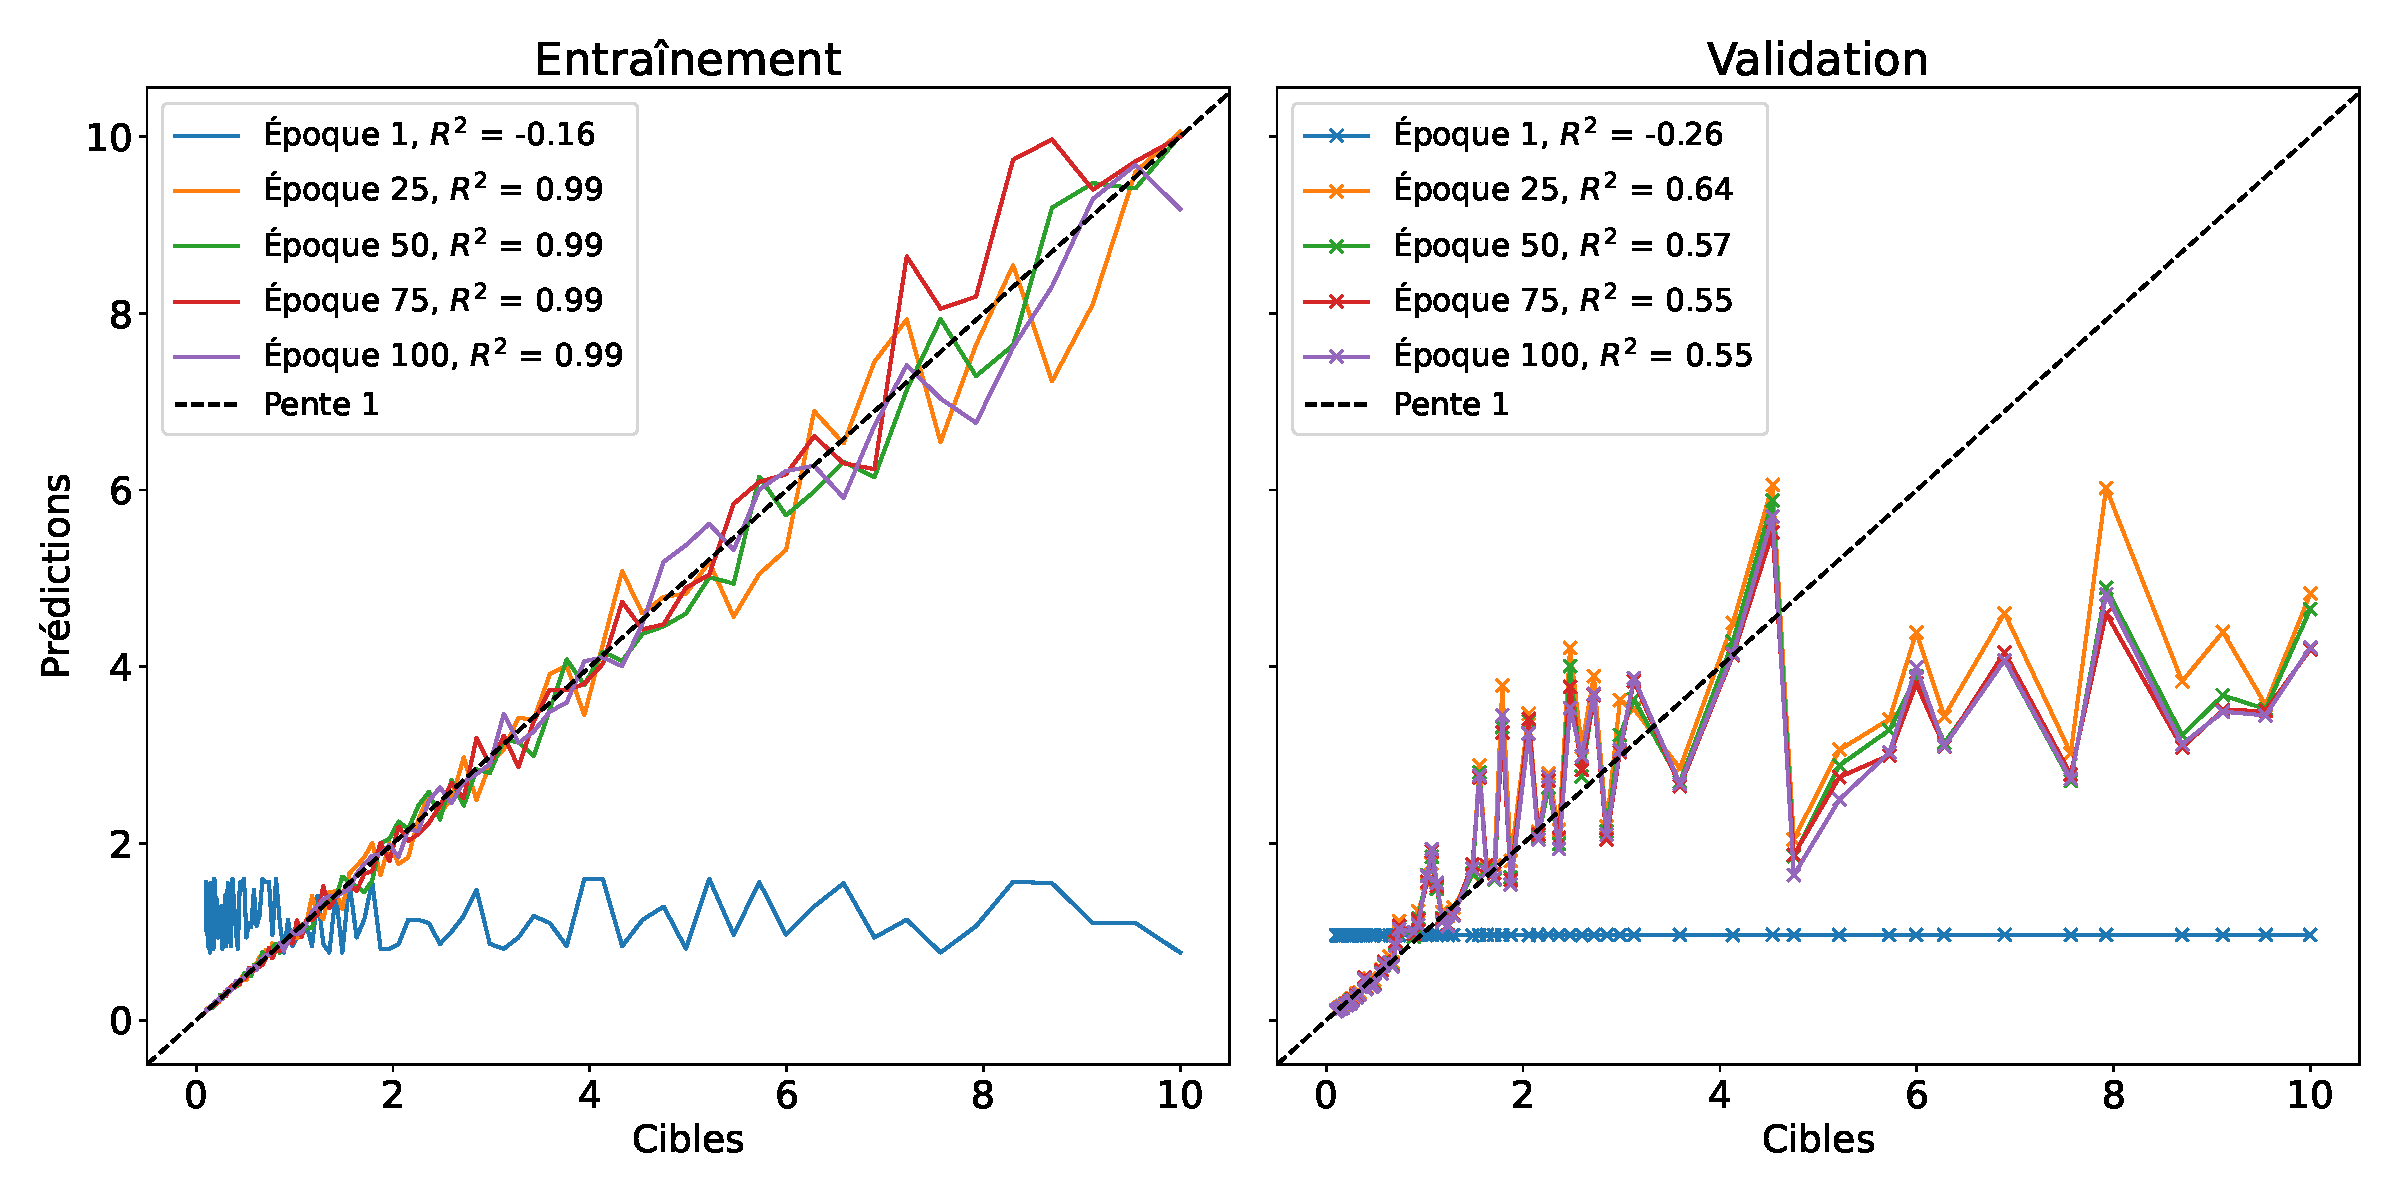
\includegraphics[width=\linewidth]{images/predsVsTargs_v1.pdf}
    \caption{Prédictions en fonction des cibles du le premier réseau pour l'entraînement et la validation. On affiche quelques époques par graphique.}
    \label{fig:predsVsTargs_v1}
\end{figure}
\begin{figure}[h!!]
    \centering
    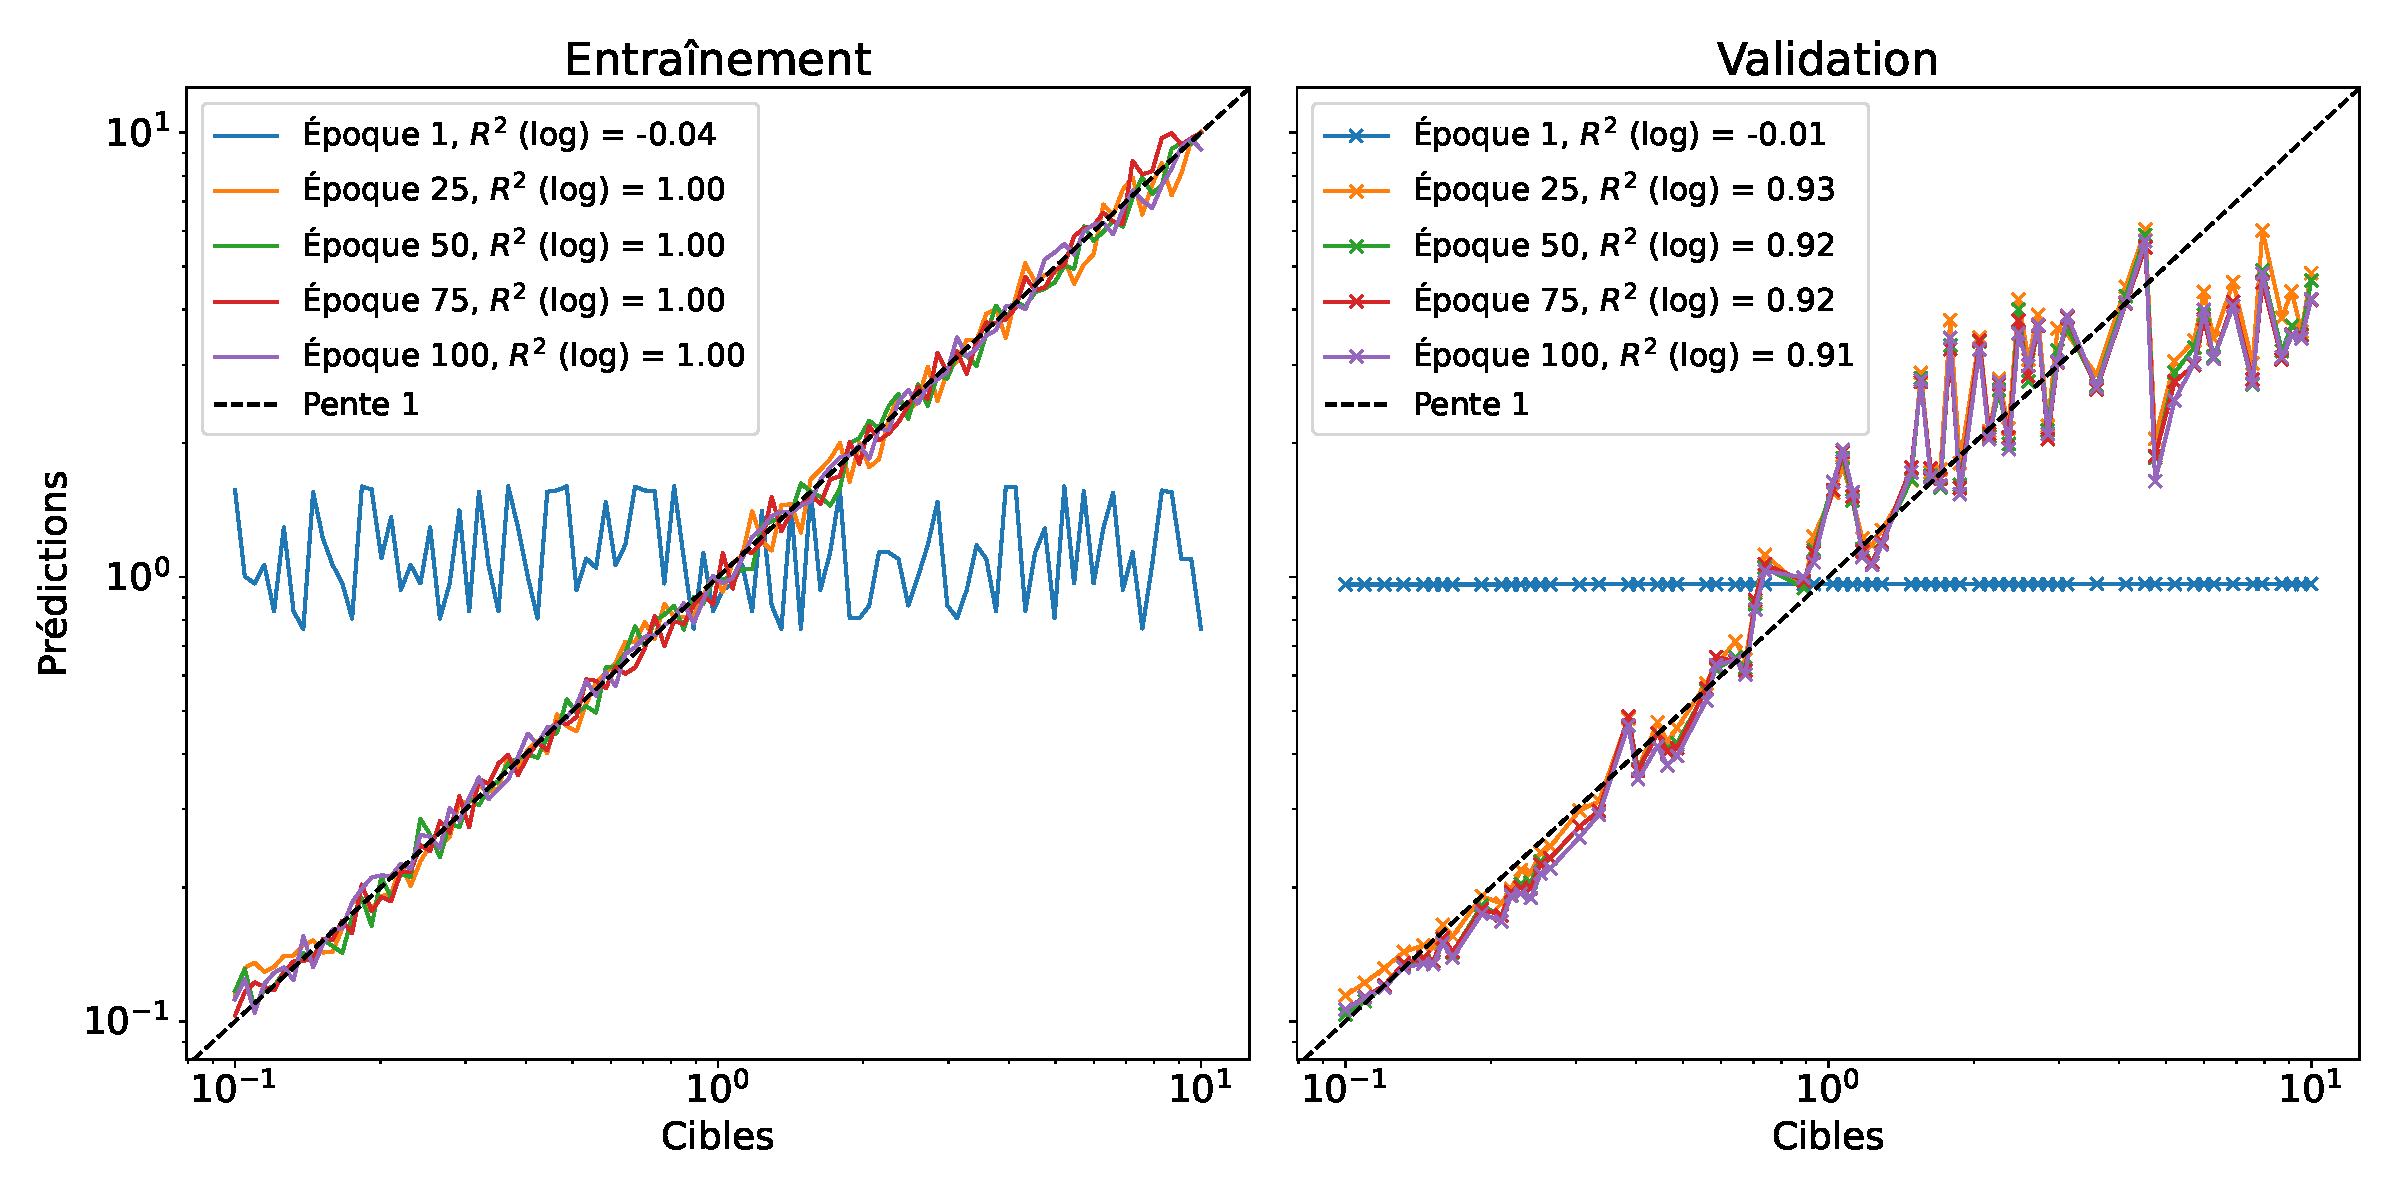
\includegraphics[width=\linewidth]{images/predsVsTargs_v1_log.pdf}
    \caption{Log-prédictions en fonction des log-cibles du le premier réseau pour l'entraînement et la validation. On affiche quelques époques par graphique.}
    \label{fig:predsVsTargs_v1_log}
\end{figure}
\newpage
\subsection{Deuxième réseau}
Pour le second réseau, les mêmes métriques sont évaluées. La figure \ref{fig:LAE_vs_tau_c_v2} montre la perte en fonction de la cible. La principale conclusion des courbes d'entraînement est vérifiée ici, soit qu'un réseau plus petit n'apporte pas, dans ce cas-ci, de dégradation de performances.
\begin{figure}[h!!]
    \centering
    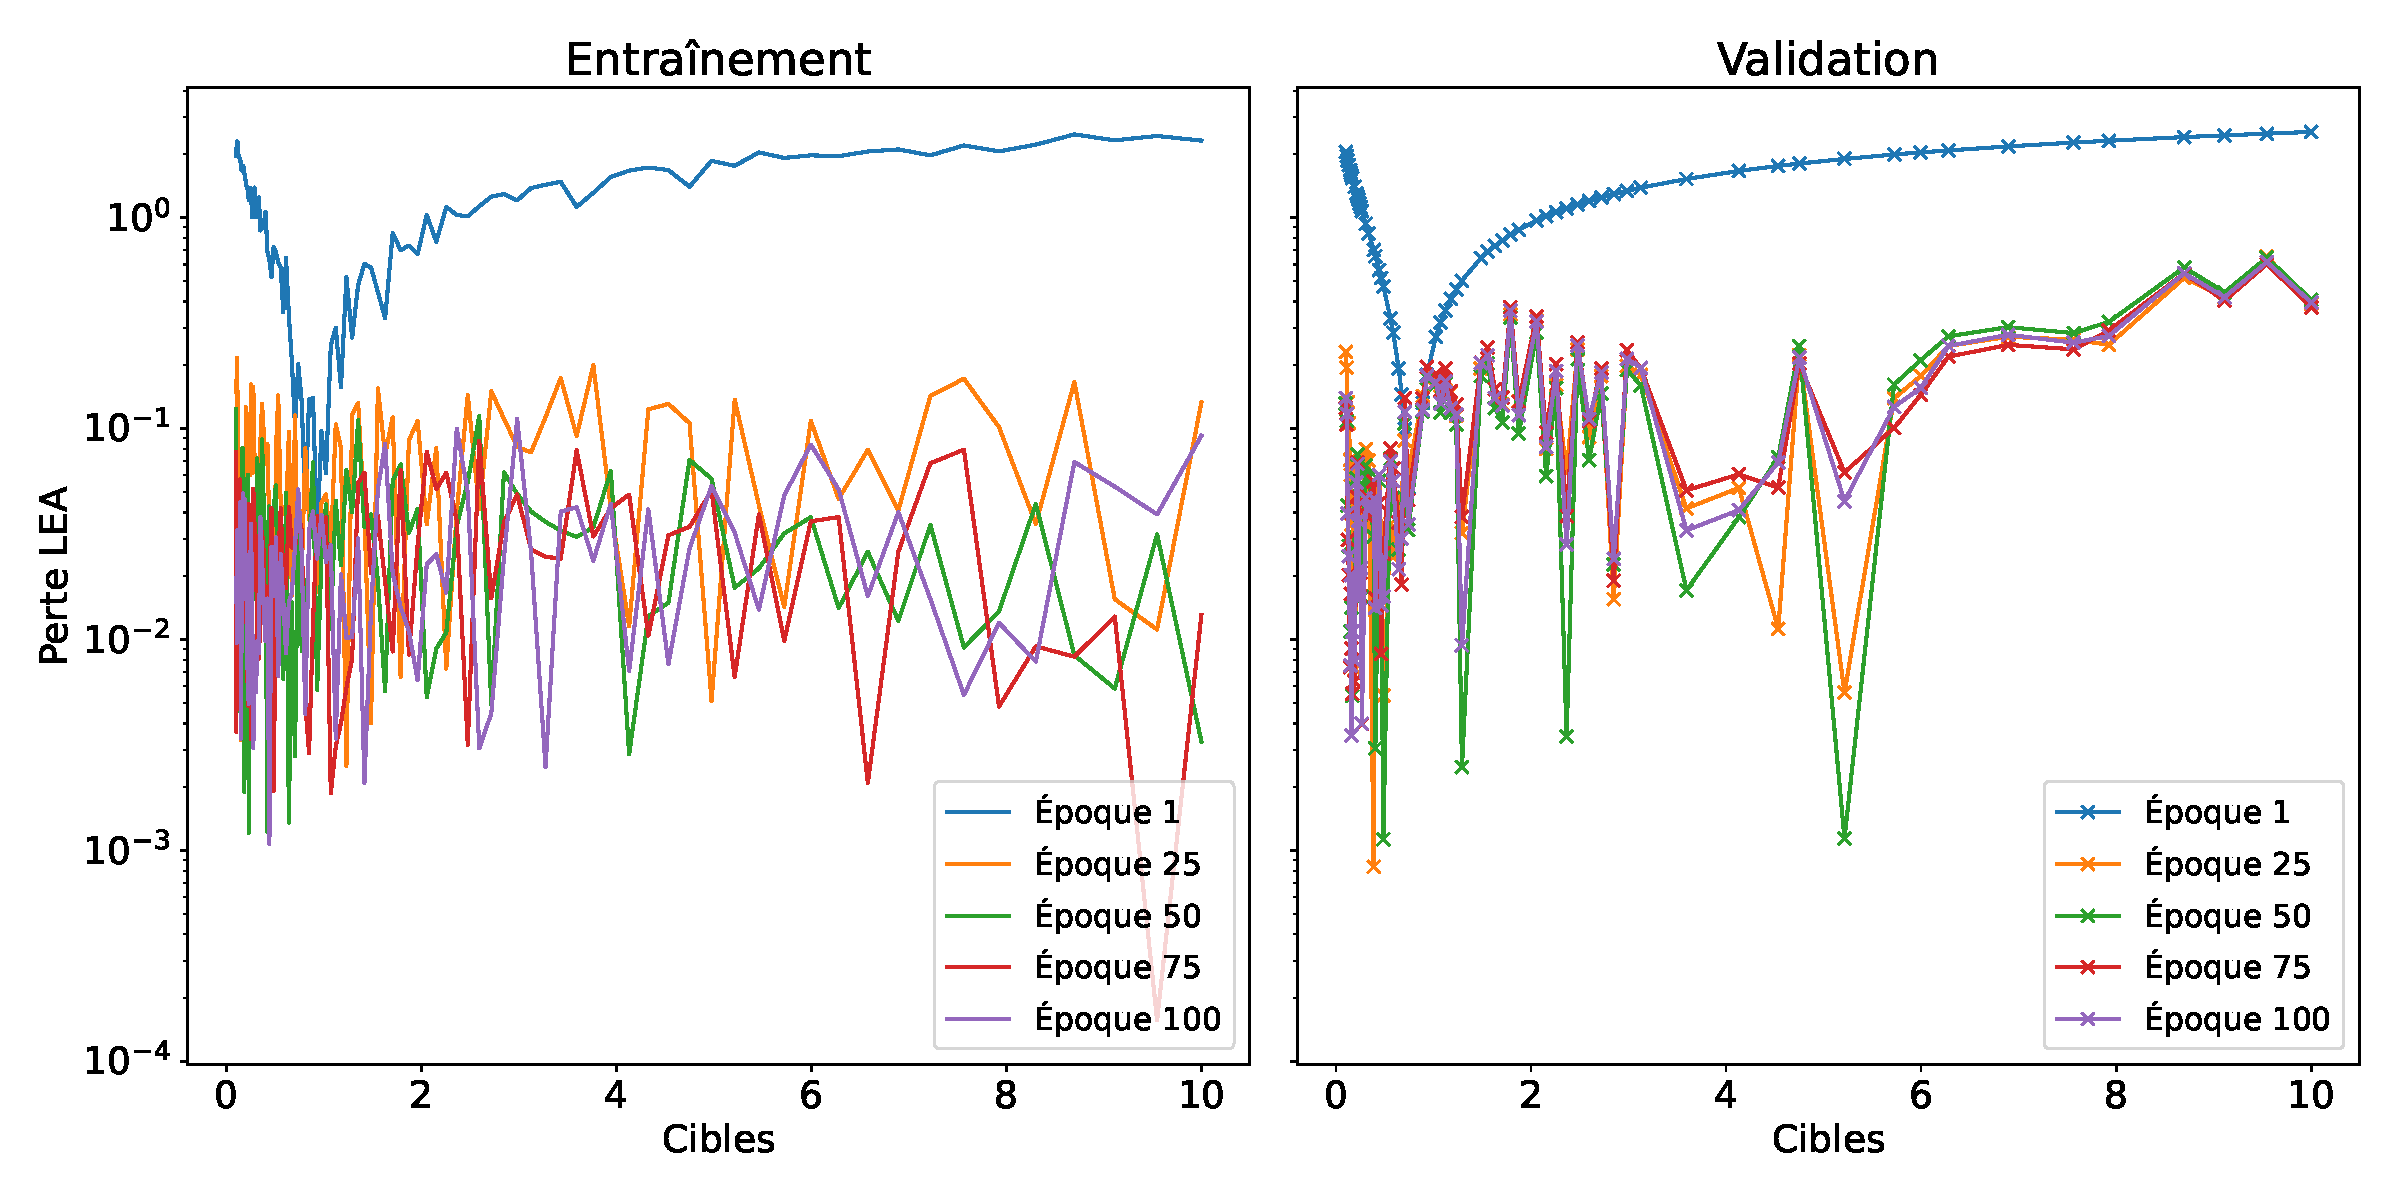
\includegraphics[width=\linewidth]{images/LAEVsTargs_v2.pdf}
    \caption{Perte log erreur absolue du deuxième réseau en fonction des cibles pour l'entraînement et la validation. On affiche quelques époques par graphique.}
    \label{fig:LAE_vs_tau_c_v2}
\end{figure}
On y voit aussi une certaine perte de performance avec la montée en grandeur de la cible, comme pour le premier réseau. La figure \ref{fig:predsVsTargs_v2}, et la figure \ref{fig:predsVsTargs_v2_log} pour l'échelle logarithmique, donnent la même conclusion sur la performance.
\begin{figure}[h!!]
    \centering
    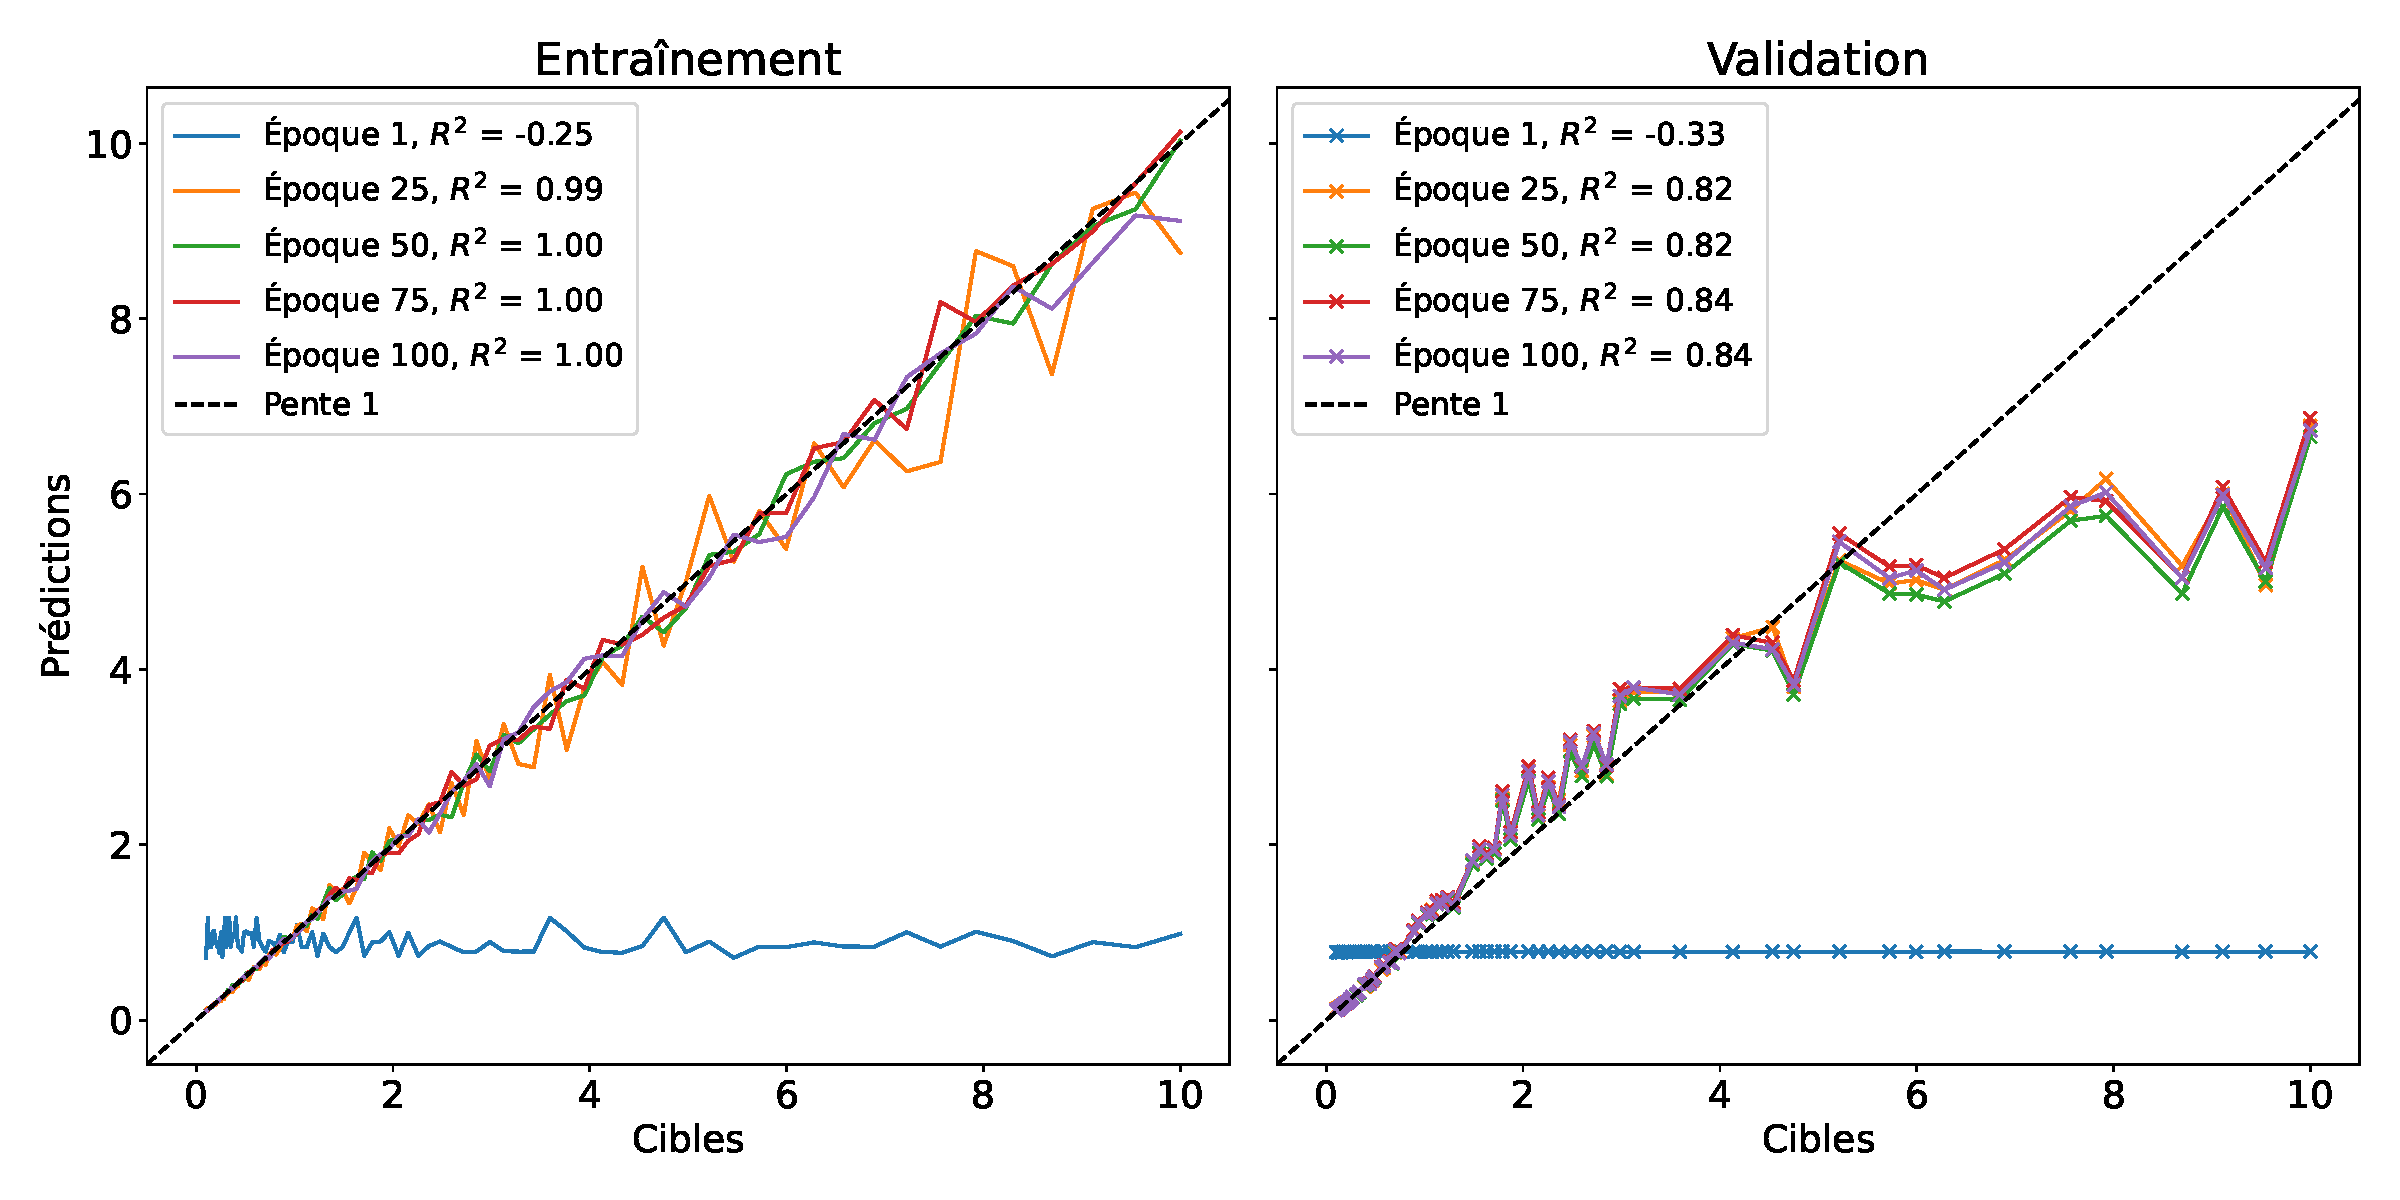
\includegraphics[width=\linewidth]{images/predsVsTargs_v2.pdf}
    \caption{Prédictions en fonction des cibles du le deuxième réseau pour l'entraînement et la validation. On affiche quelques époques par graphique.}
    \label{fig:predsVsTargs_v2}
\end{figure}
On y note aussi, dans les deux cas, des coefficients de détermination plus élevés que pour le premier réseau. Il est intéressant de constater que ces conclusions ne sont pas évidentes avec les courbes d'entraînement seules, notamment car elles moyennent sur les divers régimes de $\tau_c$. On voit finalement que la linéarité est mieux préservée dans l'espace log pour les hauts temps caractéristique dans ce second cas comparativement au premier cas.
\begin{figure}[h!!]
    \centering
    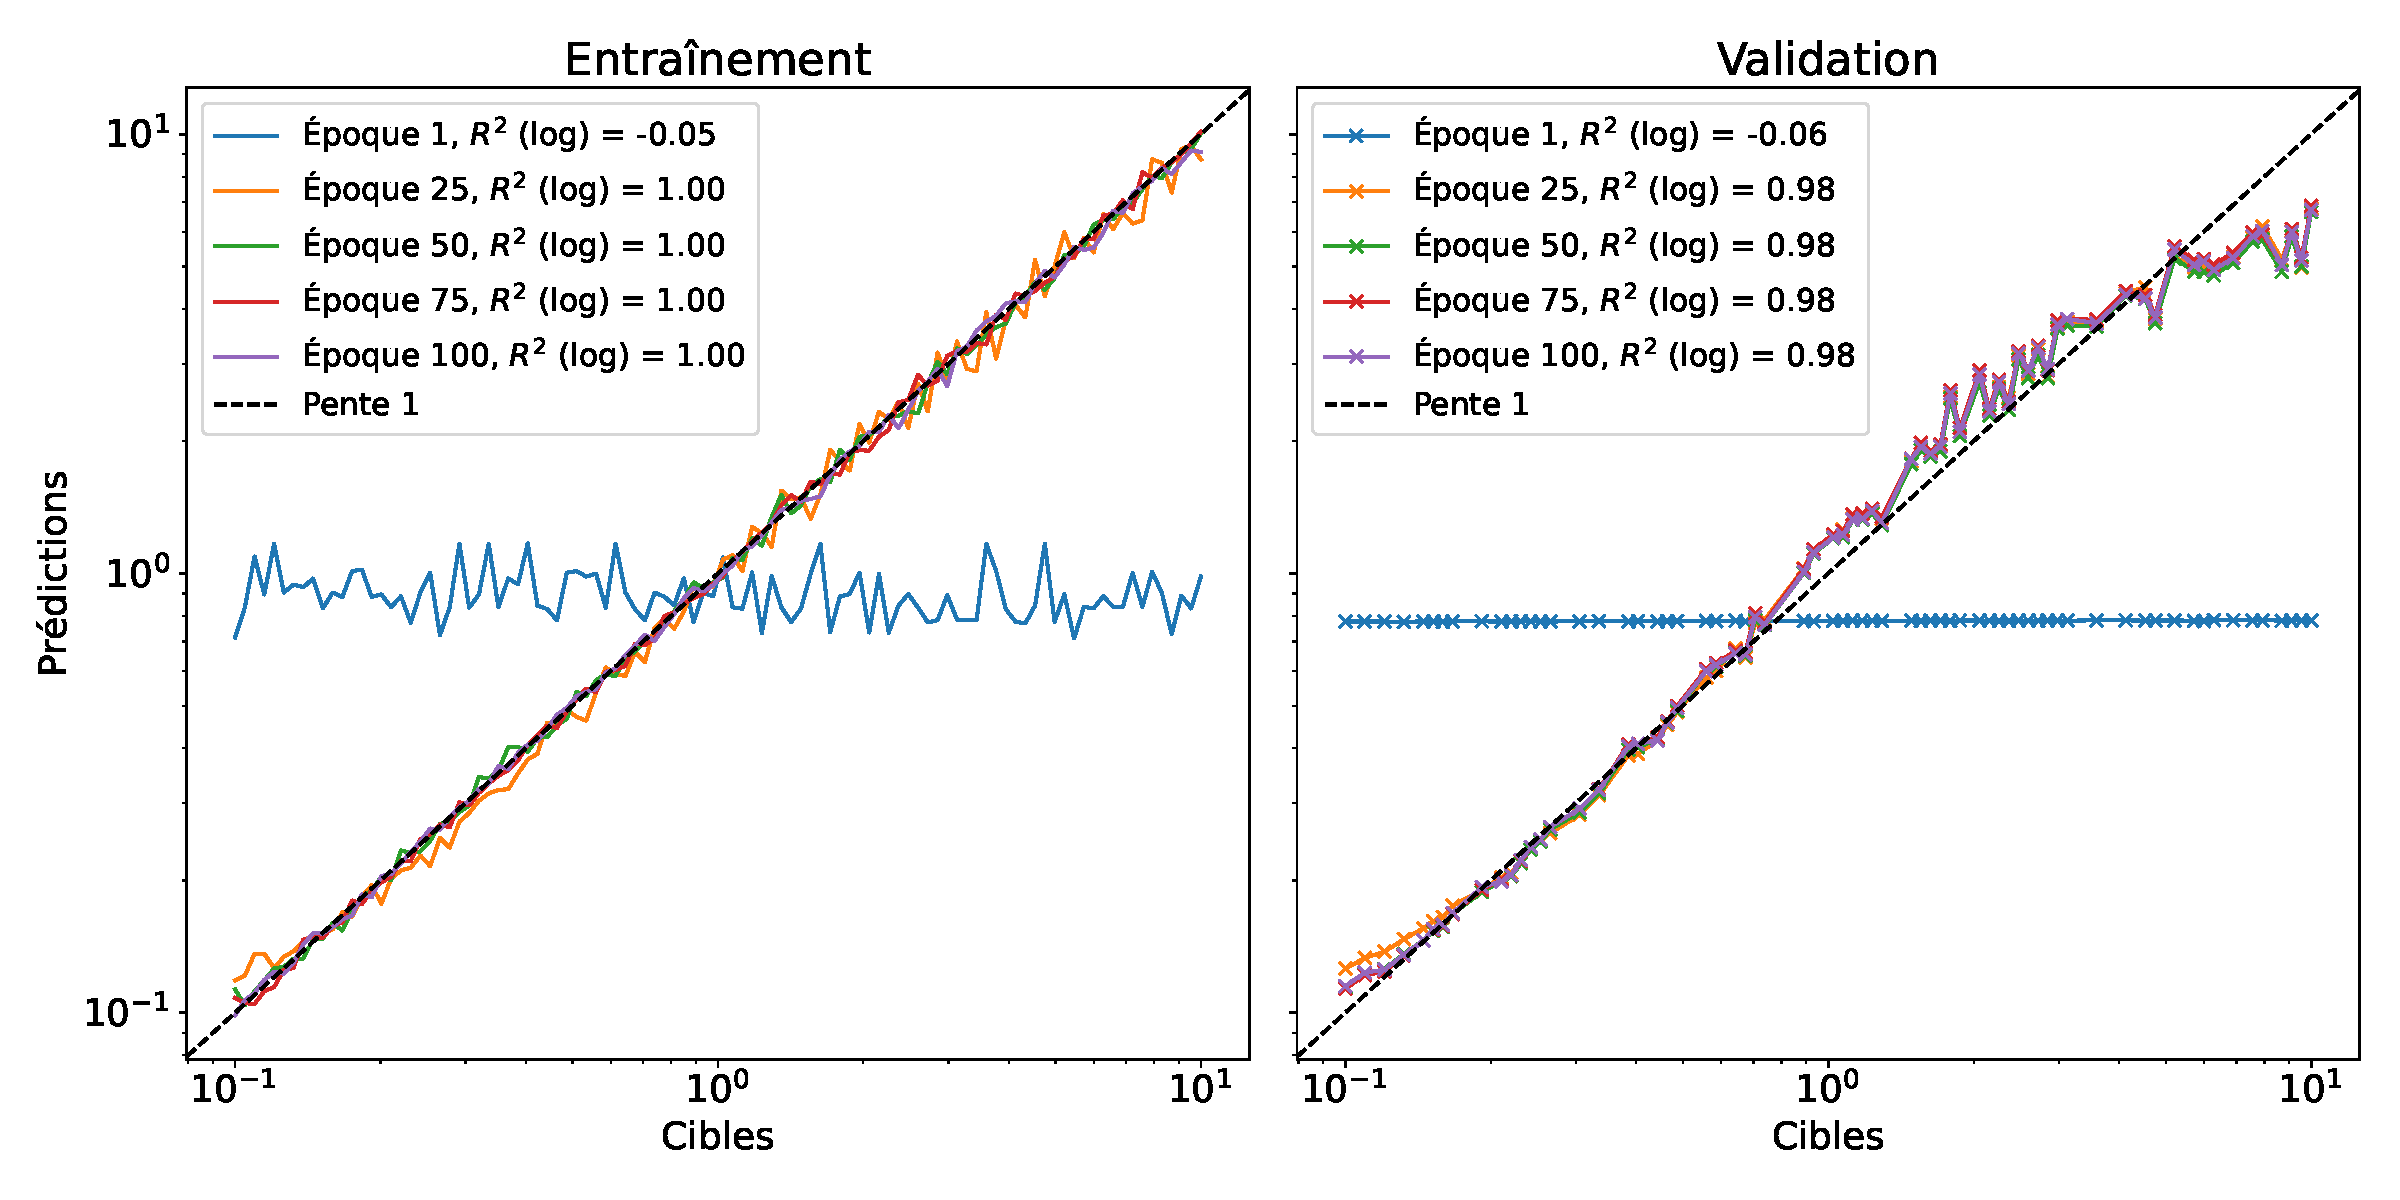
\includegraphics[width=\linewidth]{images/predsVsTargs_v2_log.pdf}
    \caption{Log-prédictions en fonction des log-cibles du le deuxième réseau pour l'entraînement et la validation. On affiche quelques époques par graphique.}
    \label{fig:predsVsTargs_v2_log}
\end{figure}
\newpage
\subsection{Troisième réseau}
Pour le troisième réseau, la perte en fonction des cibles est présentée à la figure \ref{fig:LAE_vs_tau_c_v3}. On y voit qu'en tant que tel, ajouter des données n'est pas nécessairement mieux, car on a des performances proches du précédent réseau. Les figure de $\hat{\tau}_c$ en fonction de $\tau_c$, soit \ref{fig:predsVsTargs_v3} et \ref{fig:predsVsTargs_v3_log} pour l'échelle log, montrent la même conclusion, notamment par les coefficients de détermination.
\begin{figure}[h!!]
    \centering
    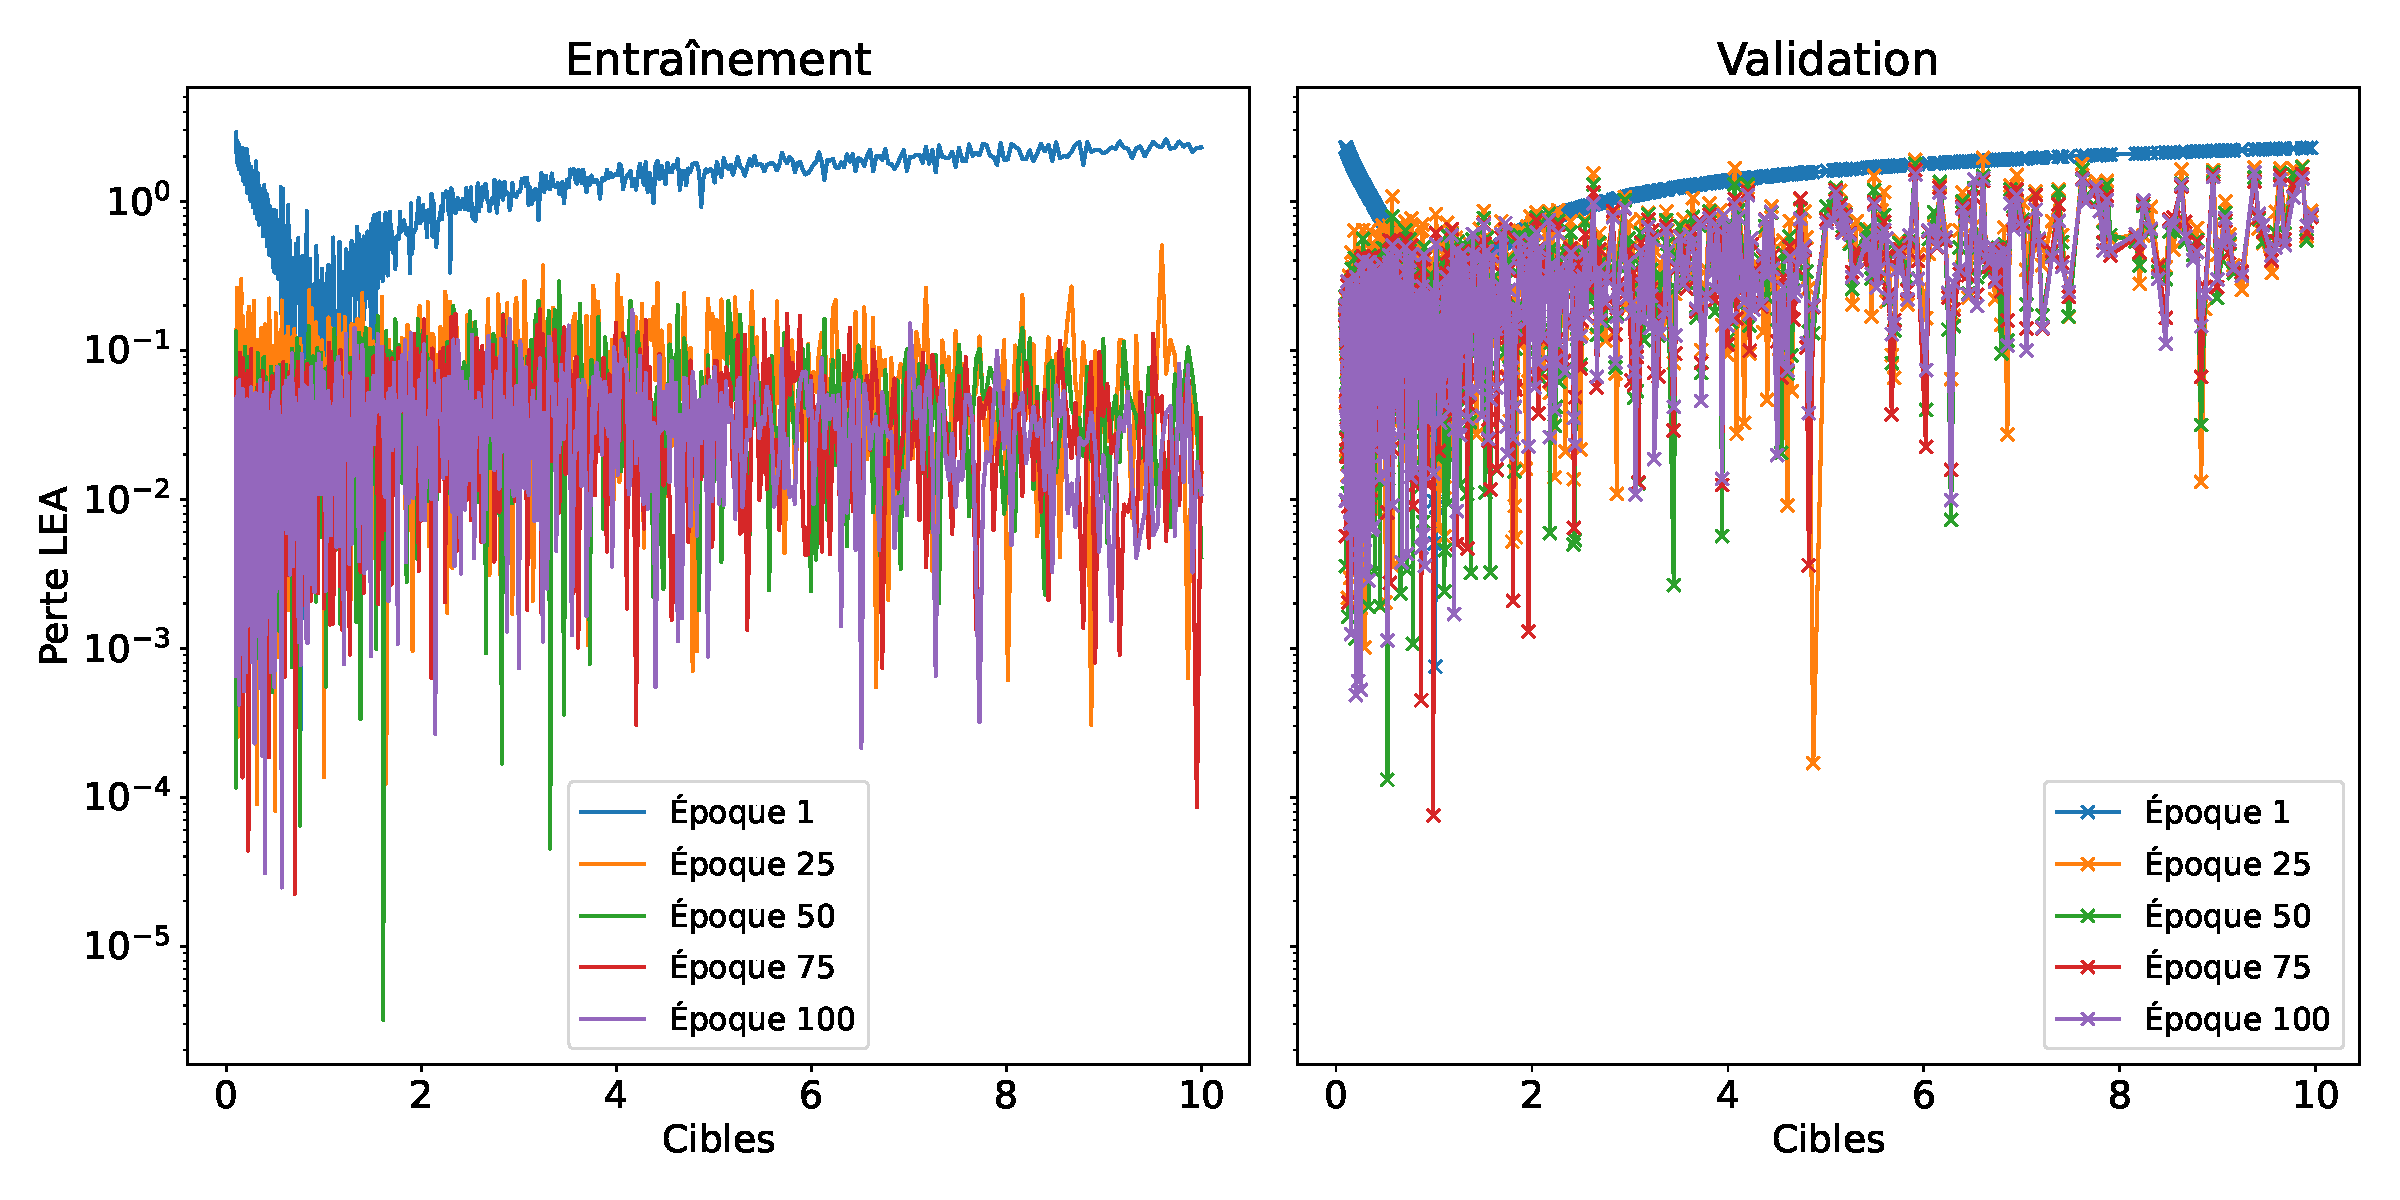
\includegraphics[width=\linewidth]{images/LAEVsTargs_v3.pdf}
    \caption{Perte log erreur absolue du troisième réseau en fonction des cibles pour l'entraînement et la validation. On affiche quelques époques par graphique.}
    \label{fig:LAE_vs_tau_c_v3}
\end{figure}
\begin{figure}[h!!]
    \centering
    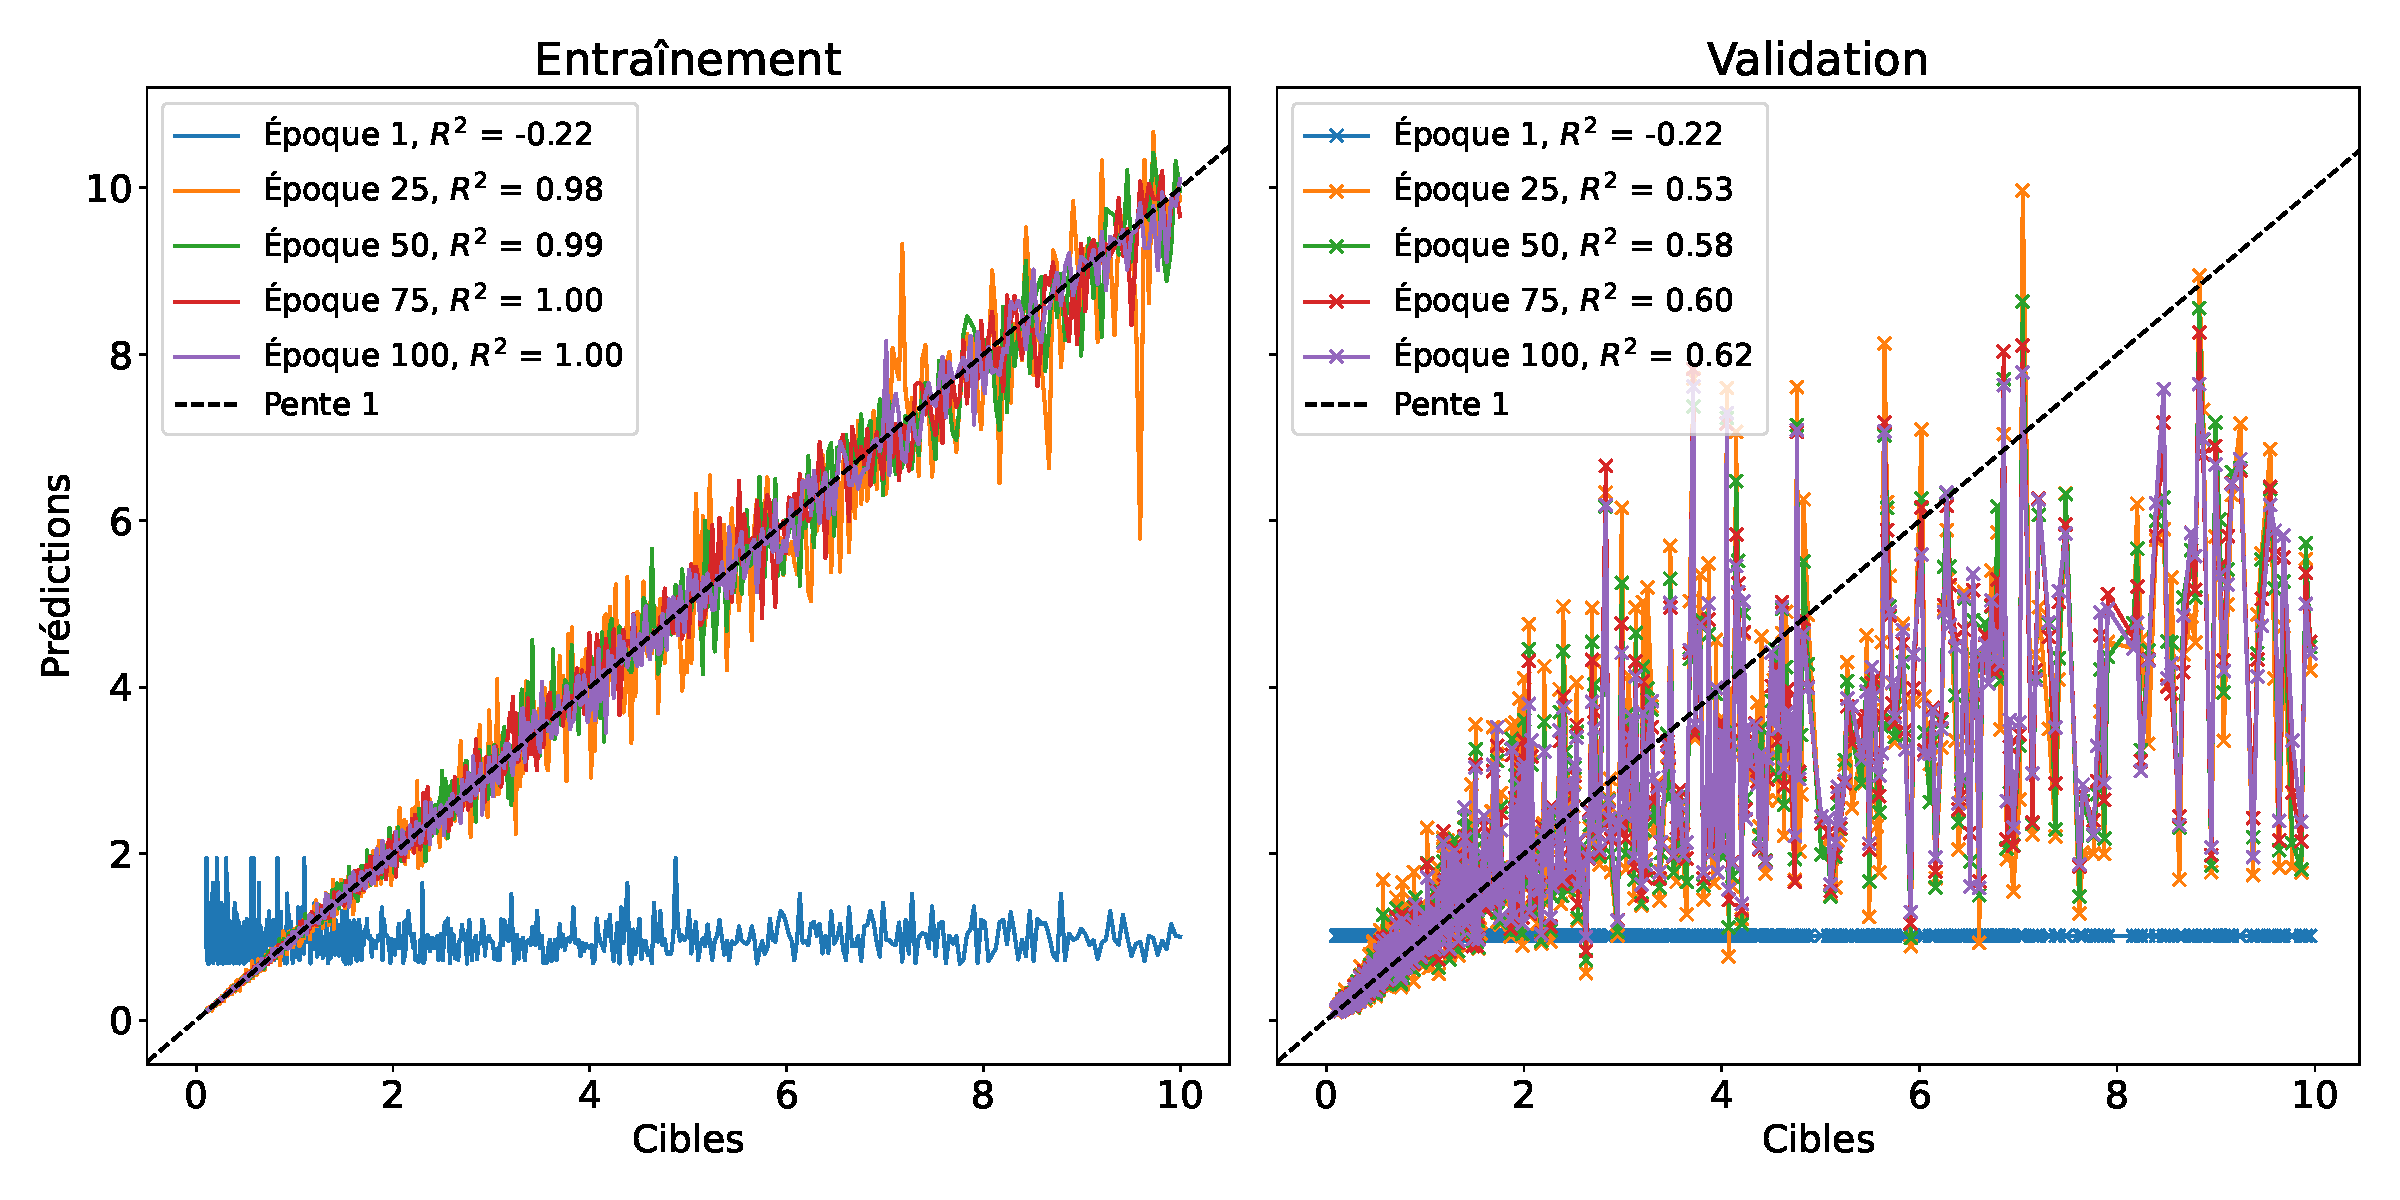
\includegraphics[width=\linewidth]{images/predsVsTargs_v3.pdf}
    \caption{Prédictions en fonction des cibles du le troisième réseau pour l'entraînement et la validation. On affiche quelques époques par graphique.}
    \label{fig:predsVsTargs_v3}
\end{figure}
\begin{figure}[h!!]
    \centering
    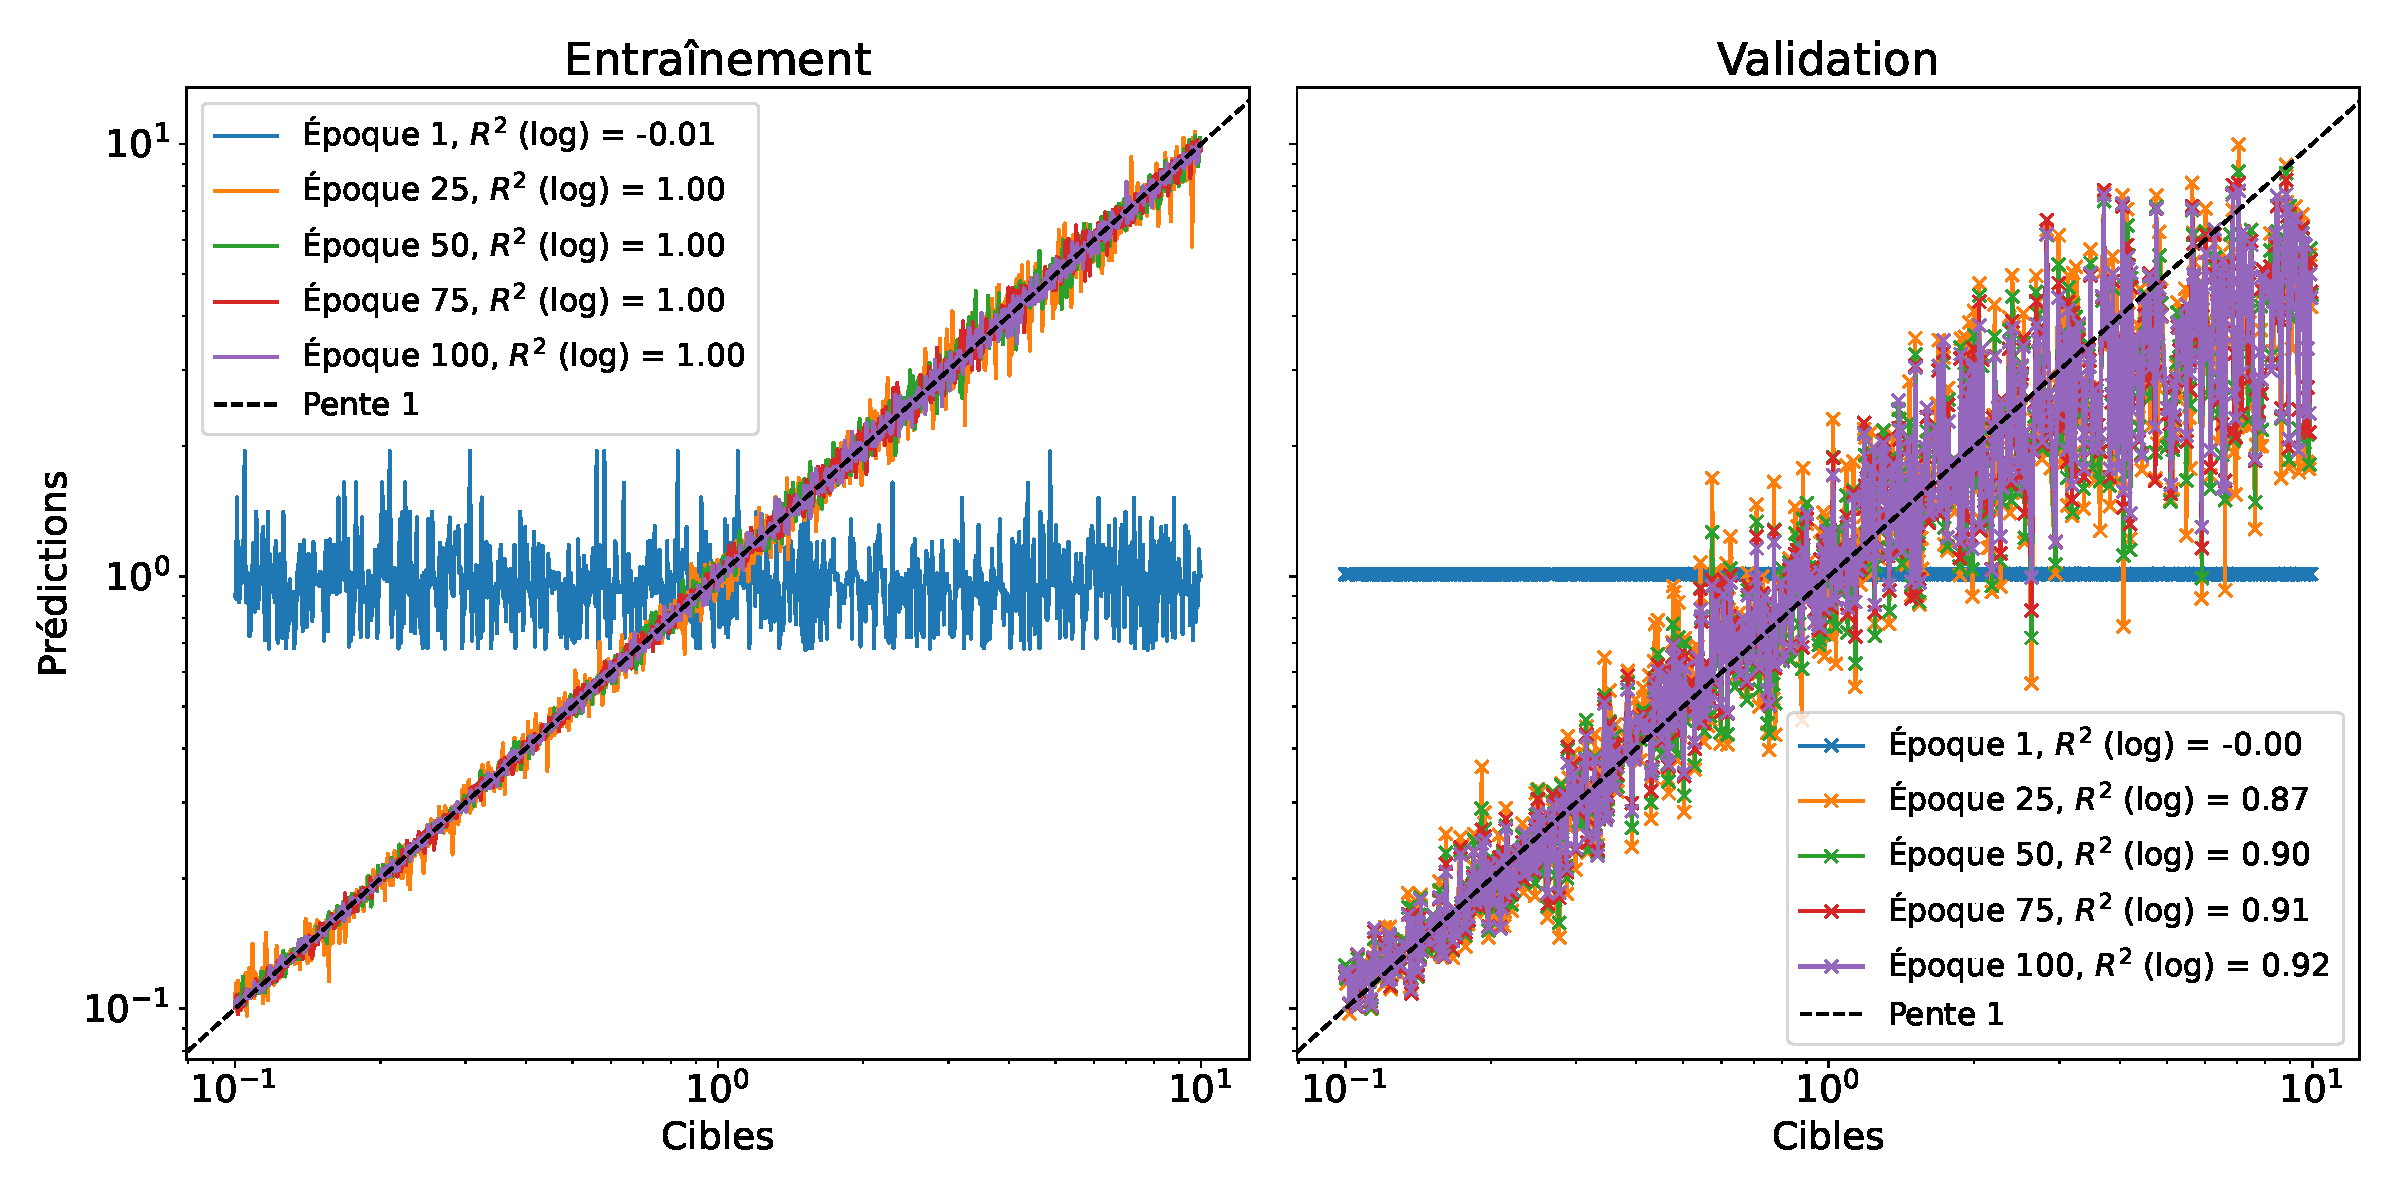
\includegraphics[width=\linewidth]{images/predsVsTargs_v3_log.pdf}
    \caption{Log-prédictions en fonction des log-cibles du le troisième réseau pour l'entraînement et la validation. On affiche quelques époques par graphique.}
    \label{fig:predsVsTargs_v3_log}
\end{figure}
On peut expliquer une partie des moins bonnes performances par l'augmentation non négligeables de temps caractéristiques dans le régime $\tau_c > T$ pour ce réseau contrairement au deux précédents. Au lieu d'avoir seulement quelques points, on y en retrouve beaucoup plus. Si les performances ne sont pas précises dans ce régime, alors augmenter le nombre de prédictions diminue la qualité générale sans surprise. Il faut alors changer des hyperparamètres du réseau, comme ce qui est fait pour le quatrième.
\newpage
\subsection{Quatrième réseau}
Pour le quatrième réseau, on prend le troisième, mais on augmente le taux d'apprentissage de $10^{-4}$ à $10^{-3}$. La perte en fonction des cibles est présentée à la figure \ref{fig:LAE_vs_tau_c_v4}. On y voit une nette amélioration en validation avec des pertes plus souvent sous la barre de $0.1$, mais ayant encore la remontée pour $\tau_c$ qui augmente.
\begin{figure}[h!!]
    \centering
    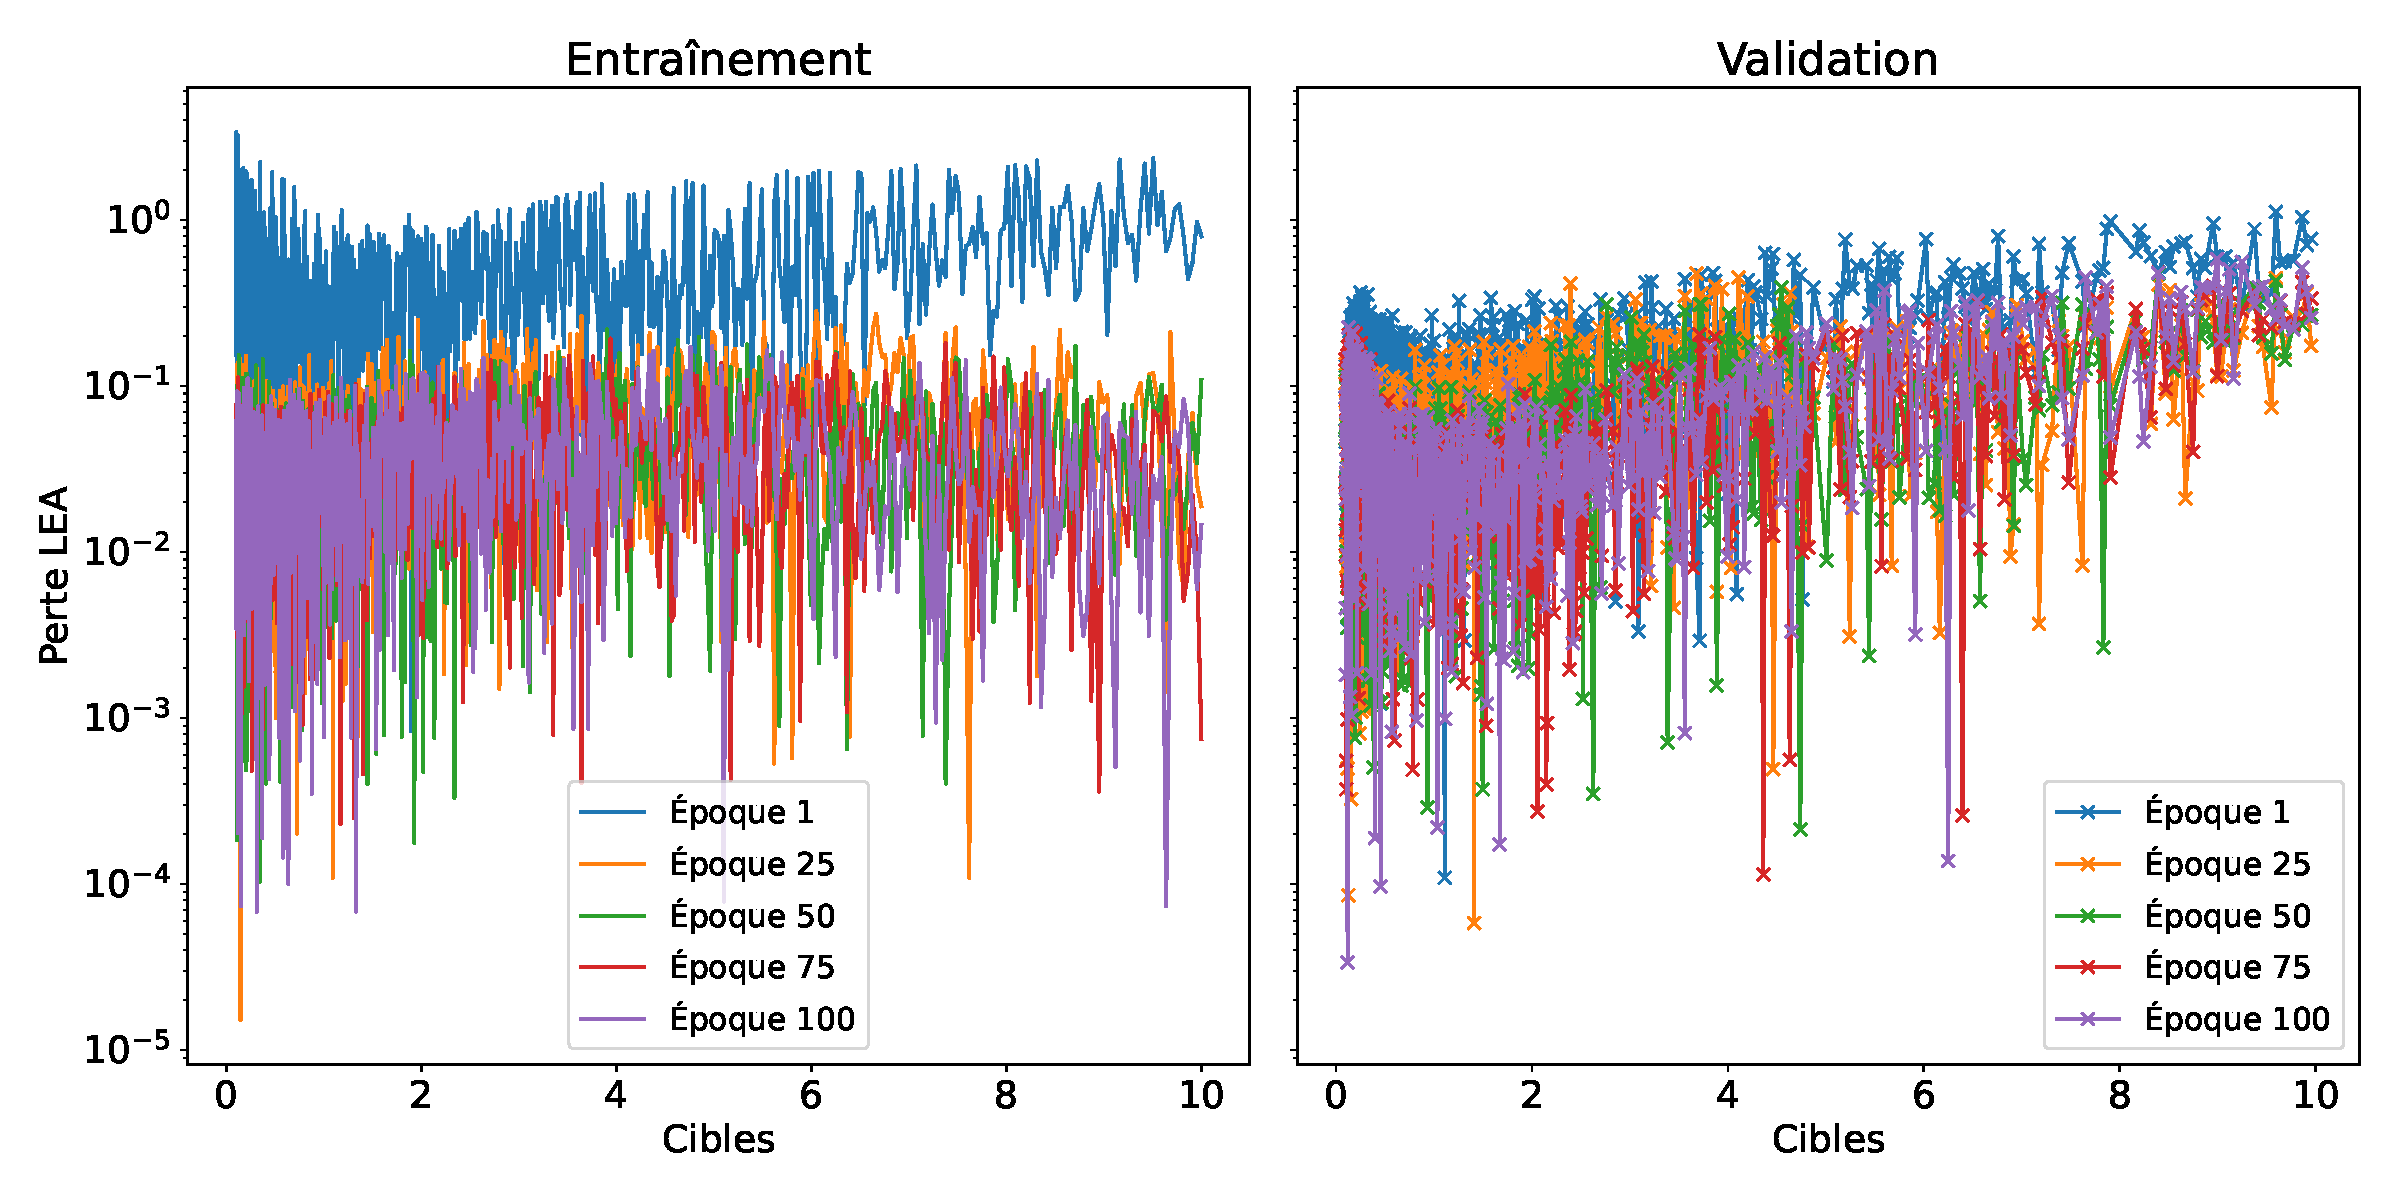
\includegraphics[width=\linewidth]{images/LAEVsTargs_v4.pdf}
    \caption{Perte log erreur absolue du quatrième réseau en fonction des cibles pour l'entraînement et la validation. On affiche quelques époques par graphique.}
    \label{fig:LAE_vs_tau_c_v4}
\end{figure}
La meilleure précision se voit aussi dans la figure \ref{fig:predsVsTargs_v4} où les coefficients de déterminations arrivent rapidement à surpasser $0.9$, la linéarité étant meilleure. Pour l'échelle logarithmique, on s'approche de l'unité, tel que montré à la figure \ref{fig:predsVsTargs_v4}. Bien qu'il y ait encore une certaine difficulté pour le régime $\tau_c > T$, augmenter le taux d'apprentissage rend cette difficulté plus facile à assimiler.
\begin{figure}[h!!]
    \centering
    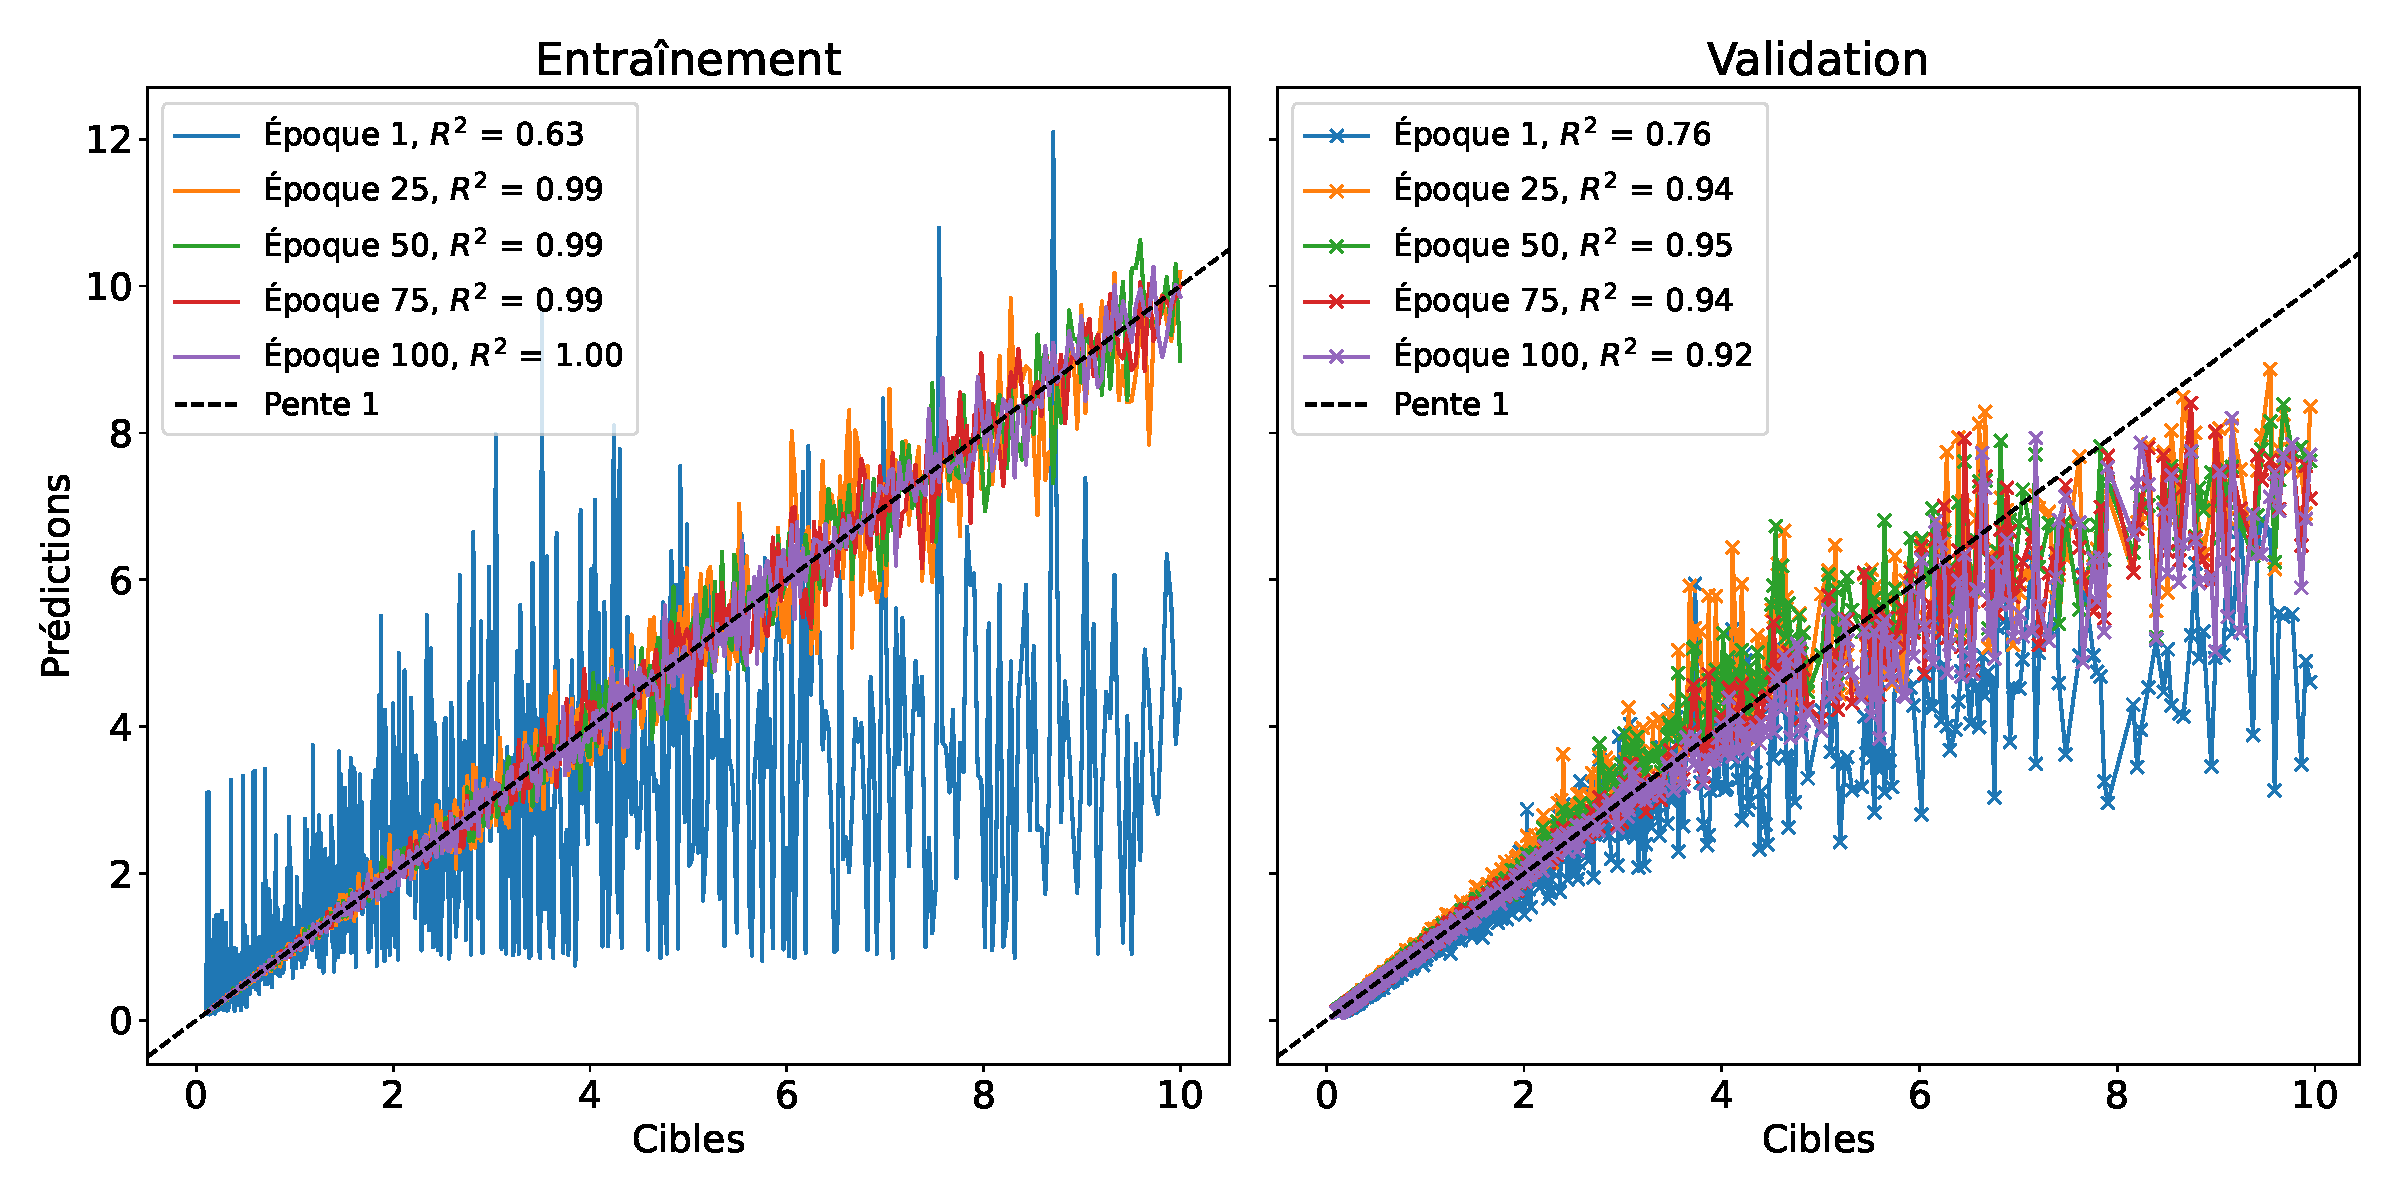
\includegraphics[width=\linewidth]{images/predsVsTargs_v4.pdf}
    \caption{Prédictions en fonction des cibles du le quatrième réseau pour l'entraînement et la validation. On affiche quelques époques par graphique.}
    \label{fig:predsVsTargs_v4}
\end{figure}
\newpage
\begin{figure}[h!!]
    \centering
    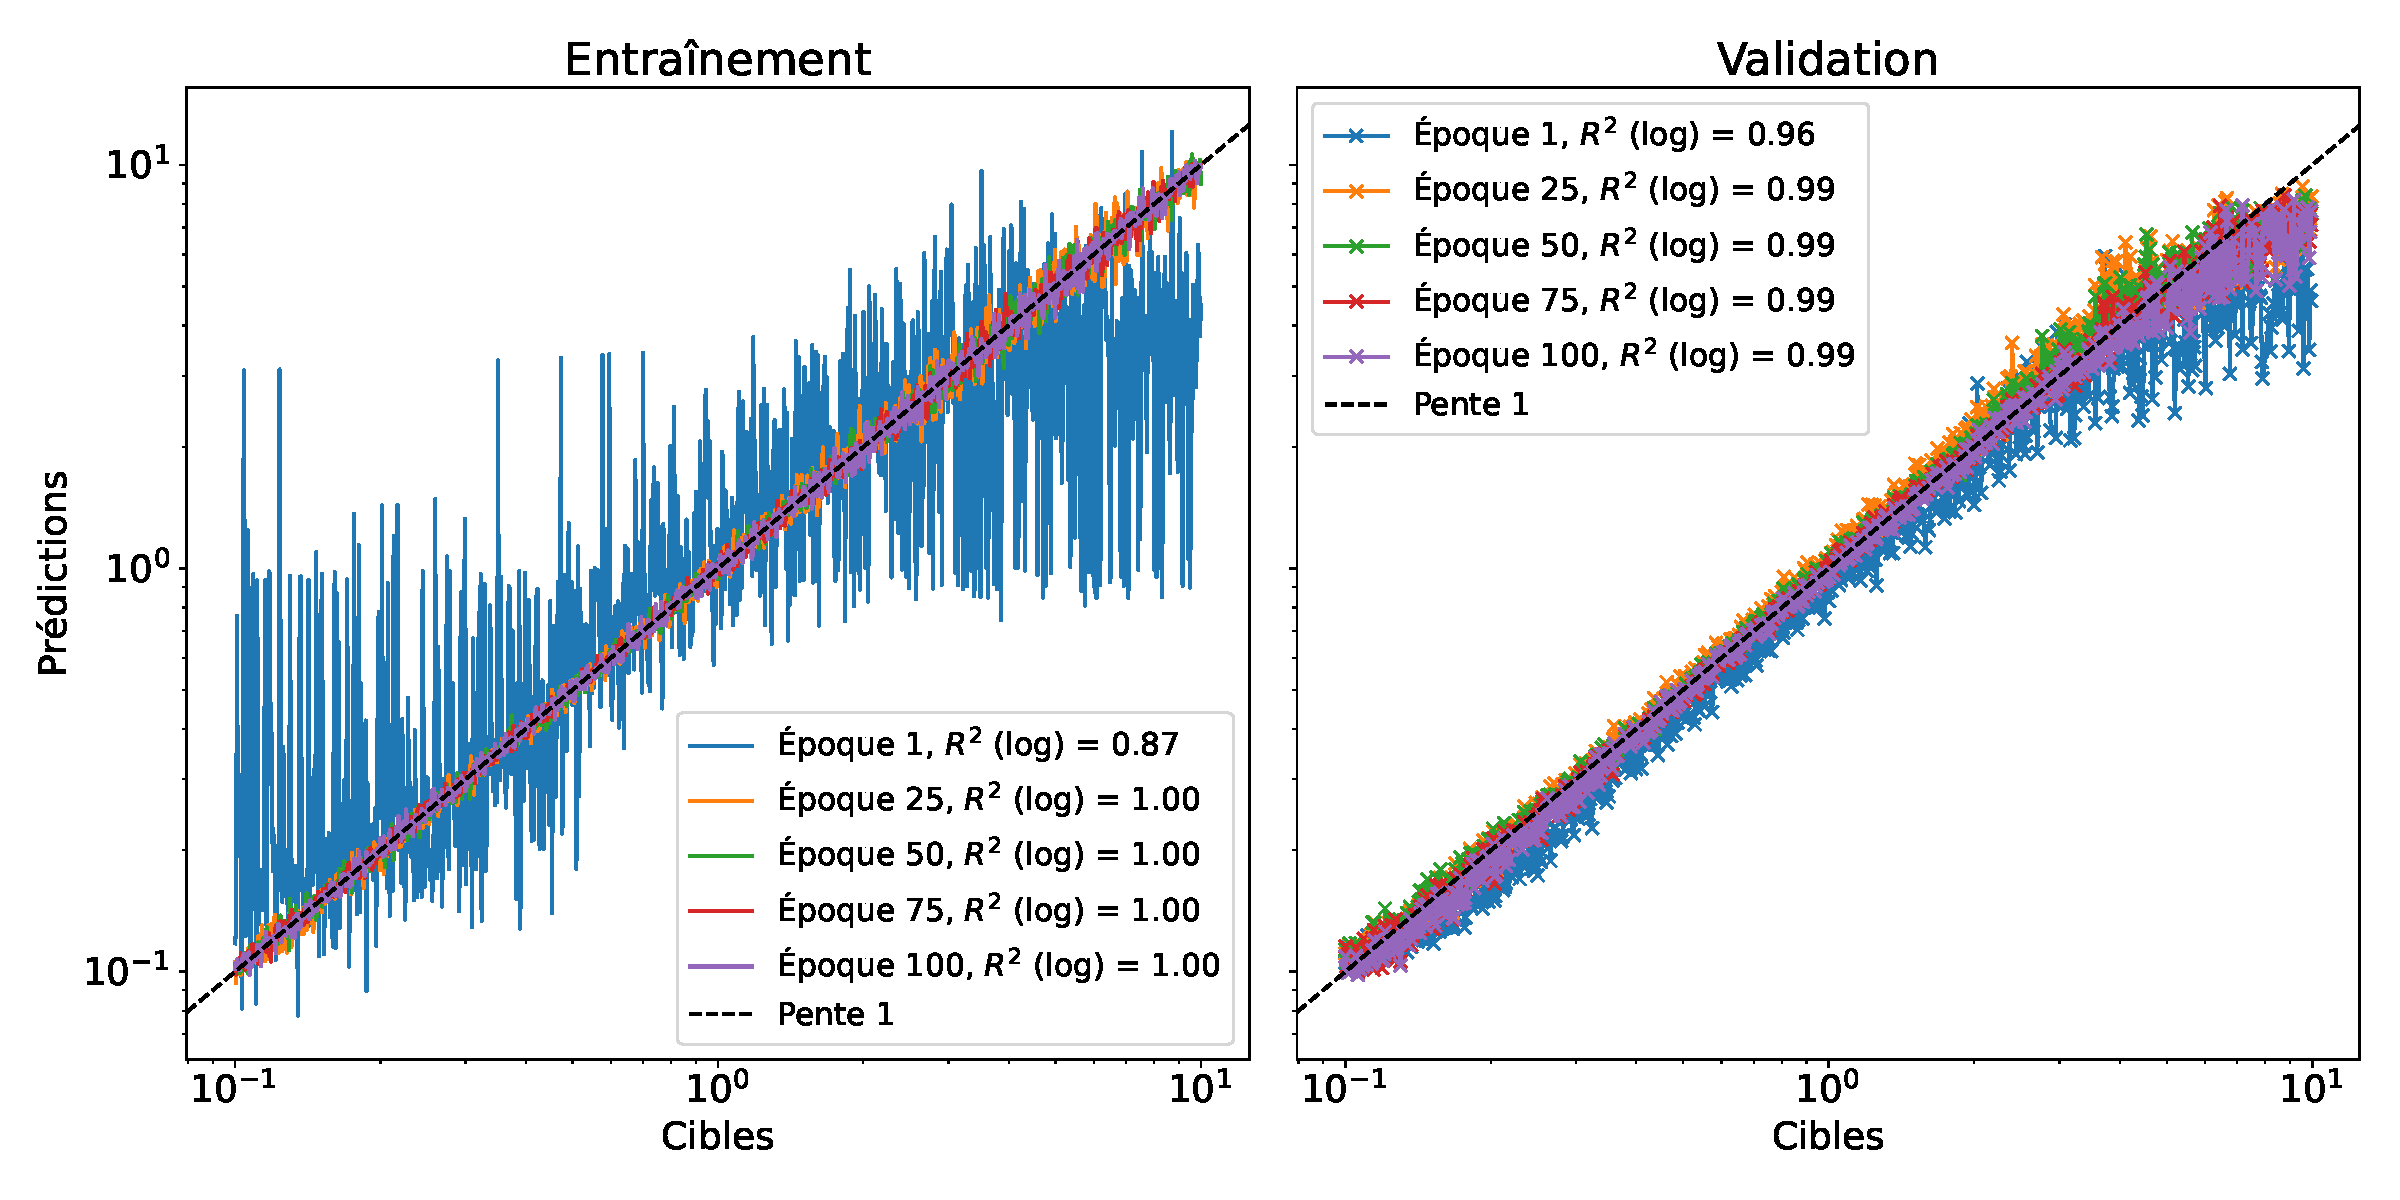
\includegraphics[width=\linewidth]{images/predsVsTargs_v4_log.pdf}
    \caption{Log-prédictions en fonction des log-cibles du le quatrième réseau pour l'entraînement et la validation. On affiche quelques époques par graphique.}
    \label{fig:predsVsTargs_v4_log}
\end{figure}
\newpage
\subsection{Cinquième réseau}
Pour le dernier réseau présenté, on se base sur le troisième et le quatrième, mais avec un taux de $5\times 10^{-4}$. Les courbes d'apprentissage semblaient indiquer que le réseau était dans les meilleurs, ce qui est aussi remarqué à la figure \ref{fig:LAE_vs_tau_c_v5}, soit la perte en fonction des cibles. Le régime $\tau_c < T$, ainsi que le régime $\tau_c\approx T$ sont souvent sous la barre de $0.01$ de perte, alors que le régime $\tau_c > T$ semble plus stable et varier légèrement autour de $0.1$.
\begin{figure}[h!!]
    \centering
    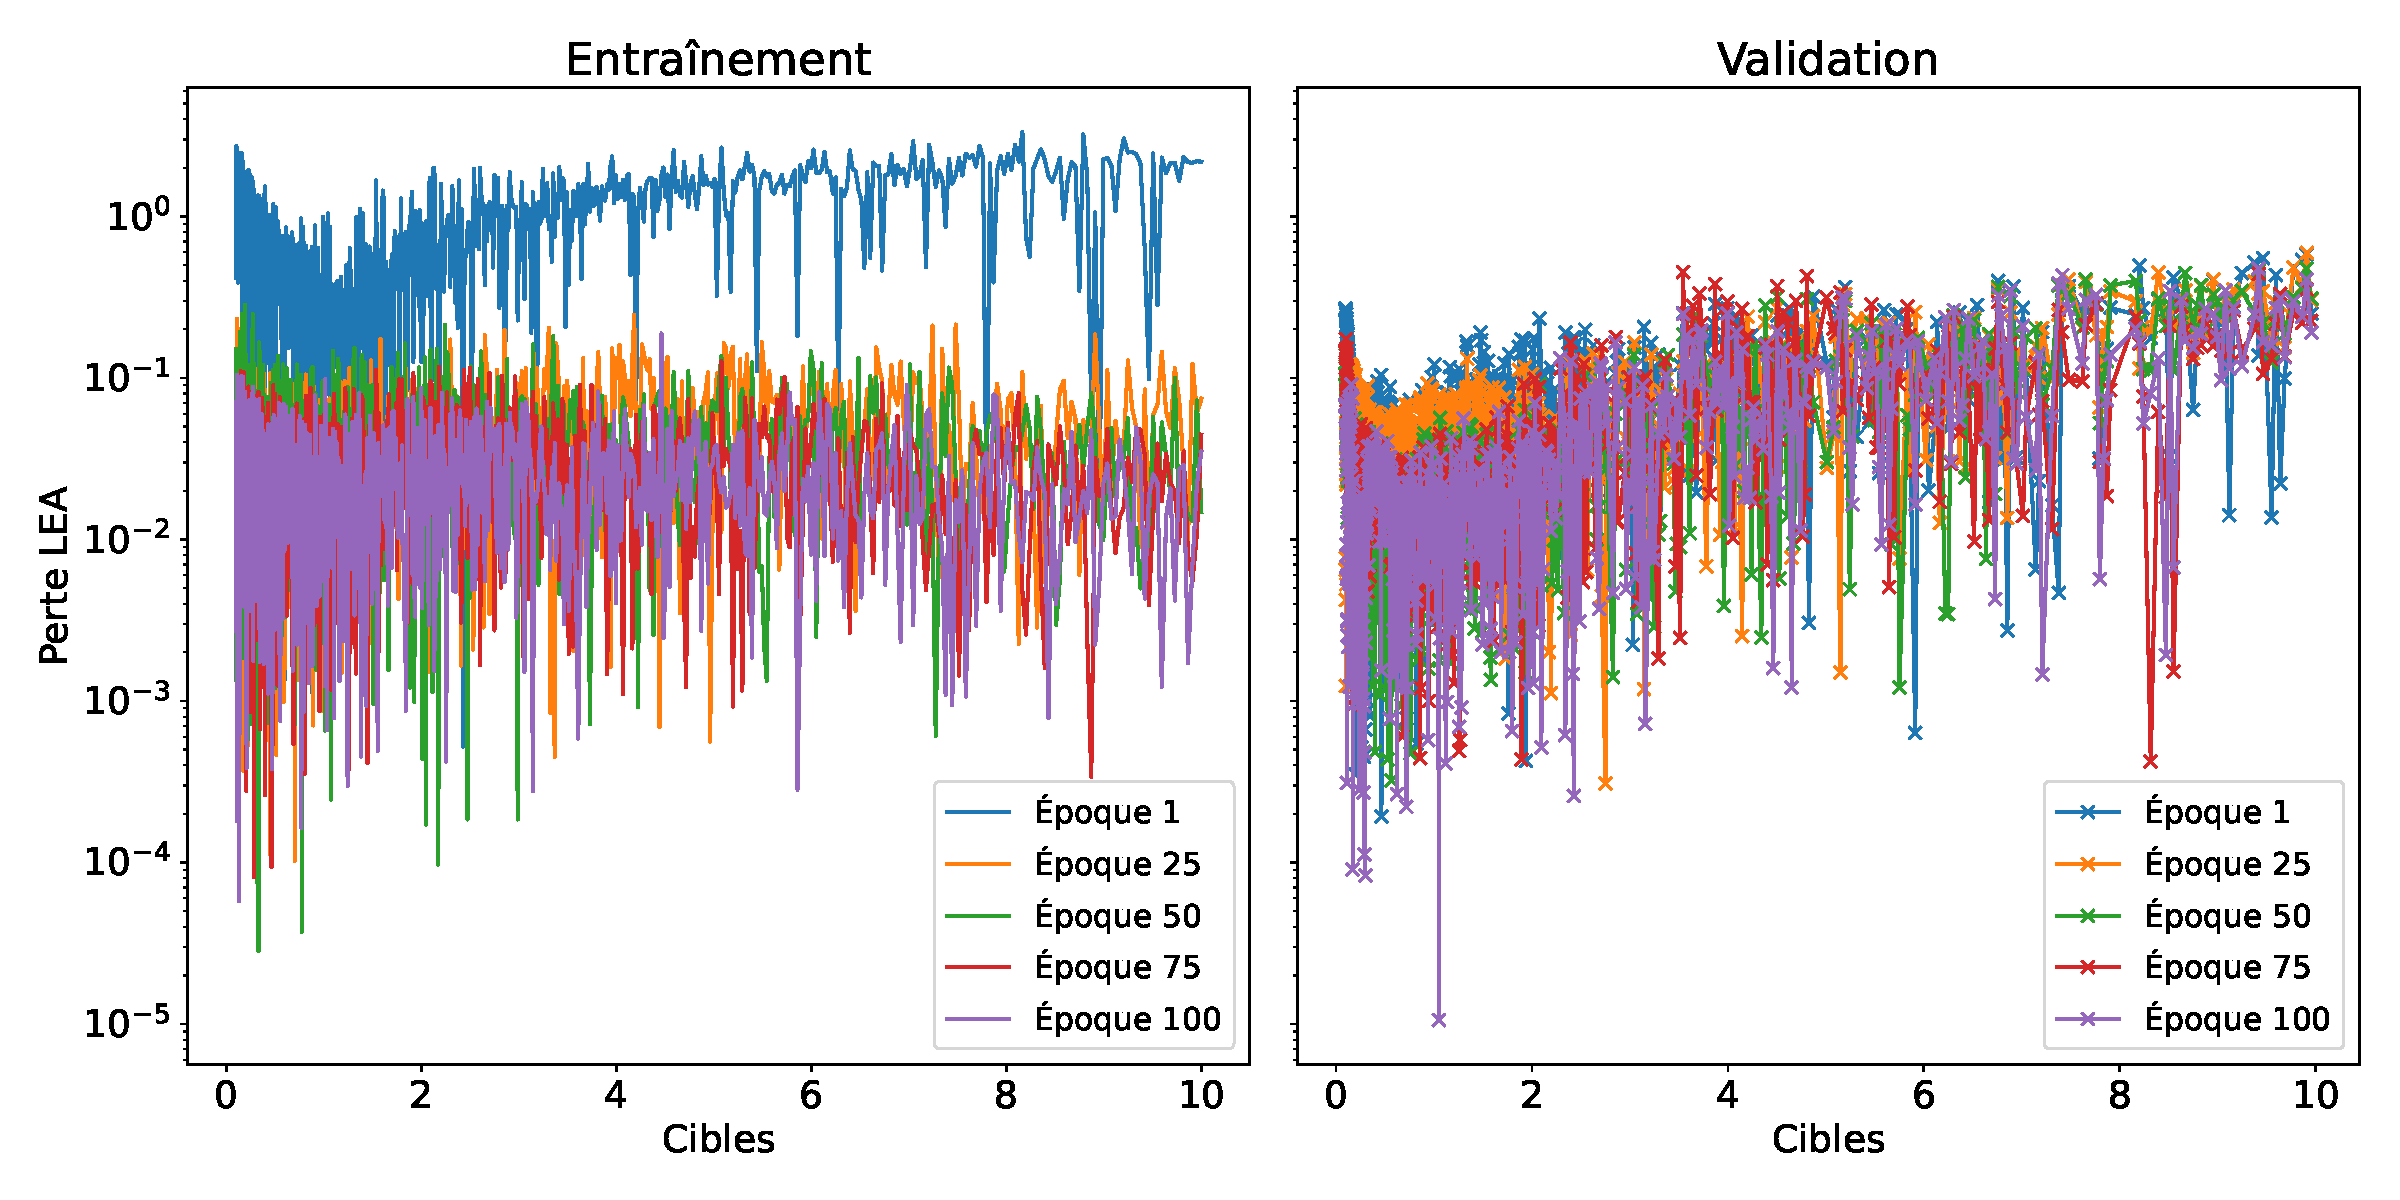
\includegraphics[width=\linewidth]{images/LAEVsTargs_v5.pdf}
    \caption{Perte log erreur absolue du cinquième réseau en fonction des cibles pour l'entraînement et la validation. On affiche quelques époques par graphique.}
    \label{fig:LAE_vs_tau_c_v5}
\end{figure}
À la figure \ref{fig:predsVsTargs_v5}, on voit que les predictions restent proches des cibles sur un intervalle de $\tau_c$ plus grand, déviant plus lentement et à plus petite amplitude que pour les réseaux précédents, idem pour la figure en échelle logarithmique, la figure \ref{fig:predsVsTargs_v5_log}. On est plus centré sur la diagonale, et ce avec une variance plus faible.
\newpage
\begin{figure}[h!!]
    \centering
    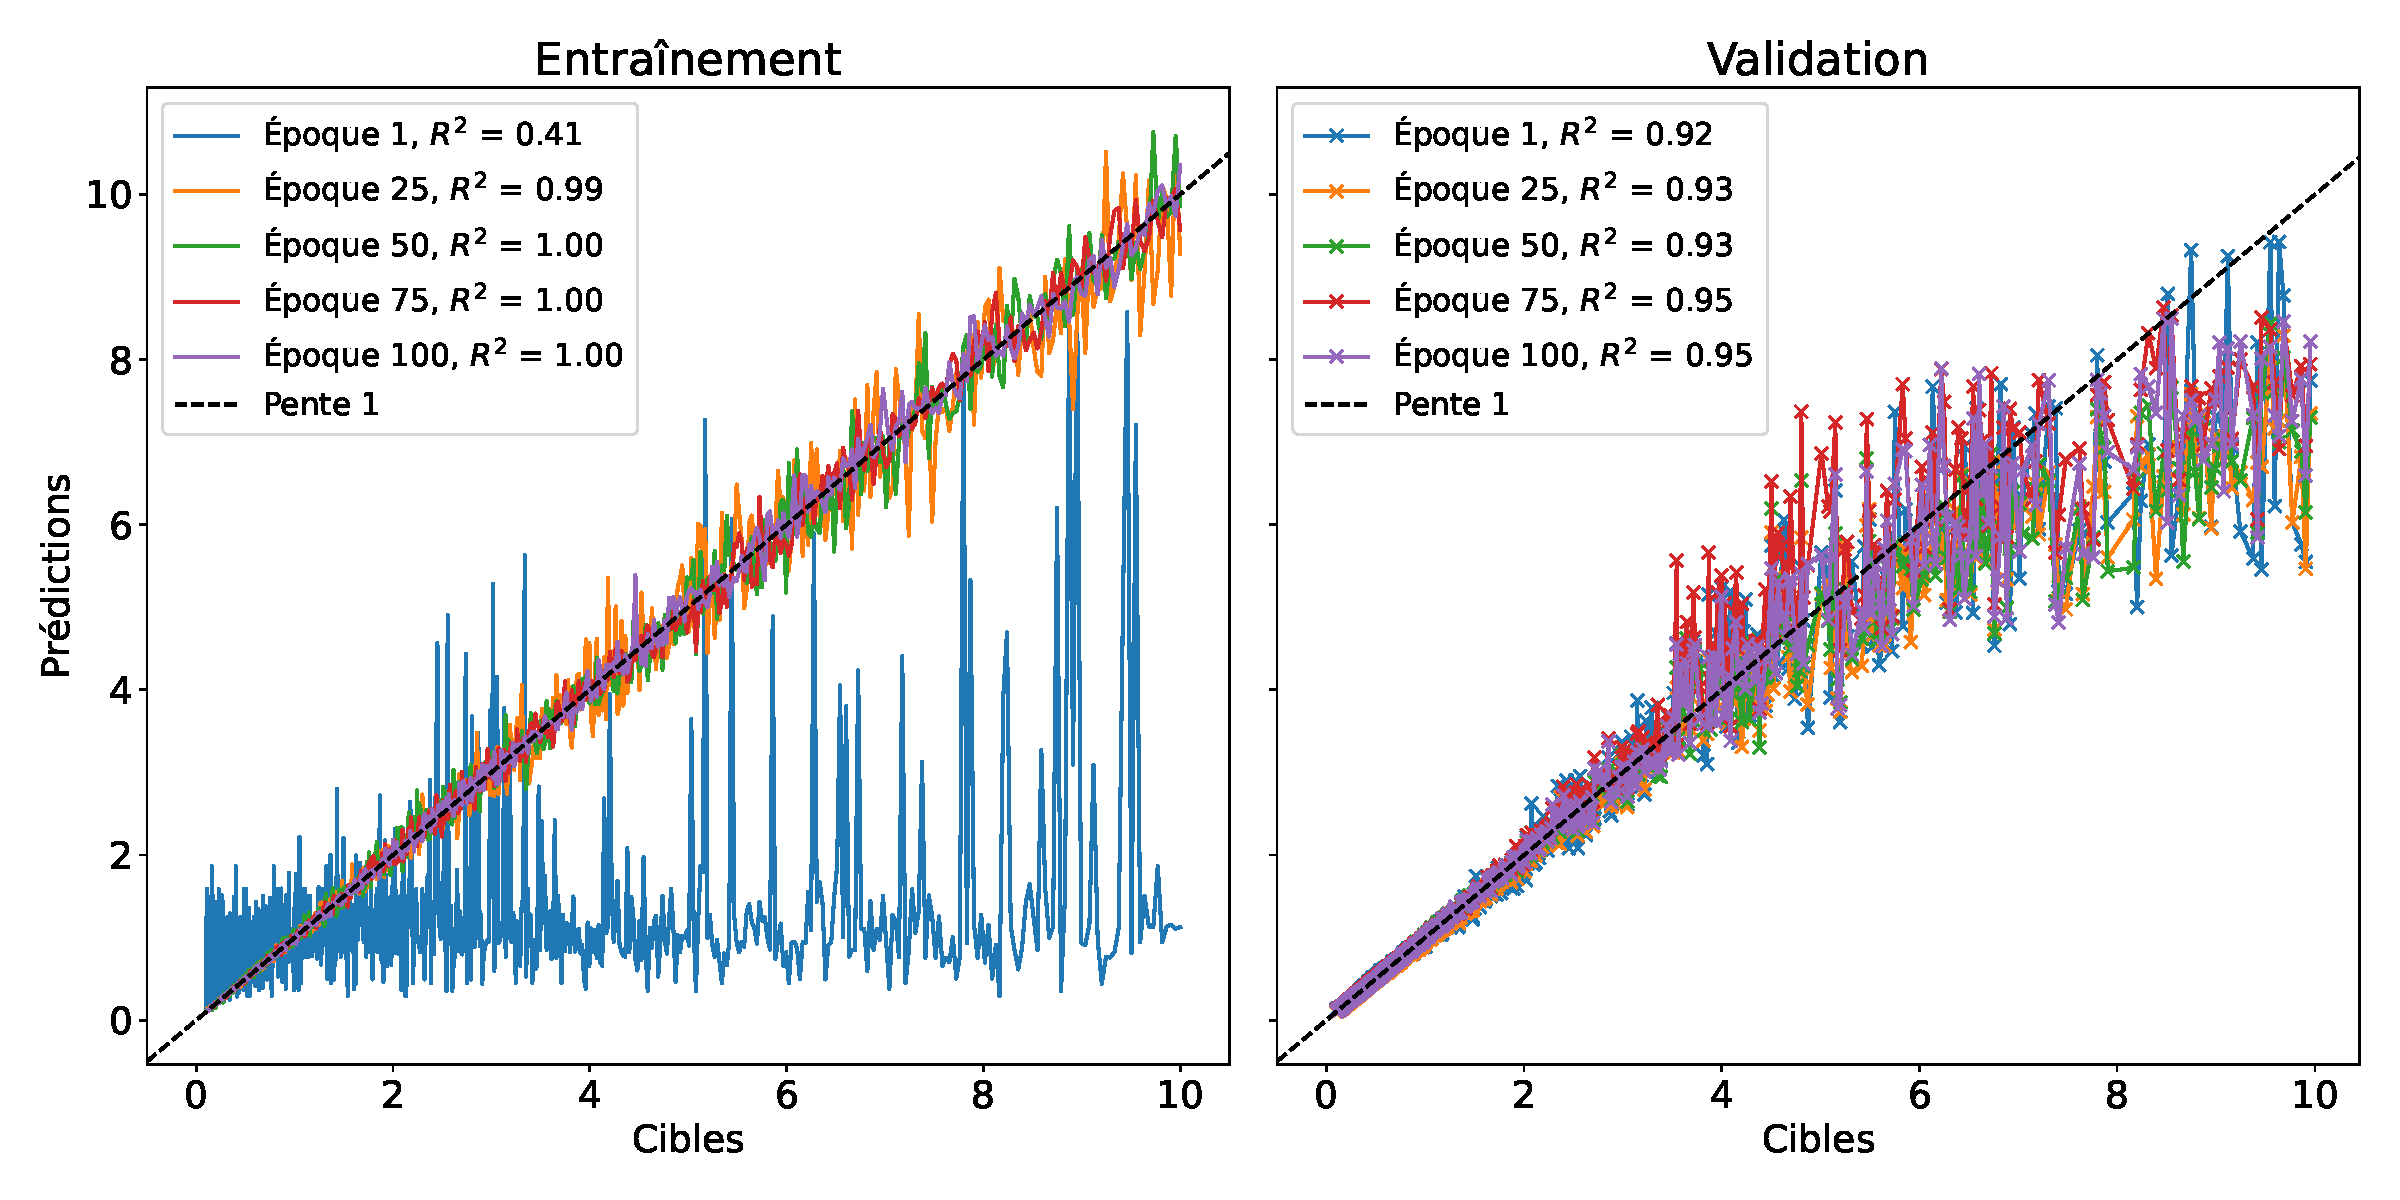
\includegraphics[width=\linewidth]{images/predsVsTargs_v5.pdf}
    \caption{Prédictions en fonction des cibles du le cinquième réseau pour l'entraînement et la validation. On affiche quelques époques par graphique.}
    \label{fig:predsVsTargs_v5}
\end{figure}
\begin{figure}[h!!]
    \centering
    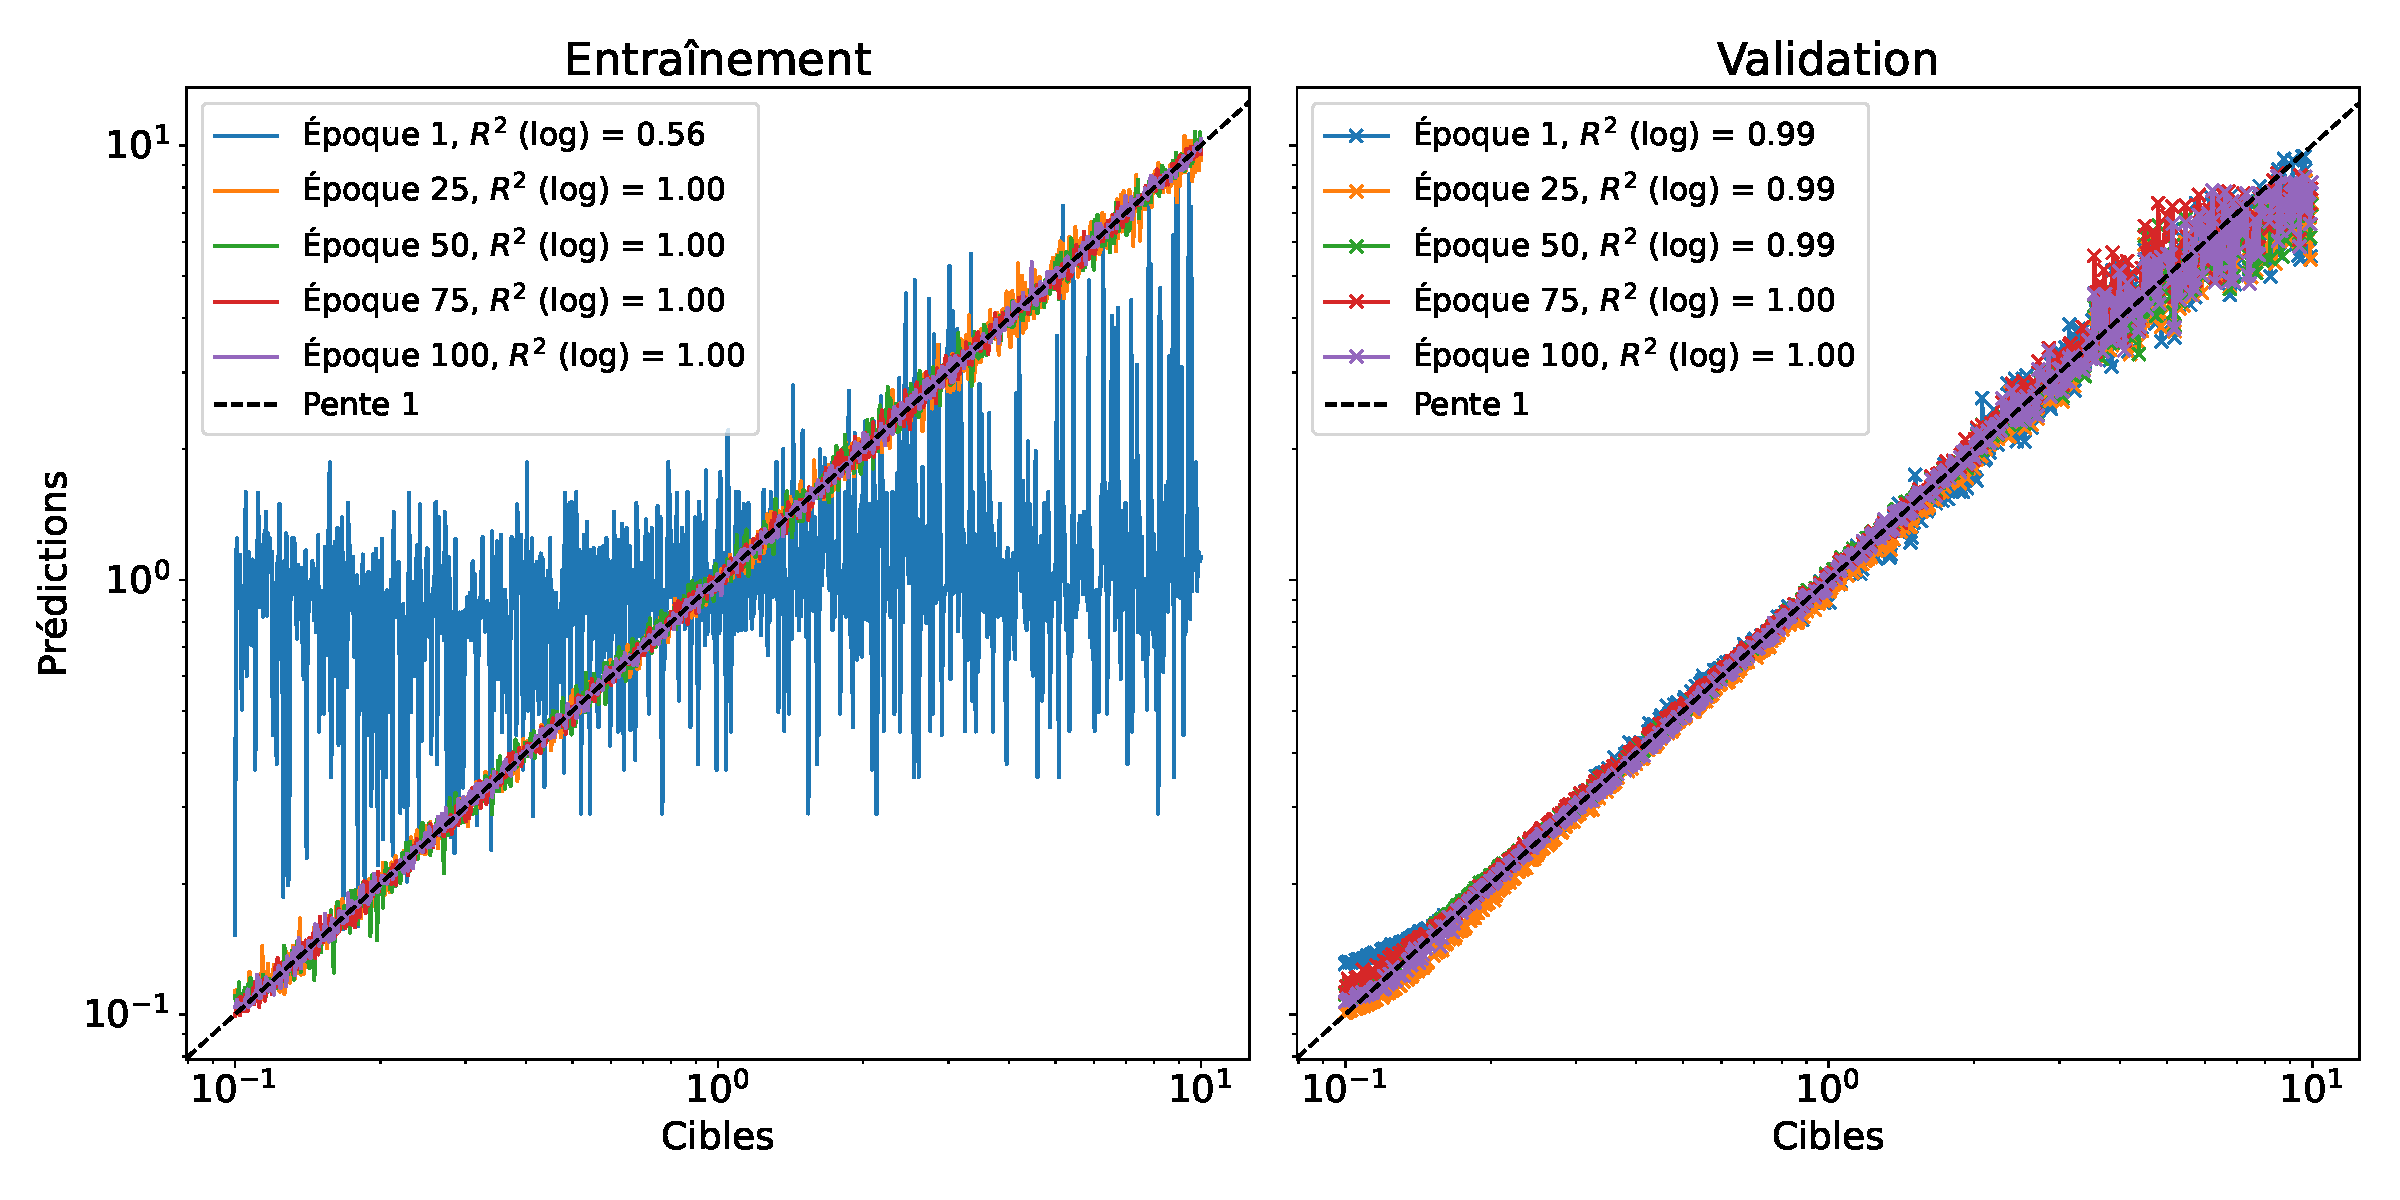
\includegraphics[width=\linewidth]{images/predsVsTargs_v5_log.pdf}
    \caption{Log-prédictions en fonction des log-cibles du le cinquième réseau pour l'entraînement et la validation. On affiche quelques époques par graphique.}
    \label{fig:predsVsTargs_v5_log}
\end{figure}
\newpage
\section{Analyses supplémentaires}
Dans tous les cas étudiés jusqu'à présent, on note une difficulté à traiter les cas où les cibles sont plus élevées que le temps d'intégration. Deux explications indépendantes peuvent être expliquées. Premièrement, en générant les temps caractéristiques sur une échelle logarithmique, on met l'emphase sur les petites valeurs, obtenant plus de $\tau_c$ dans les régimes $\tau_c < T$ et $\tau_c \approx T$. Cela peut créer un débalancement dans les données, donc un apprentissage moins efficace dans les cas éloignés de $\tau_c > T$. Le choix de l'échelle logarithmique n'est pas anodin. Dans la physique des tavelures, on retrouve plus souvent des cas $\tau_c < T$, car la décorrélation des matériaux se fait plus rapidement que l'intégration ou l'accumulation des pixels dans une caméra. Plus $\tau_c$ surpasse $T$, plus c'est un régime biologique rare, sauf si on s'intéresse à des surfaces rigides. Dans le cas biomédical, on reste souvent dans le cas $\tau_c < T$ ou $\tau_c \approx T$.
\\ \\
Deuxièmement, les réseaux utilisent des couches de convolutions 2D qui déterminent les caractéristiques importantes pour la partie récurrente. Ces convolutions n'ont accès qu'aux pixels d'une même image, ils n'ont pas de références explicitent au temps. On sait toutefois dans la physique des tavelures que le contraste spatial, soit $C = \frac{\sigma}{\mu}$ où $\sigma$ est l'écart-type d'intensité et $\mu$ en est la moyenne, dépend implicitement des propriétés temporelles. Dans le cas d'une corrélation temporelle exponentielle, on a la formule\cite{monMemoire}
\begin{align*}
C = \sqrt{\beta\frac{\tau_c}{2T}\left[2 + \frac{\tau_c}{T}\left(\exp{-\frac{2T}{\tau_c}} - 1\right)\right]}
\end{align*}
où $\tau_c$ est le temps caractéristique, $T$ est le temps d'intégration et $\beta$ est un paramètre qu'on va supposer égal à $1$. La figure \ref{fig:contrast_fct_tau_c} montre cette formule graphiquement, mais avec $T = 1$.
\begin{figure}[h!!]
    \centering
    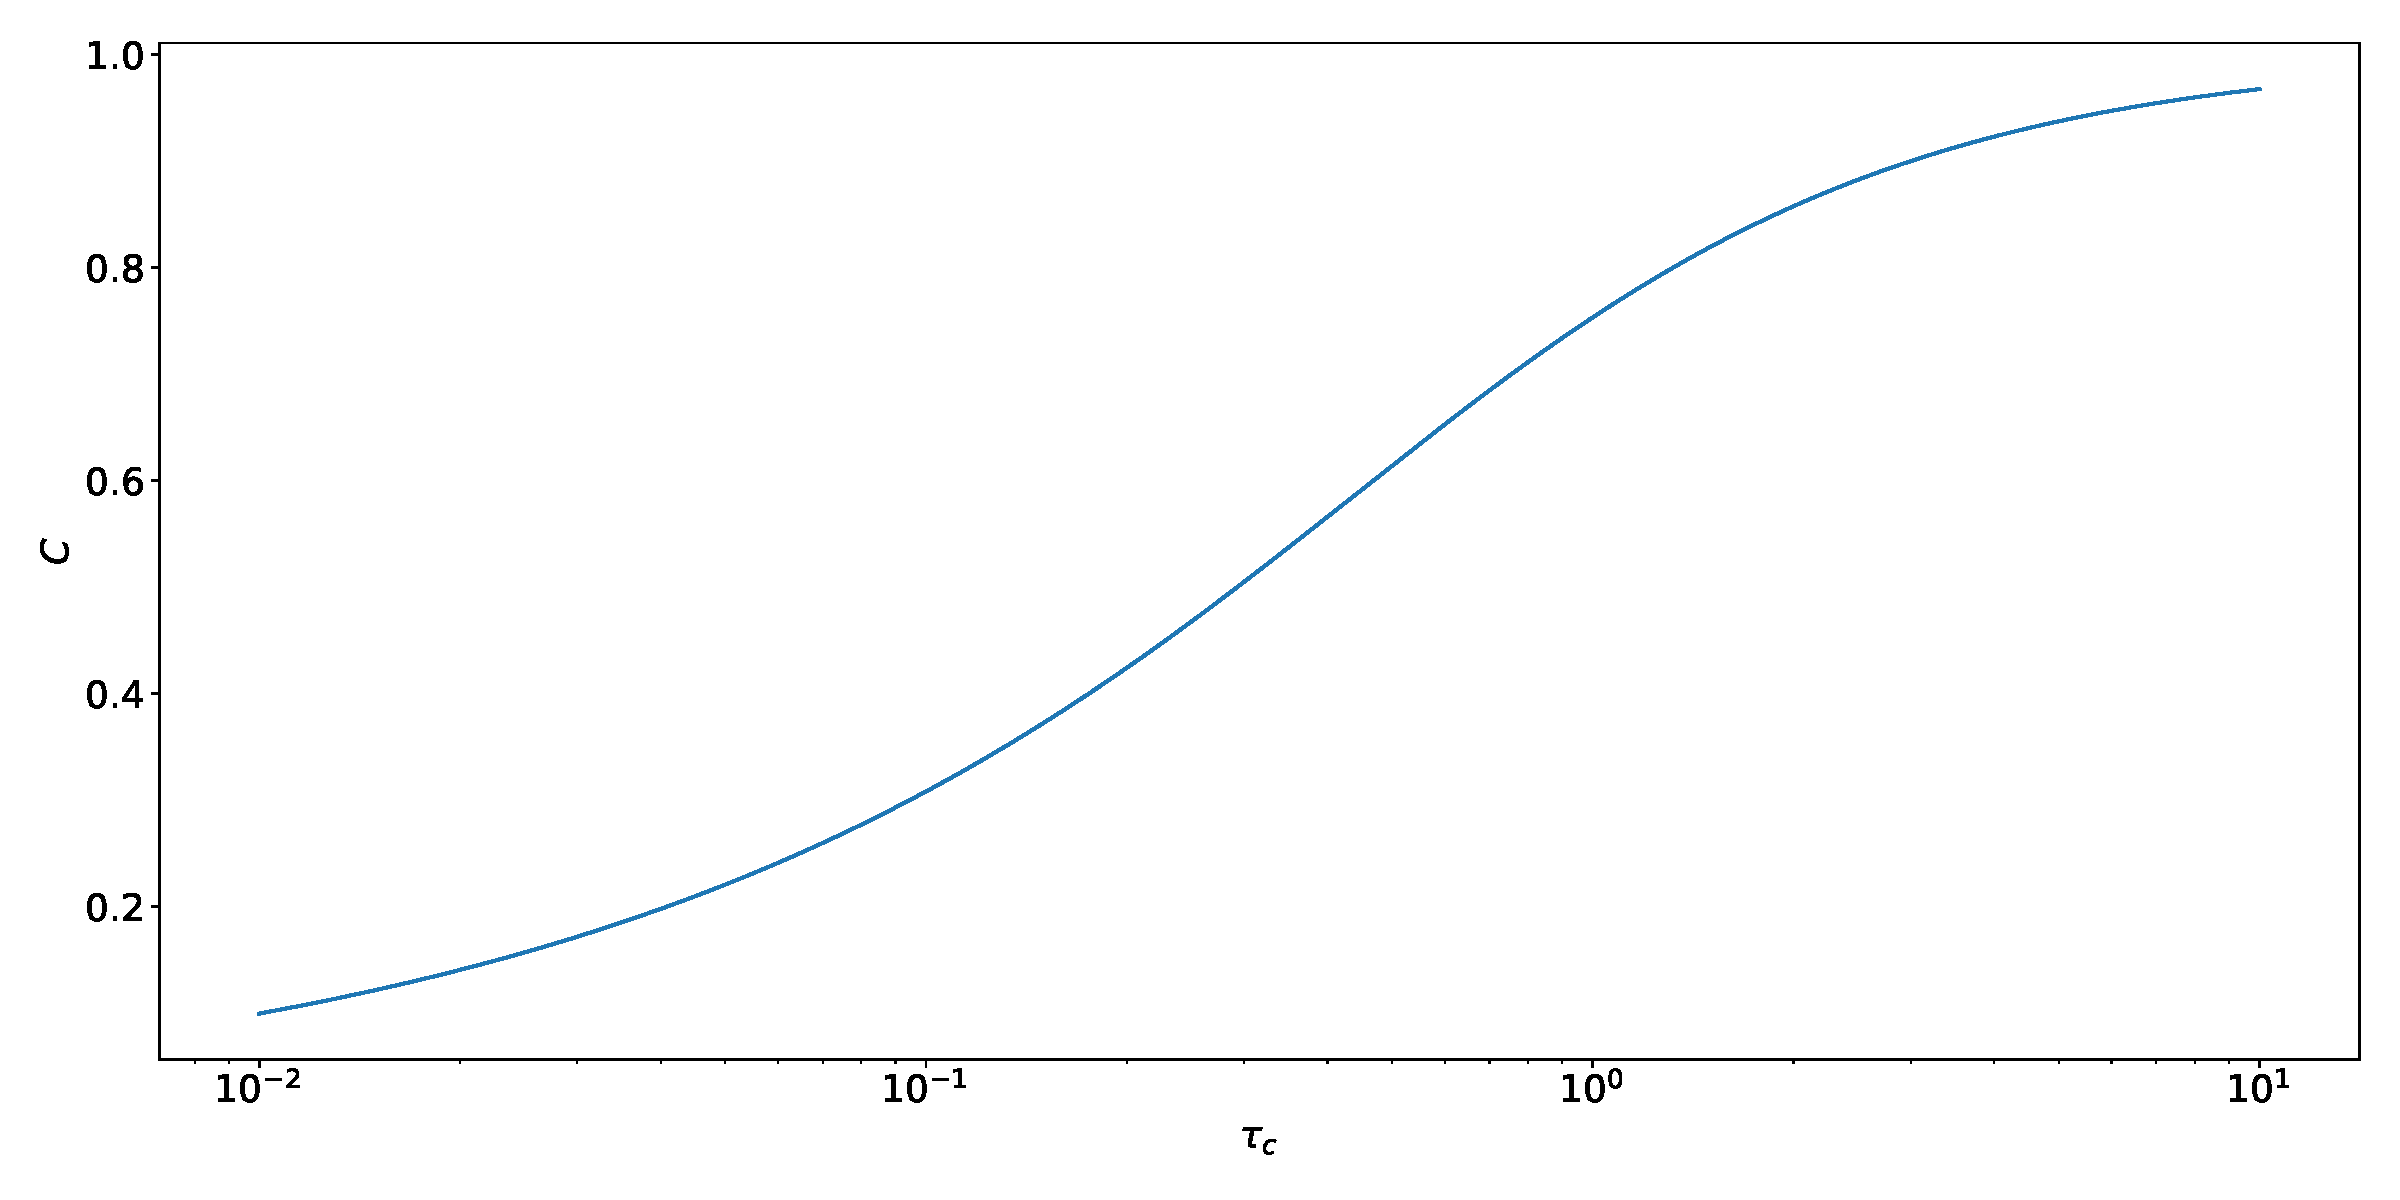
\includegraphics[width=0.95\linewidth]{images/contrast_fct_tau_c.pdf}
    \caption{Contraste spatial en fonction du temps caractéristique $\tau_c$ pour un temps d'intégration constant à $1$.}
    \label{fig:contrast_fct_tau_c}
\end{figure}
Plus $\tau_c$ augmente, plus le contraste approche $1$ en asymptote, donc peu importe $\tau_c$, le contraste reste proche de $1$ et ne donne plus beaucoup d'information à propos de la corrélation temporelle. Dans le régime $\tau_c \approx T$, on a un contraste croissant rapidement en fonction de $\tau_c$, donc beaucoup d'information à propos de la corrélation. Finalement, dans le cas $\tau_c < T$, on a aussi une asymptopte à $0$, donc si le temps caractéristique devient beaucoup plus petit que $T$, le contraste, un fois de plus, n'apporte pas d'information sur la corrélation temporelle. C'est ce qui pourrait expliquer les petites divergences dans les figures prédictions en fonction des cibles en échelle logarithme pour les petits $\tau_c$. La figure \ref{fig:contrastDiffDiffTauC}, tirée de \cite{monMemoire}, montre graphiquement que lorsque le ratio $T/\tau_c$ change, la différence de contraste devient plus ou moins évidente, donc renferme plus ou moins d'information. On voit que la différence de contraste est maximale lorsque $T$ est proche des temps caractéristiques impliqués.
\begin{figure}[h!!]
    \centering
    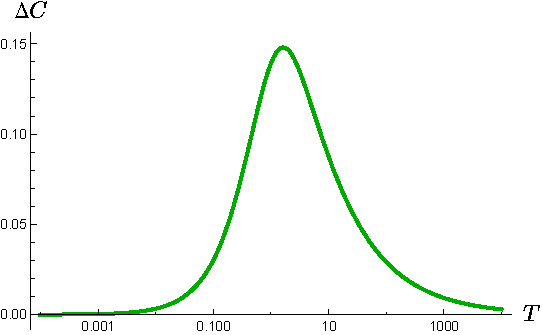
\includegraphics[width=\linewidth]{images/contrastDiffDiffTauC.pdf}
    \caption{Différence de contraste spatial en fonction du temps d’acquisition entre des tavelures corrélées exponentiellement avec $\tau_c = 0.5$ et $\tau_c = 1$.}
    \label{fig:contrastDiffDiffTauC}
\end{figure}
\newpage
\chapter{Seconde partie du projet}
Dans la seconde moitié de la session, il sera question d'optimiser le réseau. On sait qu'il est possible d'apprendre et de généraliser sous certaines conditions. Il sera important de varier les conditions et d'augmenter la complexité. L'évaluation finale se fera ainsi à ce moment.
\section{Optimisation}
Dans le chapitre précédent, différentes architectures et différents hyperparamètres sont testés. Le dernier est le plus prometteur, mais il est peut-être possible d'en avoir un meilleur. Il peut être important d'effectuer une recherche d'hyperparamètres, comme le taux d'apprentissage, le nombre de couches de convolution, leurs tailles, leurs nombres de filtres, ainsi que la partie récurrente avec le nombre de couches GRU et le nombre d'unités cachées. De plus, il serait intéressant de tester l'ajout de composants qui sont normalement présent dans la plupart des architectures CNN, comme une normalisation entre les couches. Il ne sera pas question de \textit{batch norm} ici, car la structure d'une batch peut contenir différentes séquences temporelles indépendantes et on mélangerait ainsi les statistiques, brouillant l'information. \textit{Instance norm} est considéré. Dans la plupart des cas, ajouter une couche de normalisation aide la convergence. Finalement, éventuellement il serait important d'ajouter une couche de normalisation $[0, 1]$ en entrée du réseau, permettant de mettre toutes les images à la même échelle dans l'intervalle $[0, 1]$. Contrairement à une normalisation $z-score$, on ne modifie pas vraiment la nature des distributions de probabilité, on ne fait que les translater dans un certain intervalle.
\section{Varier les conditions}
On s'est pour l'instant seulement intéressé à une fonction de corrélation et un seul temps d'intégration lors des tests présentés dans le chapitre \ref{resultats_initiaux}. Or, n'avoir qu'un seul temps d'intégration n'est pas critique, car c'est le ratio $T/\tau_c$ qui joue un rôle primordial dans les statistiques spatiales, comme le contraste. En faisant varier $\tau_c$ seulement, on fait varier ce ratio sans avoir de temps d'intégration qui varie. Il serait toutefois intéressant de tester si le réseau entraîné sur, par exemple $T = 1$ performe aussi bien sur des données avec $T = 2$ et des ratios identiques. Ajouter différentes fonctions de corrélation est intéressant, car on peut vérifier la robustesse du réseau à prédire le temps de corrélation même si elle est structurellement différentes. Cela est point important vers l'obtention d'un modèle d'analyse demandant le moins de paramètres possibles, comme la fonction de corrélation qui est plus souvent qu'autrement inconnue.
\\ \\
Finalement, on peut aussi penser à ajouter un masque gaussien qui vient atténuer l'intensité plus on s'éloigne du centre de l'image. Cela permet de simuler des images plus réalistes où l'illumination n'est pas uniforme sur toute l'image, par exemple un laser qui illumine seulement un tache à profil gaussien.
\section{Sélection d'un modèle scalaire final}
On a effectuée une certaine analyse d'apprentissage et de généralisation dans le chapitre \ref{resultats_initiaux}. Il est important de bâtir sur cette analyse, notamment en testant la cohérance de prédiction. Si on donne en test plusieurs séquences ayant la même cible, il est important de déterminer si les prédictions sont similaires. La cohérence d'un réseau est primordiale, sinon il ne vaut rien.
\section{Modèle cartographique: un aperçu}
Si le temps le permet, il serait intéressant d'évaluer la pertinence et la faisabilité d'un réseau cartographique. Au lieu de donner un scalaire comme sortie (ce qui est le cas dans la première partie), le réseau prédirait une carte locale de temps caractéristique. Cette approche est très intéressante d'un point de vue biomédical, car on pourrait extraire de l'information locale et ensuite utiliser d'autres outils d'analyse pour faire une tâche quelconque. Par exemple, on image le cortex cérébrale et à partir de cette carte locale, on peut distinguer les vaisseaux sanguins du background par leur temps caractéristique normalement plus petit. Cette approche fait penser au \textit{laser speckle contrast imaging} (LSCI) où on image des tavelures et ensuite on applique des transformations pour calculer le contraste et extraire de l'information spatiale de résolution intéressante. Le problème avec le LSCI est surtout au niveau de la paramétrisation qui est assez lourde et handicapante.















%\newpage
%\appendix                       % annexes le cas échéant
%\chapter{Base mathématique des tavelures}\label{baseMath}
\newpage
\bibliography{bibliography} 
\end{document}